\chapter{Monte Carlo Studies in LAGUNA-LBNO}
Monte Carlo (MC) studies are a powerful tool for estimating and assessing proposed experiments or potential detector designs. With that very much the case for LAGUNA-LBNO, MC simulations form the basis of the ND study. The previous chapter described the ND concept and design, acting as a precursor to this chapter, which then presents the parameterisation, implementation and results of the detector using an integrated software framework.

\section{Monte Carlo Generation}
Problems that cannot be solved analytically require other methods to provide a solution, Monte Carlo (MC) simulations can provide a probabilistic approach to this. Fundamentally the principle behind their implementation relies on the generation of random numbers based on some underling probability distribution. This random number, or series of random numbers, then defines a particular result or event. When repeated many times the events will represent the underlying probability distributions and allow conclusions to be drawn within a statistical analysis. 

With a poor understanding of how neutrinos interact with nuclei, it becomes an impossible task to analytically solve and analyse their interactions. It is much easier to use neutrino models, based on cross sectional measurements and other experimentally determined parameters, to perform simulations used to predict how neutrinos will interact. MC simulation techniques therefore form the basis of the feasibility study for the ND in LAGUNA-LBNO. When employing this method statistical significance is very important which can often result in large numbers of events being generated.

Several external software packages currently exist that employ the use of MC simulation for particle physics experiments. Two independent packages are used within the studies described in this chapter, GENIE\cite{GENIE} and Geant4\cite{GEANT}.  

\subsection{GENIE}
GENIE (Generates Events for Neutrino Interaction Experiments) \cite{GENIE} is an external open source software package based on Object Orientated (OO) design (C++). It is developed by an international collaboration of scientists with expertise in neutrino physics. As a universal neutrino MC generator, its primary function is the generation of neutrino interactions in different materials and geometries. It covers a wide energy regime of $\sim$1 MeV to $\sim$1 PeV neutrinos, covering all known neutrino flavours and a variety of nuclear targets.

The energies of concern in LAGUNA-LBNO involve the sub 10 GeV range, this is considered the transition period between perturbative and non-perturbative models of neutrino nucleus scattering. Nuclear physics is paramount to these scattering processes at these energies and GENIE implements a Relativistic Fermi Gas (RFG) nuclear model to cope with this. However scattering kinematics can be vastly different for free nucleons when compared to combined nucleons. GENIE applies a nuclear modification factor which is based on observed differences between both cases to overcome this effect. 

For event generation pre-calculated total cross sections are used to initially determine which interaction type will occur with a given probability, given an input flux. From this, differential cross sections are calculated at run time on an event by event basis to establish the event kinematics, given an interaction model. The key interactions of interest in the LAGUNA-LBNO study and their implementation in GENIE are briefly described with their corresponding parameterisations.

\subsubsection{Quasi-Elastic Scattering}
The Llewellyn-Smith model \cite{LlewellynSmith} is implemented for these interactions. This model uses Lorentz-invariant form factors to model the hadronic weak current, of which only one remains unknown, the axial form factor, $F_{A}(Q^{2})$. Where the axial form factor is parameterised by $Q^{2} = -q^{2}$, the momentum transfer from the neutrino. This depends on the axial vector mass parameter, $M_{A}$, assuming a dipole form, given by equation \ref{eq:axialFormFactor1}. This is free to be altered within the GENIE framework and is set to its default value of $M_{A}$ = 0.99 GeV.
\begin{equation}
	F_{A}(Q^{2}) = \frac{F_{A}(0)}{(1 + Q^{2}/M^{2}_{A})^{2}}
	\label{eq:axialFormFactor1}
\end{equation}

\subsubsection{Elastic Neutral Current Scattering}
An axial form factor, $G_{A}(Q^{2})$, is used for modelling this interaction and is given by equation \ref{eq:axialFormFactor2}. The free parameter in this is $\eta$ which is set to the default value of $\eta$ = 0.12.
\begin{equation}
	G_{A}(Q^{2}) = \frac{G_{A}(0)}{2(1 + Q^{2}/M^{2}_{A})^{2}}(1 + \eta)
	\label{eq:axialFormFactor2}
\end{equation}

\subsubsection{Non-Resonance/Deep Inelastic Scattering}
A leading order Bodek and Yang model \cite{bodekYangModel} is implemented to describe low $Q^{2}$ scattering. Parton Distribution Functions (PDFs) are used to model proton and neutron quark distributions, based on values obtained from high energy experimental data fits. A scale factor of 1.032 is applied to the predictions of the Bodek and Yang model to provide coherence between measured values of neutrino cross sections. 

\subsubsection{Coherent Neutrino-Nucleus Scattering}
Coherent neutrino-nucleus scatterings follow descriptions of the Rein and Sehgal model \cite{reinSehgalModel}. In such scatterings a pion is produced via the CC channel ($\nu_{\mu} + N \rightarrow \mu^{-} + N + \pi^{+}$) or NC channel ($\nu_{\mu} + N \rightarrow \nu_{\mu} + N + \pi^{0}$). This model assumes a dipole dependance on $Q^{2}$, with $M_{A}$ = 1 GeV. Cross sectional data from pion scattering on protons and deuterium are used for pion-nucleus interactions.

\subsubsection{Baryon Resonance Scattering}
The Rein and Sehgal model\cite{reinSehgalModel2} is implemented in GENIE for baryon resonances. The default value of $M_{A}$ = 1.12 GeV is used for the resonance axial mass vector.

\subsection{Geant4}
Geant4 \cite{GEANT} is a common particle physics third party software package used to simulate the propagation of particles through matter. It follows an OO design framework, again written in C++.
It allows complex geometries to be defined within the simulation and visualisation of events and particle tracks is also possible. Geant4 is not a black box software package and allows the user the freedom to implement any of its extensive tools in a bespoke simulation. However this requires heavy user input with strong definitions of physics lists and models to provide an accurate simulation. User defined classes can inherit from Geant4 default classes to provide control and implementation to the simulation, tailored to the users requirements. 

During particle transport within the simulation a particle is propagated on a step by step basis. The mean free path of the particle, $\lambda$, is determined given the material properties (density, $\rho$, molar mass, $A$ and atomic number, $Z$) and the total cross section given a particular physics model, $\sigma(Z,E)$. In a material/geometry consisting of many elements the mean free path is given by equation \ref{eq:meanFreePathGeant} \cite{geant4PhysicsManual}. Where $N_{A}$ is the Avogadro constant, $\omega_{i}$ is the proportion of mass of the $i^{th}$ element in the material to the total mass of the material and $A_{i}$ is the molar mass of the $i^{th}$ element in the material.

\begin{equation}
	\lambda(E) = \Bigg( \sum_{i} \big[ \frac{N_{A}\rho\omega_{i}}{A_{i}}\sigma(Z_{i},E) \big] \Bigg)^{-1}
	\label{eq:meanFreePathGeant}
\end{equation}
The number of mean free paths a particle travels before reaching the interaction point, $n_{\lambda}$, is determined from a random number uniformly distributed along (0,1). After each step of length, $\Delta$$x$, $n_{\lambda}$ is updated such that, $n_{\lambda}$ $\rightarrow$ $n_{\lambda}$ - $\Delta$$x$/$\lambda(x)$. The interaction point is then determined from minimising $n_{\lambda}$$\lambda(x)$. The step length is determined by the user and in order to gain an accurate simulation a small step length must be considered. A compromise between computing processing times and accuracy must be reached for realistic simulations while maintaining large statistics. A step length of 0.1 mm is used throughout the simulations as this yields adequate simulation speeds and with detector resolutions higher than this, it provides no extra benefit if $\Delta$$x$ is decreased. 

\subsubsection{Physics Model}
The physics models used within the simulations are the standard EM list for electromagnetic processes and QGSP$\textunderscore$BIC$\textunderscore$HP for hadronic physics. QGSP is the basic physics list in Geant4 which uses a quark gluon string model for interactions concerning protons, neutrons, pions and nuclei within the range of between 5 and 25 GeV. The QGSP$\textunderscore$BIC$\textunderscore$HP version uses a Binary cascade for protons and neutrons with energies less than 10 GeV and has a precision model for neutrons below 20 MeV.

\section{Software Framework}
The requirements for a full simulation of a ND in a long baseline neutrino experiment are extremely heavy and can be technically intricate. It is therefore natural to subdivide the full simulation into several steps.
\begin{enumerate}
 \item Simulation of the target station, the focusing system and the decay pipe
 \item Modelling of the detector geometry and its environment
 \item Simulation of neutrino interactions in different materials
 \item Tracking and propagation of secondary particles inside and outside the detector
 \item Digitisation and modelling the detector response
 \item Reconstruction of the neutrino events
 \item Analysis of the results
\end{enumerate}

A bespoke software framework is used to provide the desired functionality and address the described steps. However it is far from a complete simulation package. The main focus of the ND study covers steps 2, 3, 4, 6 and 7, which are described extensively in this chapter. The simulation of the beam, step 1, is done externally by the beam group within LAGUNA-LBNO and has been discussed in the previous chapter. Step 5 is not implemented and basic detector modelling is incorporated into step 6, the reconstruction. 

Several third party libraries and software packages exist which are designed specifically to tackle some of these tasks. MC generators GENIE and Geant4 are implemented in the framework with the addition of another package used for analysis, ROOT\cite{ROOT}.

\subsection{All Third Party Dependancies Versions}
Other third party packages and libraries are required as dependancies for GENIE and Geant4. All third party software packages and their respective versions that are implemented in the software framework are shown in table~\ref{tab:softwareVersion}.
\begin{table}[h]
\centering
	\begin{tabular}{lcc}
	\hline
	\textbf{Third party software} & \textbf{Version} \\
	\hline
	ROOT \cite{ROOT} & 5.34.05 \\ 
	GENIE \cite{GENIE} & 2.6.6 \\
	Geant4 \cite{GEANT} & 4.9.6.p01 \\
	CLHEP & 2.1.3.1 \\
	Pythia & v6.424 \\
	LHAPDF & 5.8.7 \\
	\hline
\end{tabular}
\caption{An extensive table showing all third party software and versions used for current simulation studies.}
\label{tab:softwareVersion}
\end{table}

\section{Software Structure and Processors}
The software designed and implemented for the MC studies on the ND is written in the OO language C++. The design architecture follows a processor and algorithm model, in which processors provide the interfaces and algorithms perform the desired tasks and procedures. The nature of the software allows one processor to have many algorithms. Three main processors are defined for the simulation of the ND and are processed sequentially within the software.

\subsection{Neutrino Flux Processor}
An external neutrino flux file in ROOT format is provided for input. The file contains data relating to neutrinos produced from meson decays within the beam decay pipe, with the neutrino flavour, vertex position \textbf{$X_{0}$} = ($x_{0},y_{0},z_{0}$) and the neutrino 3-momentum $\textbf{p}$ = ($p_{x},p_{y},p_{z}$) provided. The neutrino energy is simply $E = |\textbf{p}|c$. Given the corresponding exposure (p.o.t) of the input file, $\epsilon_{0}$, the number of iterations over the input entries, $n$, is calculated from a desired simulation exposure, $\epsilon$, by scaling the events as $n = n_{0}\epsilon/\epsilon_{0}$. A random variable, using TRandom3 from ROOT, is then used to pick an index relating to a neutrino entry in the file. 
	
The neutrinos are projected along straight line paths to a plane perpendicular to the beam axis, z-axis, at a distance, $L$ from the target. Equation \ref{eq:projectedPos} shows the projection in cartesian co-ordinates. A radius cut, $R$, is determined to improve simulation speed so that for all projections where $x^{2} + y^{2} > R^{2}$ the neutrinos are rejected. 
	\begin{equation}
		\textbf{X} =\begin{pmatrix}
  					x \\
  					y \\
  					z \\
			 \end{pmatrix} = \begin{pmatrix}
  					x_{0} \\
  					y _{0}\\
  					L \\
			 	\end{pmatrix} + \frac{(L-z_{0})}{p_{z}}\begin{pmatrix}
  					p_{x} \\
  					p_{y} \\
  					0 \\
			 		\end{pmatrix}
		\label{eq:projectedPos}
	\end{equation}
	
All neutrinos that pass the radius selection are recorded into the output root file under a branch Neutrino Hits. Each neutrino is recorded with its flavour, projected position $\textbf{X}$ and momentum $\textbf{p}$, along with a corresponding event identification number and backtracer.

\subsection{Neutrino Event Processor}
The ND geometry is read from an external ROOT file and is loaded into the simulation software. The virtual construction of this geometry is discussed later. Entries are then read from the Neutrino Hit branch sequentially until the number of iterations reaches the entries in the branch. The projected position of the neutrino is transformed to the local co-ordinate system of the geometry by a translation along the beam axis to the minimum z value in the geometry, -$d$/2, where $d$ represents the length of the total ND geometry. The $x$ and $y$ co-ordinates are not altered and $z$ simply transforms as $z \rightarrow z' = -d/2$. The GENIE flux (GFluxI) and geometry (ROOTGeomAnalyzer) drivers are implemented within the processor to interface the ROOT geometry and incident neutrino information into GENIE. Events are then generated within a selected sub section of the ND geometry or the whole geometry, governed by user input.

Upon generation of a neutrino event, truth information on the neutrino interaction and the Final State Secondaries (FSS) is recorded. FSS are considered particles that have left the interaction atom determined to be secondaries by GENIE, this does not include particles that are absorbed inside the nucleus. The Particle Data Group (PDG) \cite{pdgReference} coding system is employed to identify particle types and hereafter PDG refers to particle type identification. The extensive list of truth information recorded on the neutrino interaction is:
\begin{itemize}
	\item Final State Primary Lepton (FSPL): (PDG, 4-Momentum, Mass)
	\item Final State Secondaries (FSS): (PDG, 4-Momentum, Mass)
	\item Hit nucleon: (PDG, 4-Momentum, Mass)
	\item Interaction type (QEL, RES, DIS, and others)
	\item Scattering process (CC or NC)
	\item Interaction vertex position
	\item Node in geometry where interaction occurred
\end{itemize}
This information is recorded on an event basis and is stored in the output root file under a branch Neutrino Events. Once again an event identification and back tracer are also stored for each event.
 
A global probability value used to scale the input exposure to a realistic exposure is implemented by GENIE. This is performed in order to provide quick simulation times, which would otherwise be unfeasible due to the extremely small cross sections of neutrinos. This scale factor, $\eta$, is determined by scaling the maximum interaction probability for the maximum energy neutrino per simulation to 1. For event rates to correspond to correct and realistic exposures the user defined exposure, $\epsilon$, is then translated to the true exposure, $\epsilon^{true}$ = $\epsilon$/$\eta$.

\subsection{Secondary Tracking Processor}
The ND geometry is once again initialised and loaded in the software in GDML (Geometry Description Markup Language)\cite{GDML} format, as implementation of this format is easier than ROOT format. GDML is a description heavily based on XML and is designed for use within Geant4 and ROOT. Iterating over the event entries from the Neutrino Event branch, the FSPL and all FSS are loaded into Geant4 with their initial vertex position set to the neutrino interaction position. They are initialised with their 4-Momentum, $p^{\mu}_{i}$, and propagated with Geant4. 

During propagation of a particle Geant4 will iteratively step through the geometry in increments equal to the step length. Only upon reaching the geometry boundaries or if the track has zero kinetic energy, or is killed by user implementation, the propagation of the particle is stopped. Truth information can be collected at each step and can be processed for later analysis. However due to the large production of particles and small step lengths, it can be computationally demanding to record everything. Energy cuts are used to help reduce this and are particularly useful for electromagnetic showering. An overall energy cut of 1 keV is used, for which tracks are killed below this kinetic energy threshold.

Detector hits are recorded from the implementation of the TPC and the TAS as sensitive detectors, defined by Geant4. A detector hit is defined as a step at which energy was deposited, that is above the user defined threshold, in the sensitive detector. From this, information on the position and the amount of energy deposited is recorded along with the particle identification number, information on the parent particle and the PDG code. One particle transversing the detector can have multiple hits and defining the step length impedes on the amount of hits.

Particles crossing detector boundaries are also monitored, with information on the original neutrino, the particle crossing the boundary and the volume where the interaction originally occurred recorded.

\subsection{Software Overview}
The implementation of a backtracer in the software allows for each event to be tracked through each processor, ultimately relating secondary particles to the original neutrino vertex. The whole structure and process cycle of the software is summarised by figure \ref{fig:softwareArch}.

\begin{figure}[hbtp]
\begin{center}
  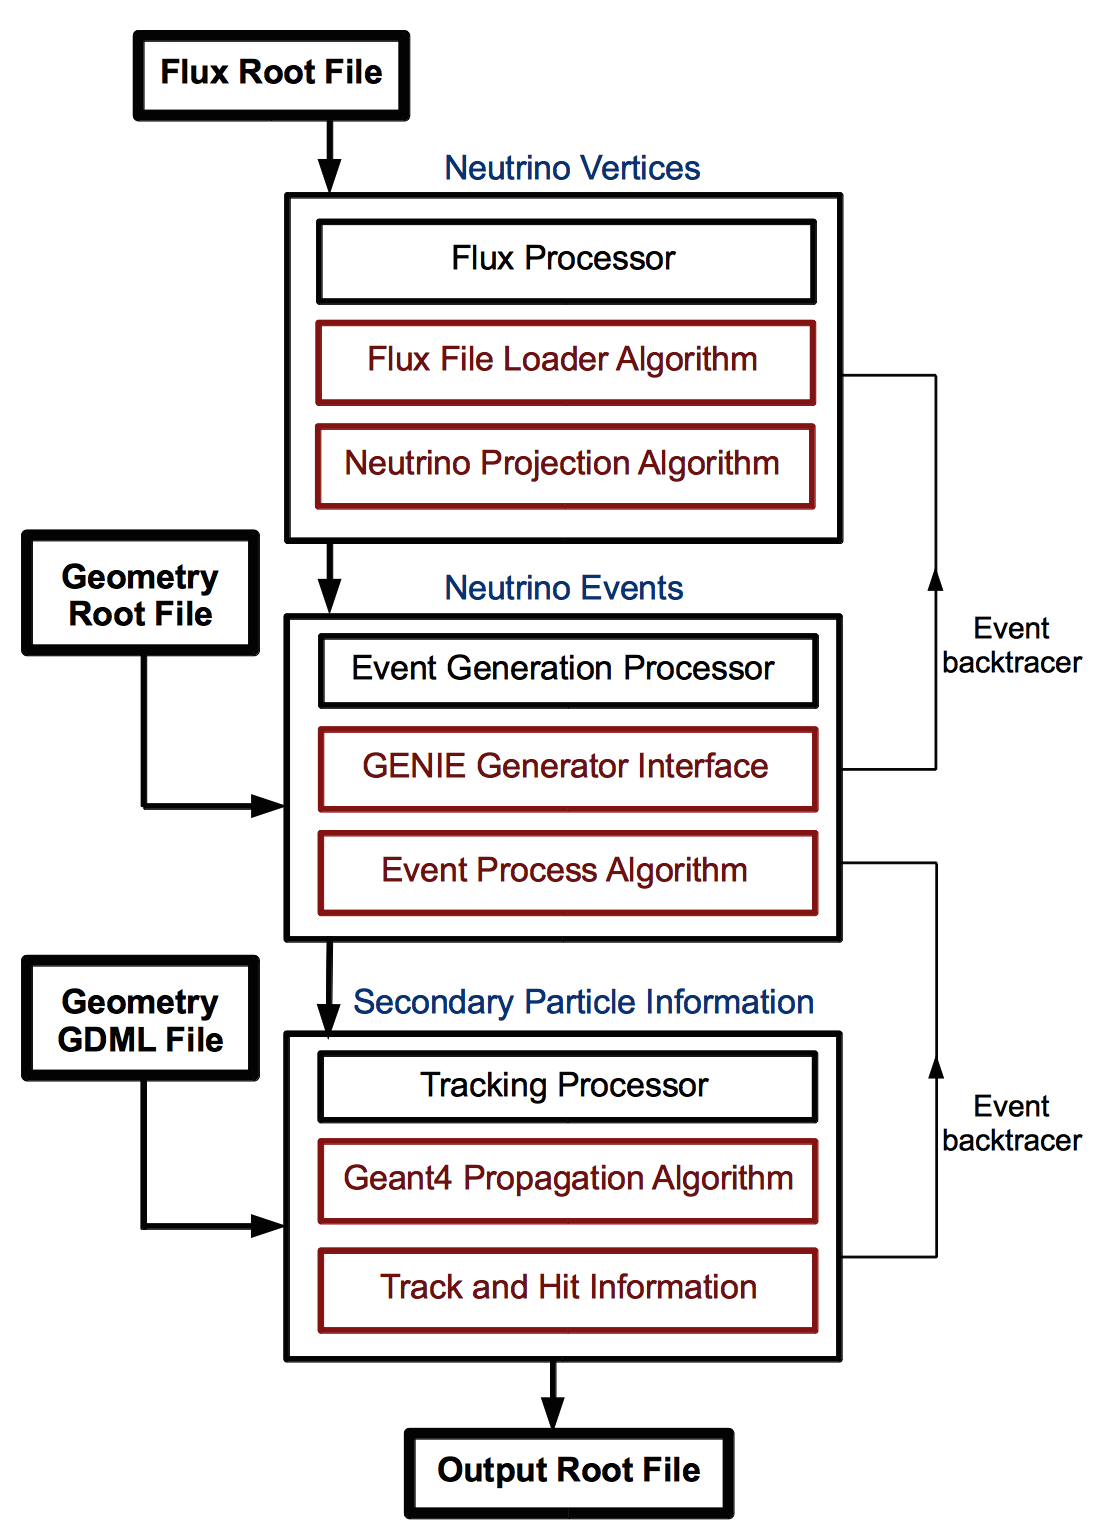
\includegraphics[width=120mm]{Chapter4/figures/softwareProcessDiagram.png}
  \caption{The software architecture used for the MC simulation study for LAGUNA-LBNO.}
  \label{fig:softwareArch}
\end{center}
\end{figure}

\section{Modelling the Near Detector Environment}
Modelling the geometry and its surrounding environment is done within the ROOT geometry package which also provides visualisation of the detector. For neutrino studies it is crucially important to model the materials and orientations of the basic ND components. Finer details are omitted in the geometry, such as structural supports and cabling, as they are assumed to have negligible effect on neutrino interactions. Following from the ND design a close representation is implemented in the software and can be seen in figure \ref{fig:ndGeometry}. Upon construction the details of the geometries material composition and dimensions is written to both .root and .gdml file formats.

\begin{figure}[hbtp]
\begin{center}
  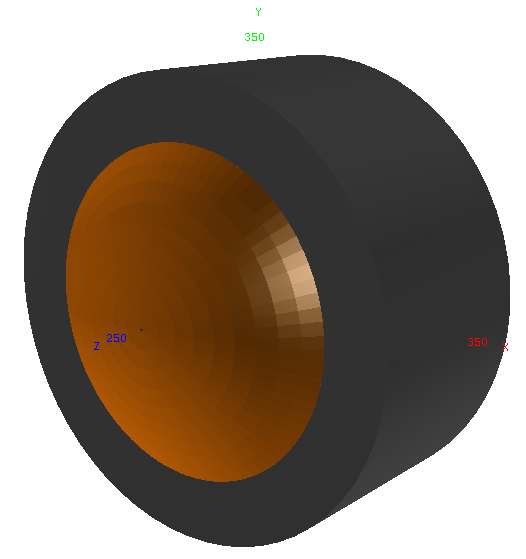
\includegraphics[width=40mm]{Chapter4/figures/nd_closed.png}
  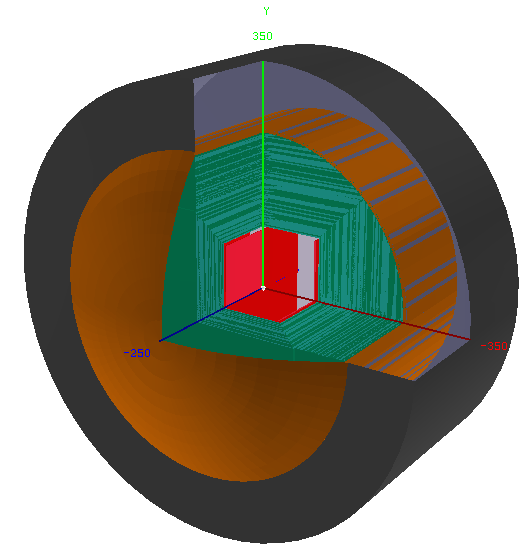
\includegraphics[width=40mm]{Chapter4/figures/nd_partially_open.png} 
  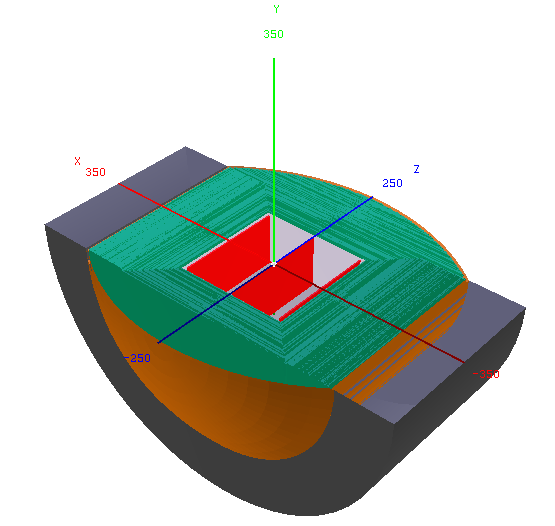
\includegraphics[width=40mm]{Chapter4/figures/nd_open.png}
\end{center}
\begin{center}
  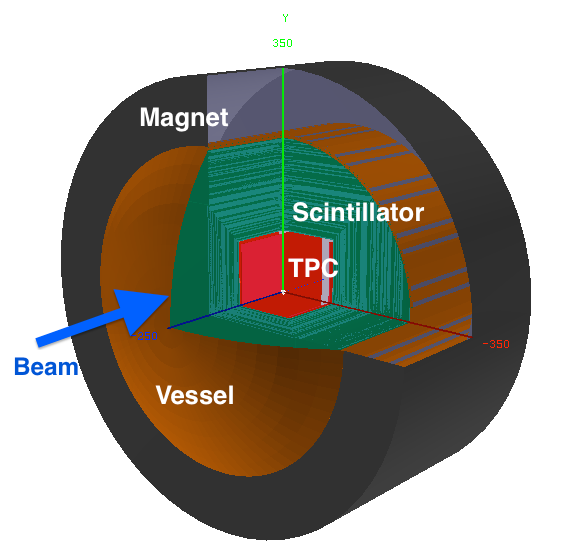
\includegraphics[width=100mm]{Chapter4/figures/nd_labelled.png}
  \caption{Top: Images of the ND geometry in the ROOT display for closed (left), partly open (middle) and cross section (right). Bottom: A fully labelled image showing dimensions in cm with detector chambers labelled.}
  \label{fig:ndGeometry}
\end{center}
\end{figure}

\subsection{TPC}
 The 2 $\times$ 2 $\times$ 2 m$^{3}$ TPC contains GAr at 20 Bar, with a density of 35 kgm$^{-3}$. Quench gases are included at ratios matching that of T2K ND280 \cite{t2kNim}. The pressurised gas is then a mixture consisting of 95\% $^{40}$Ar, 3\% CH$_{4}$ and 2\% Isobutane (C$_{4}$H$_{10}$). The introduction of cathode and anode plates in the TPC reduces this active volume by $\sim$5 kg, with each plate of thickness of 13.2 mm and length and width of 1.9 m with the material composition also based on the ND280 design. The total mass of the gas in the TPC is then 275 kg. 

\subsection{Pressure Vessel}
The vessel is of cylindrical design with the addition of slightly curved ends. This is modelled in the software as a cylinder of 5 m outer diameter as the main section, appended with a spherical cap on each end of total inner radius 4.05 m. This results in a protrusion of 0.825 m for each end. To maintain a 5 m length, the cylinder is of length 3.35 m. A sketch of this implementation with dimensions is shown in figure \ref{fig:vesselSketch}. 50 mm thick aluminium of density 2700 kgm$^{-3}$ is used as the vessel material. The pressure vessel then has a considerable mass of $\sim$8.2 tonnes.

The inner vessel is filled with the same gas composition and pressure as the TPC, with the TPC centred in the middle of the vessel.

\begin{figure}[hbtp]
\begin{center}
  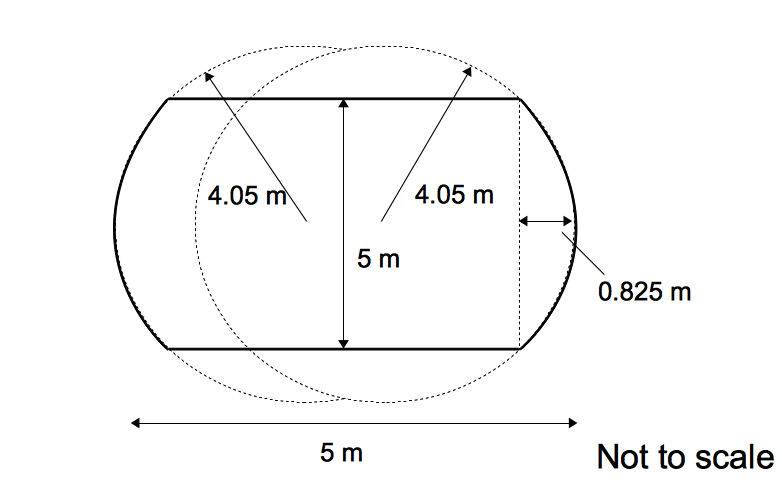
\includegraphics[width=120mm]{Chapter4/figures/vesselDrawing.png}
  \caption{The basic sketch of the side view of the pressure vessel with dimensions in meters. The bold lines indicate the implemented volume. The drawing is not to scale.}
  \label{fig:vesselSketch}
\end{center}
\end{figure}

\subsection{Scintillator}
The scintillator layers are modelled with plastic of composition C$_{5}$O$_{2}$H$_{8}$ and of density 1.18 gcm$^{-3}$. Individual scintillation bars are not implemented in the model, instead layers of 10 mm thickness are used. The first layer consists of six blocks to fully enclose the TPC, covering each face, with additional layers covering each previous layer. Dividing the six faces into pairs of X, Y and Z faces the dimensions of the n$^{th}$ box layer $t \times l_{n} \times h_{n}$ are given by equations \ref{eq:scintXDim} to \ref{eq:scintZDim}. This procedure is followed until the scintillators layers reach the vessel edges or enter the curved ends. In the curved ends the layers are then modelled with circular disc layers of the same thickness but with decreasing radius to match that of the inner vessel radius. However less scintillator layers are added upstream of the TPC to avoid introducing dense material which would increase neutrino interactions upstream of the TPC. Following this implementation strategy the ND scintillator can be summarised by figure \ref{fig:vesselDiagram} with the total dimensions of the detector. The yellow region inside of the pressure vessel then refers to the volume in which scintillator was omitted, remaining as a GAr region at the same pressure as the TPC, as the whole volume inside the vessel is pressurised at 20 bar. The total mass of all the introduced scintillator is then 73.1 tonnes.

\begin{equation}
	X_{n} = 0.01 \times 2(1 + 0.01(n-1)) \times 2(1 + 0.01(n-1)) \hspace{2mm} \textnormal{m}^{3}
	\label{eq:scintXDim}
\end{equation}
\vspace{-6mm}
\begin{equation}
	Y_{n} = 0.01 \times 2(1 + 0.01(n-1)) \times 2(1 + 0.01n) \hspace{2mm} \textnormal{m}^{3}
	\label{eq:scintYDim}
\end{equation}
\vspace{-6mm}
\begin{equation}
	Z_{n} = 0.01 \times 2(1 + 0.01n) \times 2(1 + 0.01n) \hspace{2mm} \textnormal{m}^{3}
	\label{eq:scintZDim}
\end{equation}

\begin{figure}[hbtp]
\begin{center}
  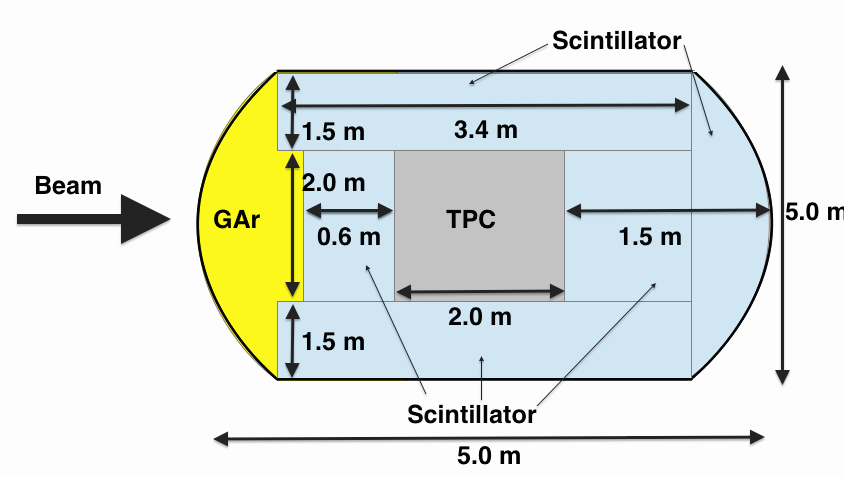
\includegraphics[width=120mm]{Chapter4/figures/vesselDiagram.png}
  \caption{The cross sectional view of the ND vessel with dimensions in meters. The drawing is not to scale.}
  \label{fig:vesselDiagram}
\end{center}
\end{figure}

\subsection{Magnet}
The dipole magnet is modelled as a simple solid cylindrical iron tube. The inner radius is 2.5 m and outer radius of 3.5 m, yielding a thickness of 1 m and has a length of 3.35 m. At a density of 7870 kgm$^{-3}$ the magnet has a mass of 496.7 tonnes. 

The magnetic field is simulated as a dipole of constant magnetic field strength of 0.5 T. The magnetic field is only implemented across the TPC as this is the only area of concern for this study. Taking the beam direction as (0, 0, 1), the electron drift is then perpendicular to this in the (-1, 0, 0) direction and the magnetic field of $\boldsymbol{B}$ = (0.5, 0, 0) T is then anti-parallel to the electric field.

\subsection{The Surrounding Environment}
It is also necessary to model the surrounding environment of the ND to perform background studies on the ND. Specifically this relates to neutrino interactions in the surroundings producing muons which can then reach the ND TPC. A simple model is used composing of a rock environment with an air cavity.

\subsubsection{Cavity}
The cavity replicates the excavation hole needed to insert the ND underground. This is a cylindrical hole of 9 m in diameter and the ND is situated at the bottom of the 23.5 m long hole, giving a volume of 1494.2 m$^{3}$. A simple composition of air (78\% N and 22 \% O) and of density 1.29 kgm$^{-3}$ is used as the medium for the cavity.

\subsubsection{Rock}
Previous excavations at CERN and geological studies have shown that the rock beneath the surface at the proposed ND location consists of mainly sandstone \cite{sandstone}. Sandstone is modelled as a composition of 53\% Oxygen and 47\% Silicon and of constant density 2323 kgm$^{-3}$. This is a simplification but small fluctuations in densities and chemical composition would have negligible effect on background neutrino interactions. With high energy muons capable of passing through large quantities of dense material, $\sim$30 m for 10 GeV muons, the surrounding environment must be extremely large. A 40 $\times$ 40 $\times$ 200 m$^{3}$ = 320,000 m$^{3}$ cuboid volume is implemented to give a modest estimate of the actual environment. Removing the cavity volume, which is centred in the middle of the rock and extends to the top of the rock, then gives a total rock mass of 7.4 $\times$ 10$^{8}$ kg.

The materials implemented in the geometry are summarised in table \ref{tab:ndMatPara} with the overall masses and volumes of each ND component shown in table \ref{tab:ndMatPara2}.

\begin{table}[h]
\centering
\begin{tabular}{lccc}
	\hline
	\textbf{Detector Component} & \textbf{Mass Composition} (\%) & \textbf{Density} \\
	& & [kgm$^{-3}$]  	\\
	\hline
	TPC Gas Mixture - 20 Bar	& Ar(95), C(2.1), H(0.3), F(2.6) & 35  \\
	TPC Cathode/Anode & C(36), O(26), Si(15), H(6), Cu(17) & 287  \\
	Scintillator	 & C(60), O(32), H(8) & 1180  	\\
	Vessel &	Al (100) &	2700	 \\
	Magnet &	Fe (100)  & 7870 \\
	Cavity &N (78), O (22) & 1.29 \\
	Rock & O (53), Si (47) & 2323 \\
	\hline
\end{tabular}
\caption{The material compositions based on mass and densities of each of the materials implemented in the ND geometry in the software model.}
\label{tab:ndMatPara}
\end{table}

\begin{table}[h]
\centering
\begin{tabular}{lccc}
	\hline
	\textbf{Detector Component} & \textbf{Total Volume} & \textbf{Total Mass} \\
	& [m$^{3}$] & [tonnes]  \\
	\hline
	TPC Gas Volume & 7.86 & 0.275\\
	TPC Cathode/Anode & 0.143 & 0.040\\
	Scintillator	 & 62.0 & 73.1 \\
	Vessel & 3.02 & 8.17 \\
	Magnet & 63.1 & 497\\
	Cavity & 1.49 $\times$ 10$^{3}$ & 1.93 \\
	Rock & 320 $\times$ 10$^{3}$ & 7.40 $\times$ 10$^{5}$ \\
	\hline
\end{tabular}
\caption{The total volumes and masses of each of the ND components and surrounding environment used in the software model.}
\label{tab:ndMatPara2}
\end{table}

\section{Event Displays and Visualisation}
Example event displays of neutrino interactions in the ND geometry as seen within the software are shown in figure \ref{fig:eventDisplays}. Three interactions are shown, all within the TPC gas: $\nu_{\mu} + Ar$ $\rightarrow$ $\mu^{-} + n + n + n + p$ (Upper), $\nu_{\mu} + Ar$ $\rightarrow$ $\mu^{-} + p + \pi^{+} + \pi^{-}$ (Middle) and $\nu_{\mu} + Ar$ $\rightarrow$ $\nu_{\mu} + n$ (Lower). The left displays show the X and Z directions which are the magnetic field and beam directions respectively. The right images shows the Y and Z directions. The beam is incident from the left on all event displays. A colour scheme is used to illustrate the different particle types and is described in the figure caption, however all red circles indicate a detector hit, regardless of the particle type which deposited energy in the TPC or TAS.

\begin{figure}[htbp]
\begin{center}
  	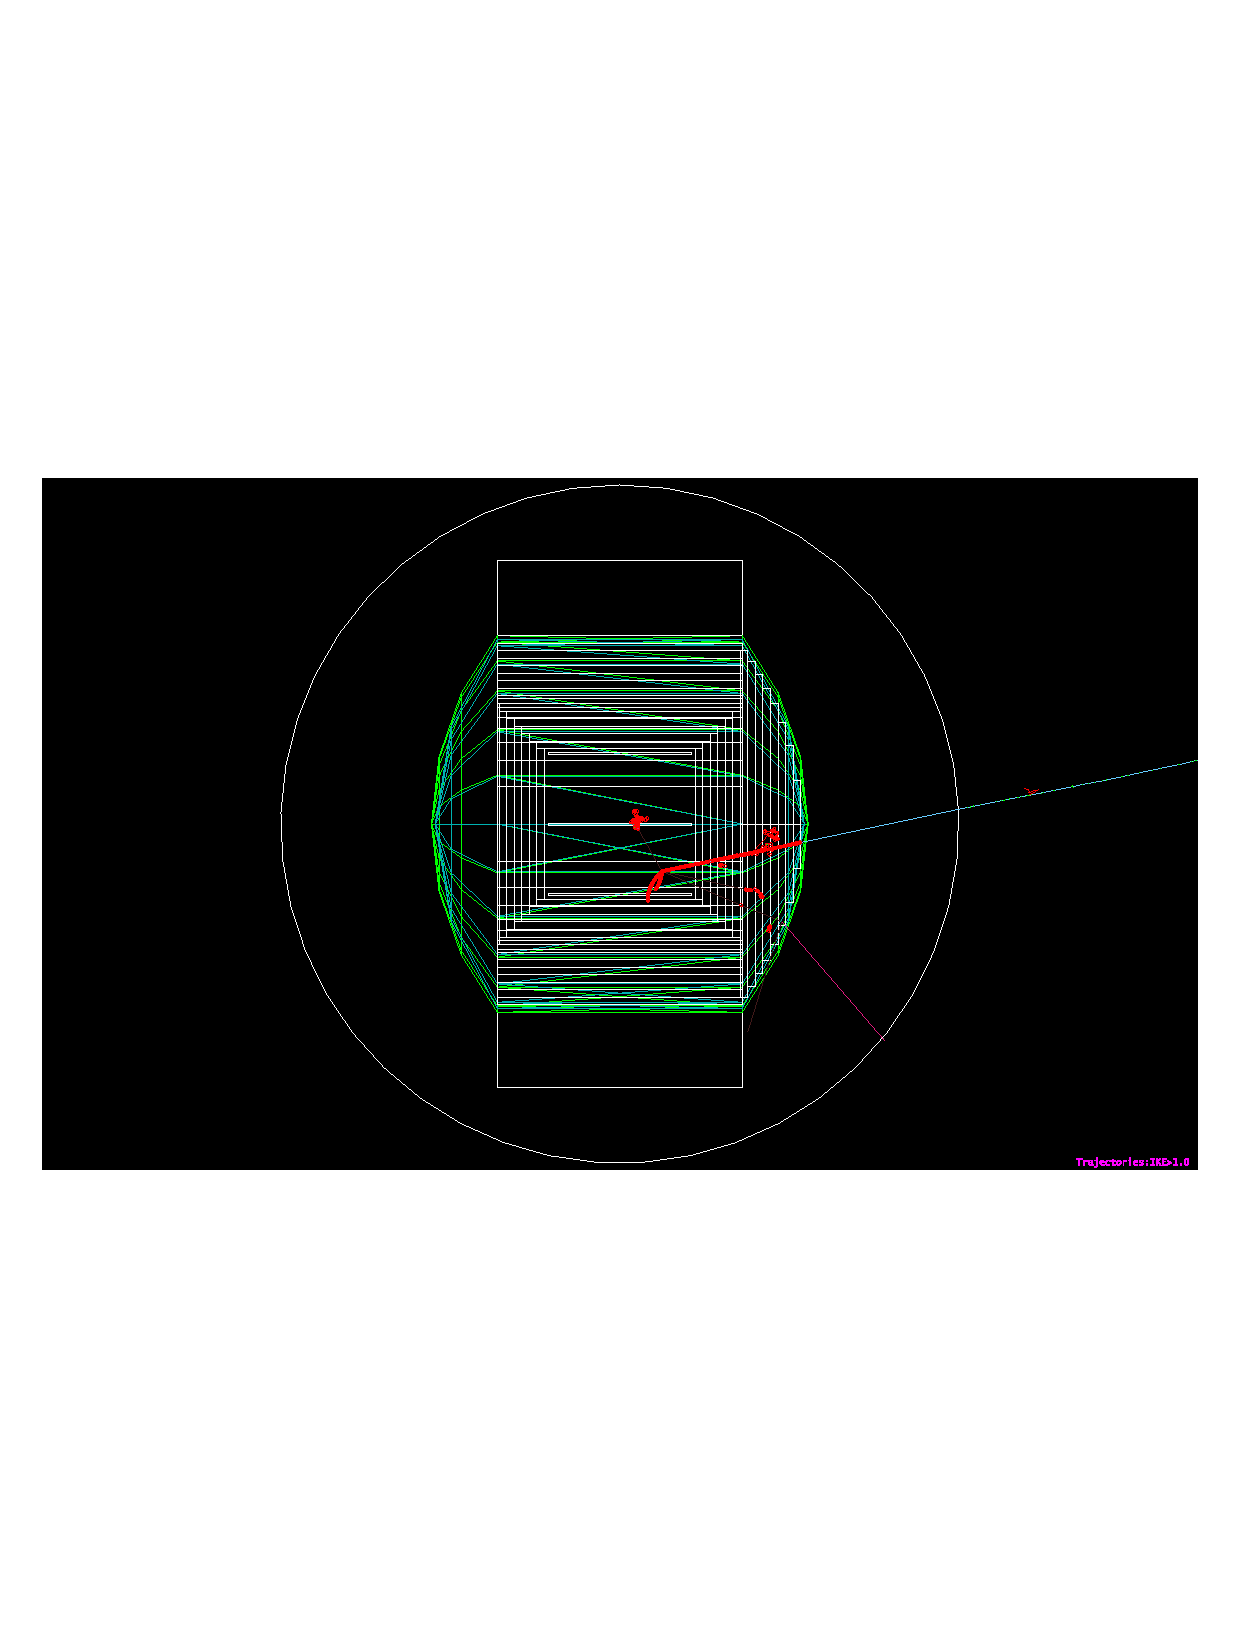
\includegraphics[width=75mm]{Chapter4/figures/eventDisplay_event9_viewXZ.pdf} 
  	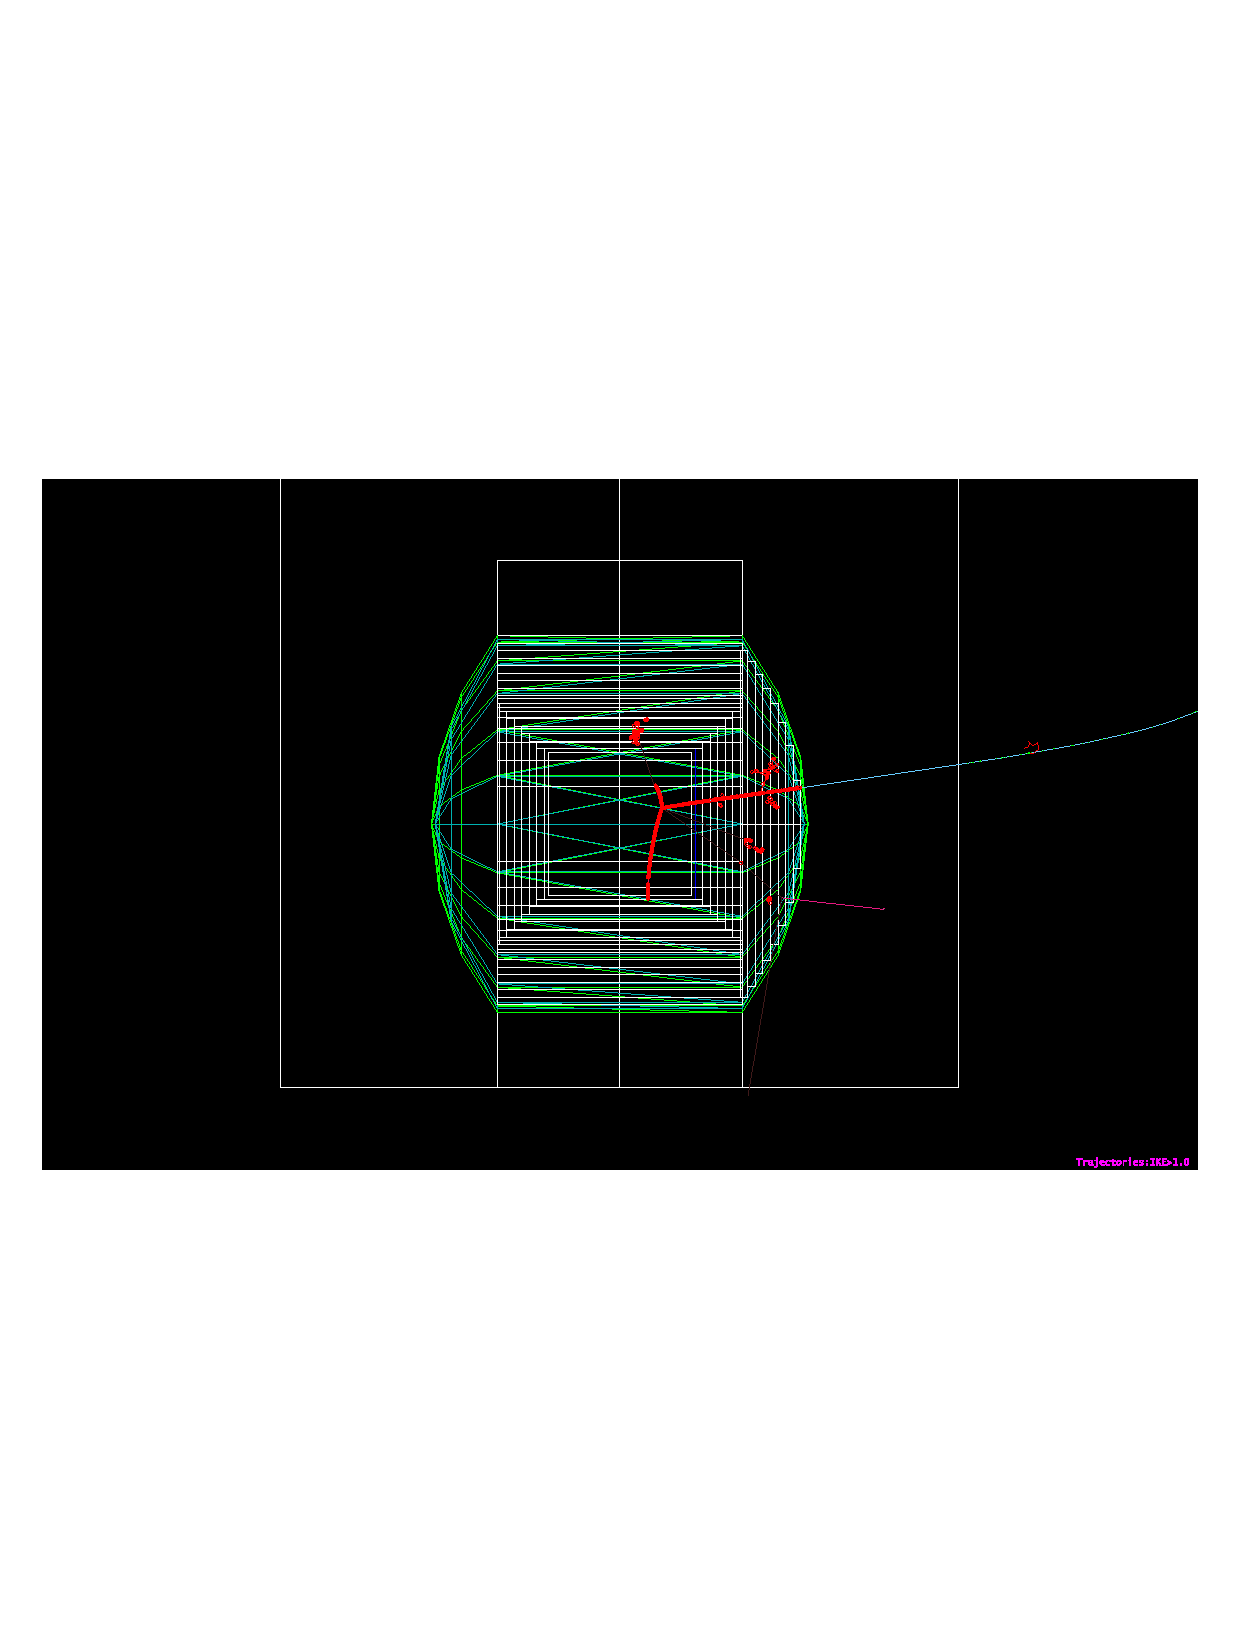
\includegraphics[width=75mm]{Chapter4/figures/eventDisplay_event9_viewYZ.pdf} \\
	\vspace{3mm}
  	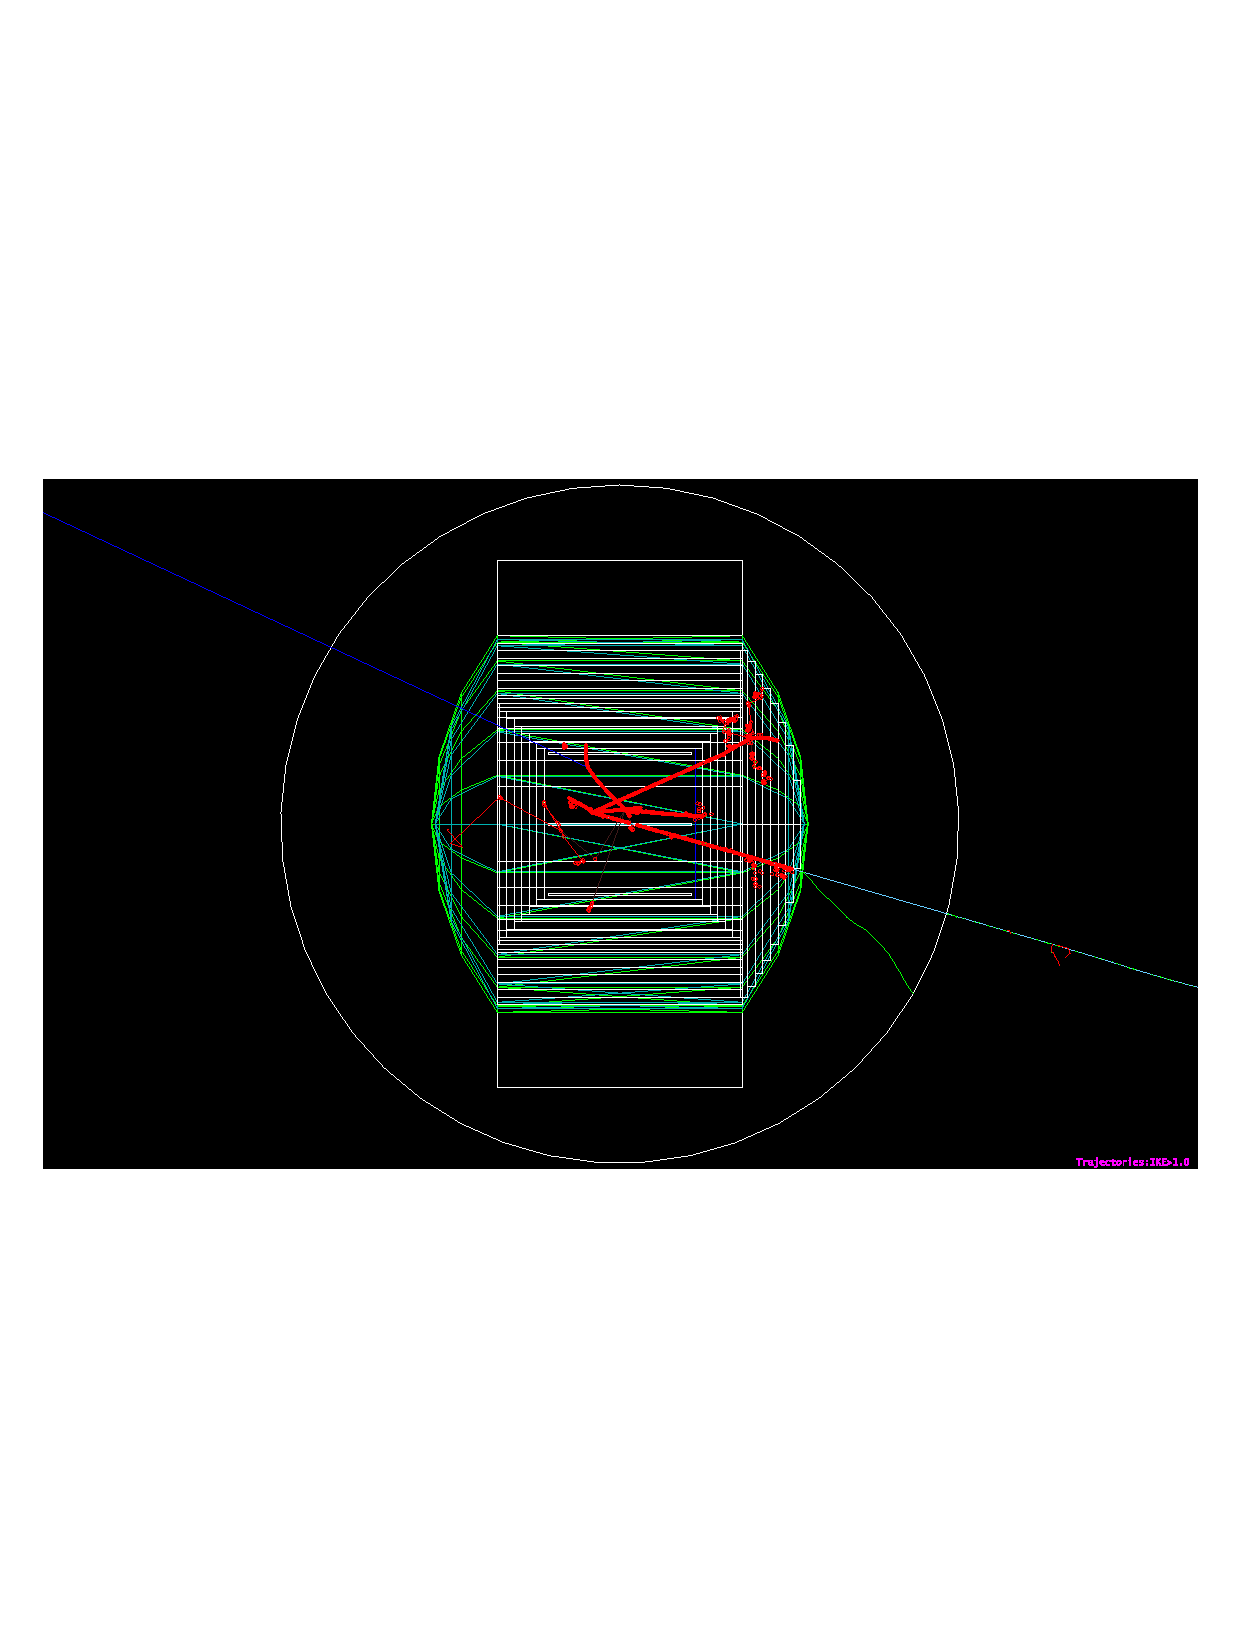
\includegraphics[width=75mm]{Chapter4/figures/eventDisplay_event10_viewXZ.pdf} 
  	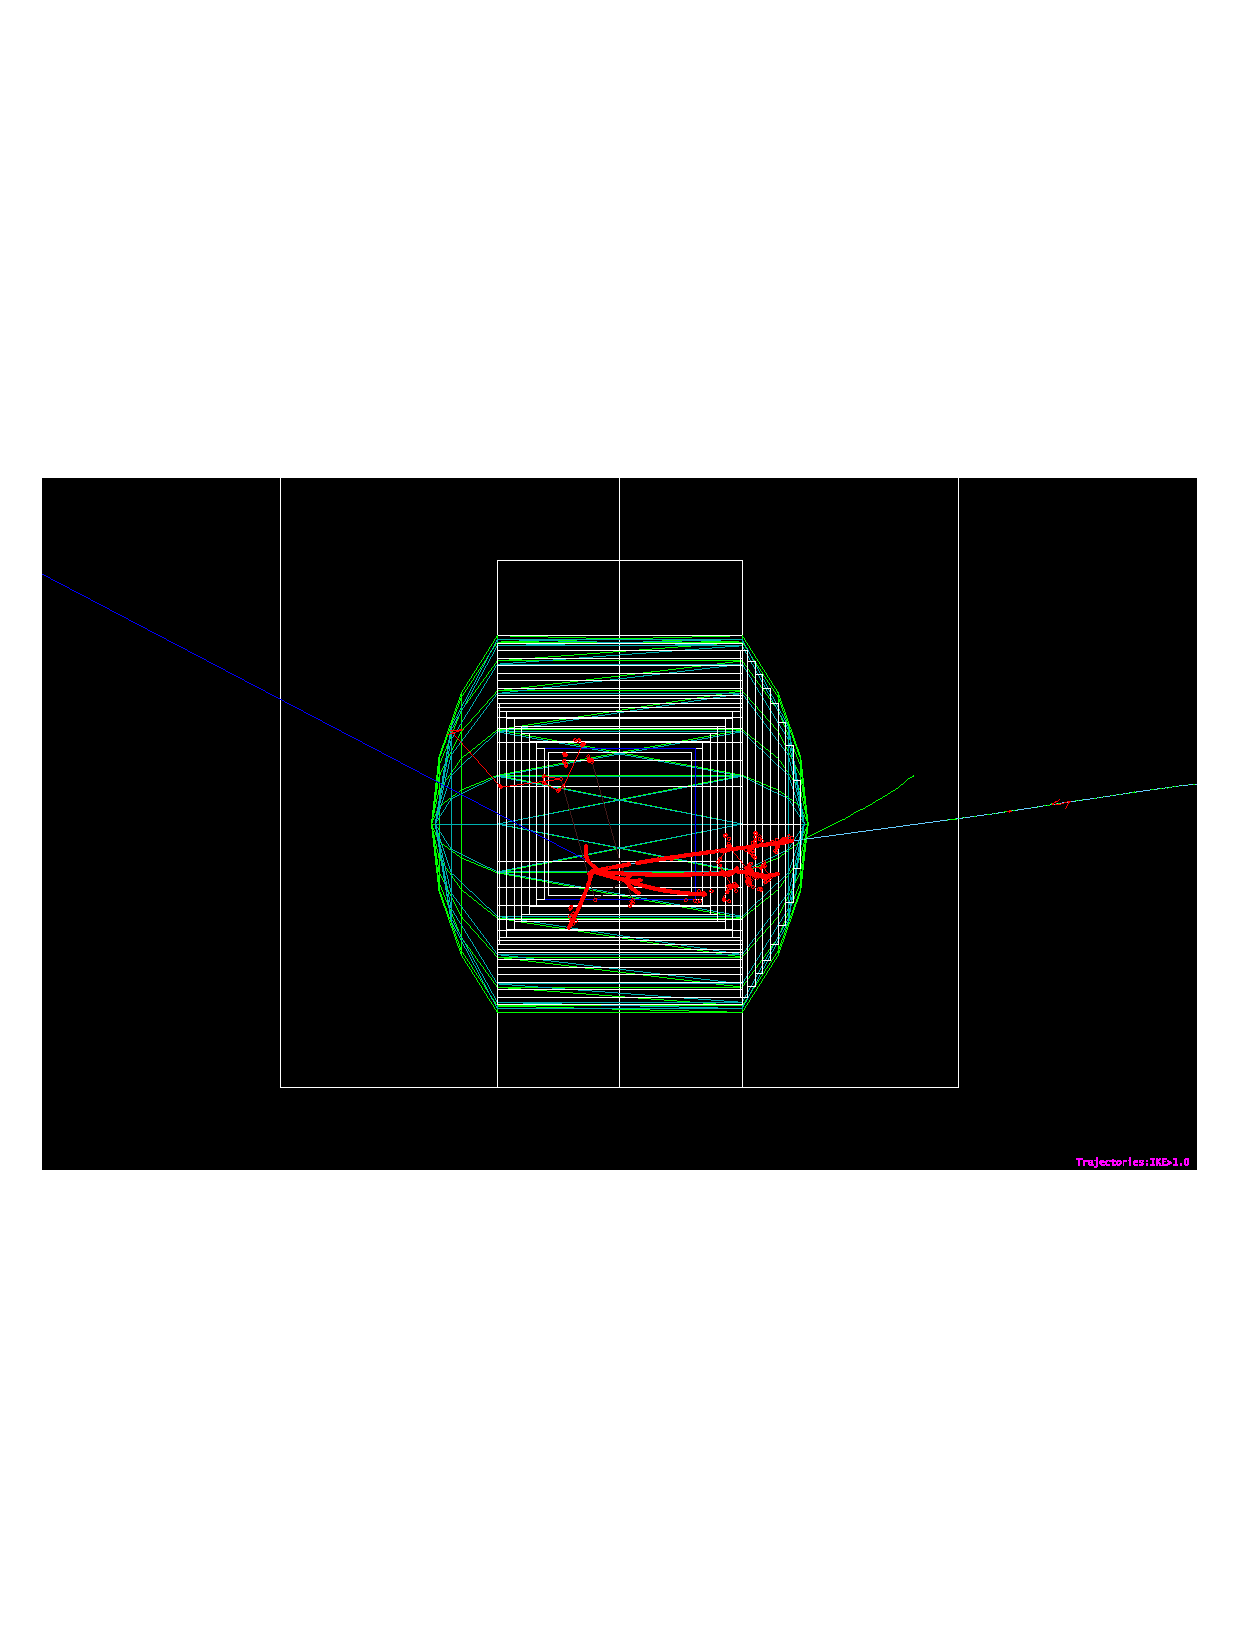
\includegraphics[width=75mm]{Chapter4/figures/eventDisplay_event10_viewYZ.pdf}\\
	\vspace{3mm}
  	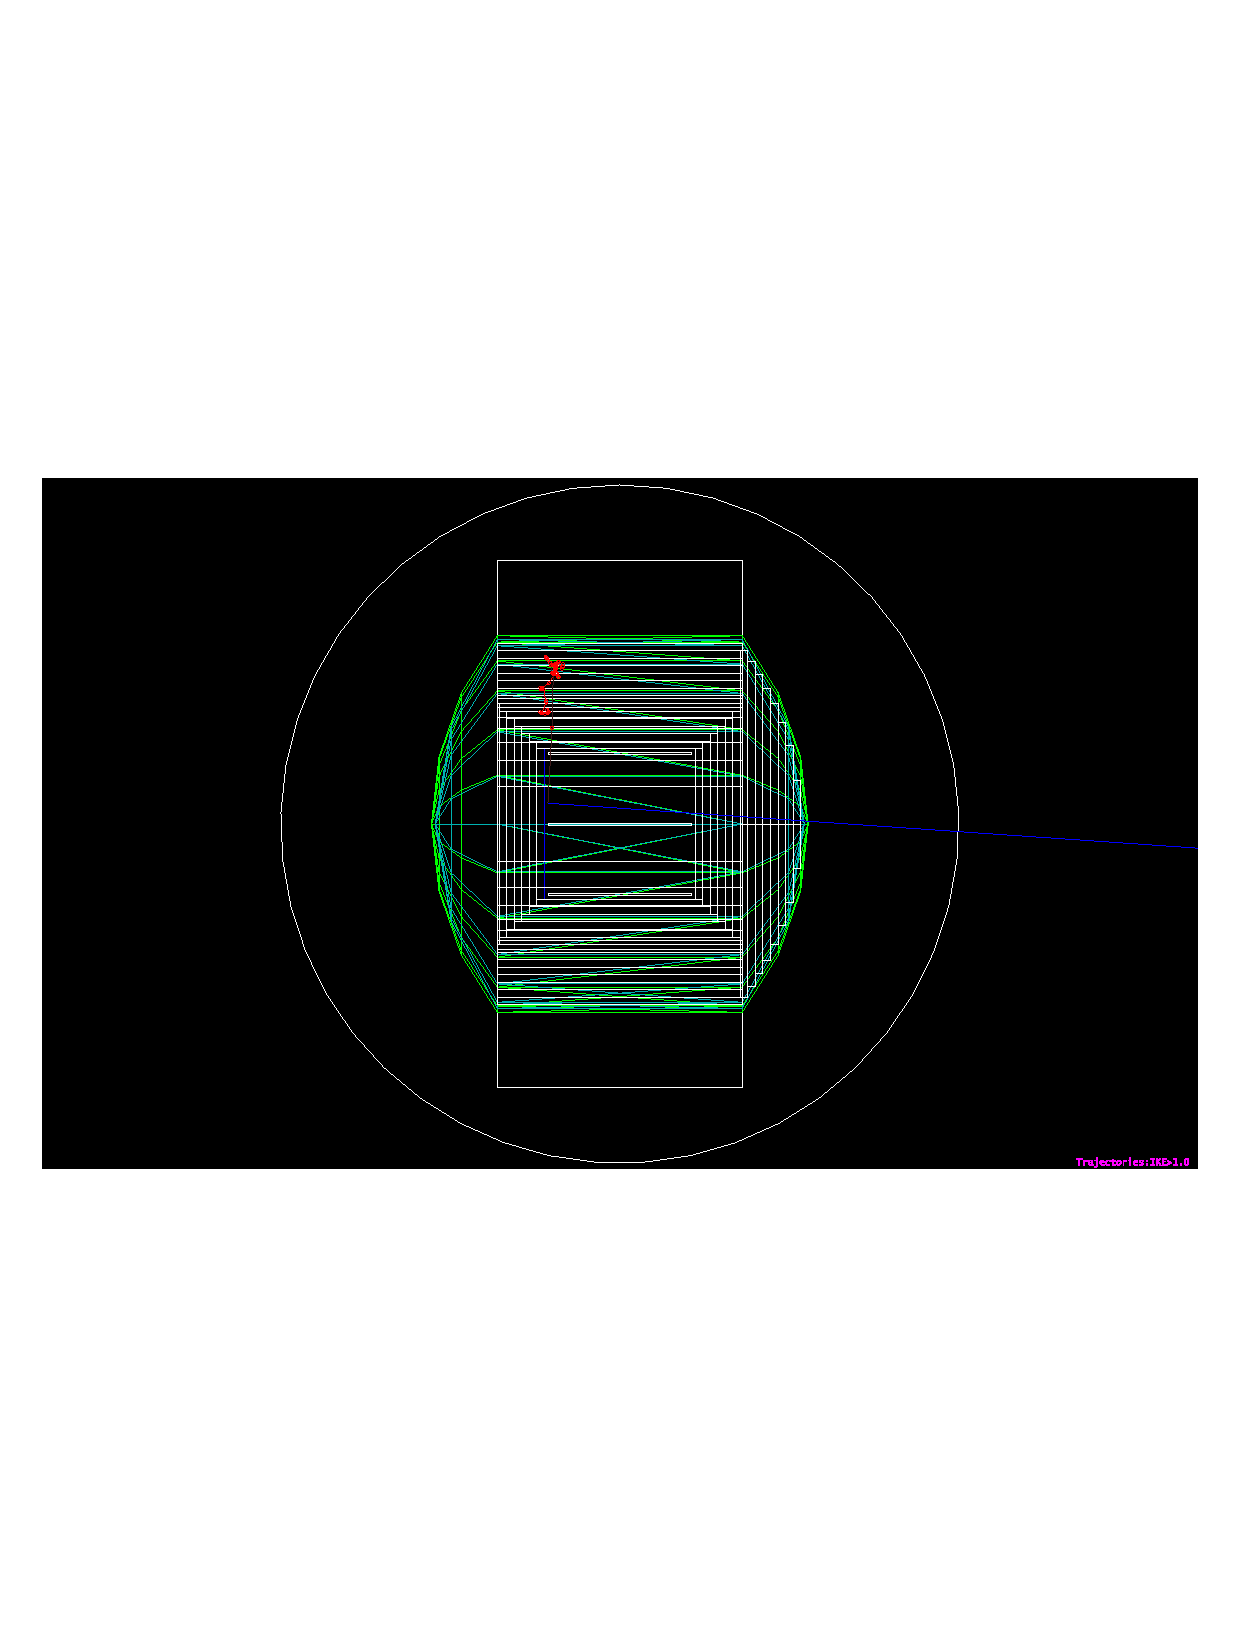
\includegraphics[width=75mm]{Chapter4/figures/eventDisplay_event5_viewXZ.pdf} 
  	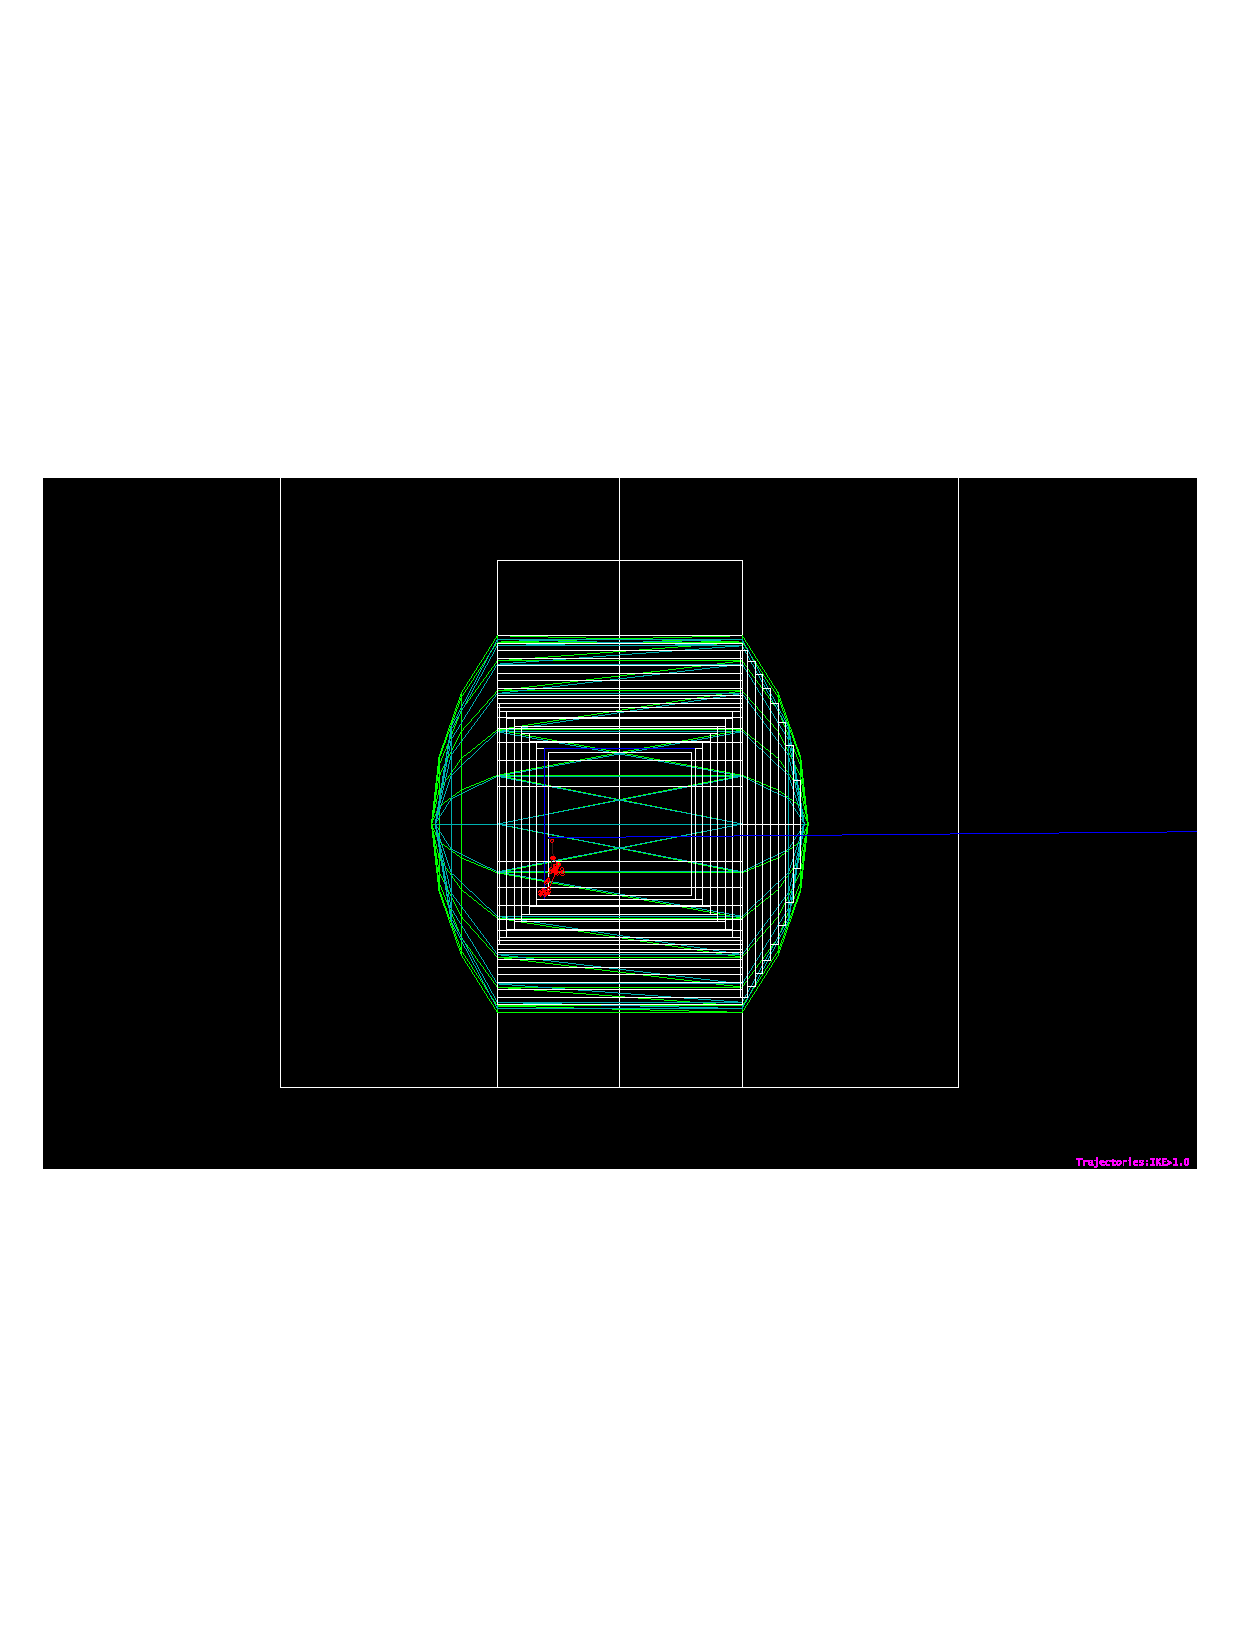
\includegraphics[width=75mm]{Chapter4/figures/eventDisplay_event5_viewYZ.pdf} 
	\caption{Several event displays are shown for interactions: $\nu_{\mu} + Ar$ $\rightarrow$ $\mu^{-} + n + n + n + p$ (Upper), $\nu_{\mu} + Ar$ $\rightarrow$ $\mu^{-} + p + \pi^{+} + \pi^{-}$ (Middle) and $\nu_{\mu} + Ar$ $\rightarrow$ $\nu_{\mu} + n$ (Lower). A colour scheme is used for particle types, neutrons are brown, protons are pink, muons are light blue, electrons are green, neutrinos are dark blue and red circles indicated detector hits from any particle type. The left displays show the X and Z directions which are the magnetic field and beam directions respectively. The right images shows the Y and Z directions. The beam is incident from the left on all event displays.}
	\label{fig:eventDisplays}
\end{center}
\end{figure}

%The detector hits are recorded and their energy deposition is........

\section{The TPC Rates}
When designing a detector it is of primary concern to estimate and understand the number of particle interactions (event rates) occurring. The TPC is the primary target of the detector and it is therefore important to understand all potential particles that can interact or enter the TPC. There are four main contributions that can be considered to estimate these rates, they are:
\begin{enumerate}
\setlength{\itemsep}{0.8pt}
	\item Particles arising from direct neutrino interactions in the TPC
	\item Particles arising from neutrino interactions from the rock and detector surroundings
	\item Particles arising from neutrino interactions from outer detector components
	\item Muons originating from the beam that penetrate through to the TPC
\end{enumerate}
These four areas are summarised in figure \ref{fig:particleBackgrounds}. Except for neutrino interactions directly in the TPC the remainder are all background events. While it will be impossible to eliminate these backgrounds entirely, it may be possible to reduce them with an aim to improve the performance of the TPC.

\begin{figure}[hbtp]
\begin{center}
  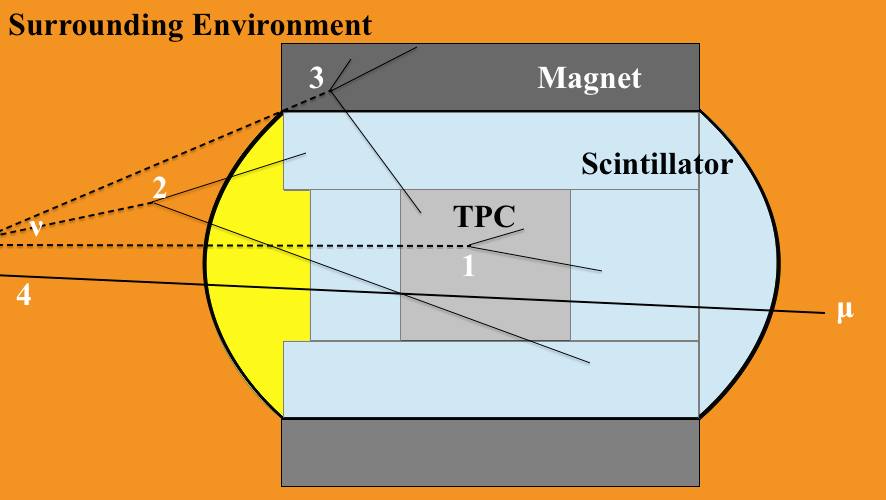
\includegraphics[width=120mm]{Chapter4/figures/particleInteractions.png}
  \caption{A graphic showing the different contributing factors of particles reaching the TPC. 1. Particles arising from direct neutrino interactions in the TPC. 2. Particles arising from neutrino interactions from the rock and detector surroundings. 3. Particles arising from neutrino interactions from outer detector components. 4. Muons originating from the beam that penetrate through to the TPC.}
  \label{fig:particleBackgrounds}
\end{center}
\end{figure}

\section{Neutrino Event Rates in the TPC}
Given the two beam options and two polarities ($\nu_{\mu}$ and $\bar{\nu}_{\mu}$ runs), four different estimations were performed by generating MC events. Only interactions in the TPC were considered and the Secondary Tracking Processor could be omitted for this study, as only the number of neutrino interactions is needed. Although not propagated, the Final State Secondaries (FSS) initial properties were recorded. 

The neutrino interaction rates for each of the beam options is shown in the upper of table \ref{tab:neutrinoTPCRates}, along with the neutrino flavour breakdown. These event rates correspond to 10$^{20}$ p.o.t to provide a normalised comparison between the beam options. 

It is clear from these numbers that the 400 GeV beam option is superior in terms of events per p.o.t which is expected due to higher energy protons. However the 50 GeV option provides a cleaner beam, with a greater percentage of the beam composition consisting of its primary neutrino flavour. It is more important to realise these numbers in terms of ppp, which can then declare whether the TPC can cope with these rates. The 400 GeV option can provide 7 $\times$ 10$^{13}$ ppp while the 50 GeV option can provide 2.5 $\times$ 10$^{14}$ ppp. The former option yields 0.1785 $\pm$ 0.0003 $\nu$ ppp and the latter is a factor $\sim$2.5 smaller at 0.0707 $\pm$ 0.0005 $\nu$ ppp, for positive focusing. Negative focusing yields neutrino interaction rates of 0.0880 $\pm$ 0.0006 $\nu$ ppp and 0.0360 $\pm$ 0.0005 $\nu$ ppp for 400 and 50 GeV options respectively.

The 400 GeV beam with positive focusing provides the highest neutrino rate. With one pulse extracted every 6 seconds (2 spills separated by 50 ms, each of 10.5 $\mu$s) and drift times in Argon of the order of 100 $\mu$s over 1 m means pile up is not an issue in the gas TPC for these rates.

\begin{sidewaystable}
\centering
\begin{tabular}{| l ||cc|cc||cc|cc|}
	\hline
	 & \multicolumn{4}{|c||}{Positive Focusing} &  \multicolumn{4}{c|}{Negative Focusing} \\	 
	 \cline{2-9}
	  & \multicolumn{2}{|c|}{400 GeV} & \multicolumn{2}{c||}{50 GeV} & \multicolumn{2}{c|}{400 GeV} & \multicolumn{2}{c|}{50 GeV}  \\	 
	 \cline{2-9}
	 \textbf{Neutrino} & \multicolumn{8}{|c|}{\textbf{Incident Neutrino Counts / 10$^{20}$ p.o.t (\% of Total)}} \\	 
	 \cline{2-9}
	$\nu_{\mu}$ & 239500 $\pm$ 400 & (93.9\%)& 27700 $\pm$ 200 & (98\%)& 38500 $\pm$ 400 & (30.6\%)& 2070 $\pm$ 70 &(14.2\%)\\
	$\bar{\nu}_{\mu}$ & 14800 $\pm$ 100 & (5.8\%) & 320 $\pm$ 22 & (1\%)& 84600 $\pm$ 600 & (67.2\%)& 12300 $\pm$ 200 & (84.8\%)\\
	$\nu_{e}$ & 665 $\pm$ 23 & (0.3\%) & 299 $\pm$ 21 & (1\%) & 1760 $\pm$ 100 & (1.5\%) & 20 $\pm$ 6 & (0.2\%)\\
	$\bar{\nu}_{e}$ & 0  &(0\%)& 6 $\pm$ 3 & ($<$0.1\%)& 876 $\pm$ 66 & (0.7\%) & 98 $\pm$ 14 & (0.7\%)\\
	\hline
	\textbf{Total} & \multicolumn{2}{|c|}{\textbf{255.0 $\pm$ 0.5 [$\times$10$^{3}$]}} & \multicolumn{2}{|c||}{\textbf{28.3 $\pm$ 0.2 [$\times$10$^{3}$]}}& \multicolumn{2}{|c|}{\textbf{125.7 $\pm$ 0.8 [$\times$10$^{3}$]}} & \multicolumn{2}{|c|}{\textbf{14.4 $\pm$ 0.2 [$\times$10$^{3}$]}}\\
	 \hline
	 \hline	 
	 \cline{2-9}
	 \textbf{Particle} & \multicolumn{8}{|c|}{\textbf{Primaries at Vertex Counts / 10$^{20}$ p.o.t (\% of Total)}} \\
	 \cline{2-9}
	$\mu^{-}$ & 179200 $\pm$ 400 & (10.8\%) & 20700 $\pm$ 200 & (13.5\%) & 28400 $\pm$ 400 & (3.6\%) & 1570 $\pm$ 60& (2.1\%) \\
	$\mu^{+}$ & 10600 $\pm$ 100 &  (0.6\%) & 236 $\pm$ 18 & (0.15\%) & 60500 $\pm$ 500 & (7.7\%) & 8560 $\pm$ 140&  (11.6\%) \\
	$p$ & 475700 $\pm$ 600 & (28.6\%) & 50940 $\pm$ 400 & (33.6\%) &217000 $\pm$ 1000 & (27.5\%) & 22300 $\pm$ 230& (30.3\%) \\
	$n$ & 391700 $\pm$ 600 & (23.5\%) & 38500 $\pm$ 200 & (25.4\%) & 199000 $\pm$ 1000 & (25.2\%) & 20900 $\pm$ 220& (28.5\%) \\
	$\pi^{+}$ & 207800 $\pm$ 400 & (12.5\%) & 14800 $\pm$ 200 & (9.8\%) & 70300 $\pm$ 600 & (8.9\%) & 3680 $\pm$ 90& (5.0\%) \\
	$\pi^{0}$ & 199500 $\pm$ 400 & (12.0\%) & 13100 $\pm$ 200 & (9.0\%) & 91300 $\pm$ 700 & (11.6\%) & 6150 $\pm$ 120& (8.4\%)  \\
	$\pi^{-}$ & 112100 $\pm$ 300 & (6.7\%) & 5850 $\pm$ 90 & (4.0\%) & 79500 $\pm$ 600 & (10.1\%) & 6710 $\pm$ 120& (9.1\%) \\
	$\gamma$ & 19000 $\pm$ 100 & (1.2\%) & 527 $\pm$ 29 & (0.3\%) & 7670 $\pm$ 190 & (1.0\%) & 278 $\pm$ 25& (0.4\%)  \\
	$e^{-}$ & 621 $\pm$ 23 & (<0.1\%) & 241 $\pm$ 20 & (0.2\%) & 1340 $\pm$ 80 & (0.2\%) & 5 $\pm$ 3& (<0.1\%) \\
	$e^{+}$ & 114 $\pm$ 10 & (<0.1\%) & 14 $\pm$ 5 & (<0.1\%) &653 $\pm$ 57 & (0.1\%) & 62 $\pm$ 12& (0.1\%) \\
	other & 66700 $\pm$ 200 & (4.0\%) & 6210 $\pm$ 90 & (4.0\%) & 33000 $\pm$ 400 & (4.1\%) & 3310 $\pm$ 90 & (4.5\%) \\
	\hline
	\textbf{Total} & \multicolumn{2}{|c|}{\textbf{1663 $\pm$ 1 [$\times$10$^{3}$]}} & \multicolumn{2}{|c||}{\textbf{151.6 $\pm$ 0.6 [$\times$10$^{3}$]}} & \multicolumn{2}{|c|}{\textbf{788 $\pm$ 2 [$\times$10$^{3}$]}} & \multicolumn{2}{|c|}{\textbf{73.6 $\pm$ 0.4 [$\times$10$^{3}$]}}\\
	\hline
	Multiplicity & \multicolumn{2}{|c|}{6.52 $\pm$ 0.01} & \multicolumn{2}{|c||}{5.36 $\pm$ 0.04} & \multicolumn{2}{|c|}{6.30 $\pm$ 0.03} & \multicolumn{2}{|c|}{5.08 $\pm$ 0.07} \\
	\hline
	\hline
\end{tabular}
\caption{These rates correspond to neutrino interactions in the TPC GAr volume, based on simulations of various exposures and scaled to a common exposure of 1 $\times$ 10$^{20}$ p.o.t. No fiducial cuts are employed. Statistical errors of $\pm \sigma = \sqrt{n}$ are shown. }
\label{tab:neutrinoTPCRates}
\end{sidewaystable}

Certain selections can be made on the events which are then useful for reconstruction purposes. The event rates already discussed include a selection on the TPC itself, requiring that the events are within the gas and not the cathode/anode plates placed within the TPC. Omitting this selection yields an original neutrino rate of 0.2189 $\pm$ 0.0004 ppp for the 400 GeV PF beam. Taking this event rate as the basis, a series of selections are performed on this and shown in table \ref{tab:nuEventSelection}. Selecting only events within the gas result in a 18.1\% loss in rate. 

Fiducial cuts are necessary for reconstruction purposes as events near the TPC boundaries will be difficult to reconstruct the event with some charged particles leaving the TPC without sufficient track lengths inside the TPC. A 20 cm fiducial cut is applied to each TPC boundary such that event vertices falling within less than 20 cm from a TPC wall are rejected. This dramatically reduces the event rate to 42.2\% which follows in accordance with the volume ratio of 4.05/7.86 = 0.515. 

The energy regime of the neutrino beam is taken from 0 to 30 GeV in the simulations but reconstruction of neutrinos at the high energy end will be more difficult to reconstruct, primarily due to high momentum secondaries having low sagitta values. For oscillation purposes LAGUNA-LBNO is concerned with neutrino energies up to $\sim$10 GeV, a selection of this energy range yields a further reduction of events to 29.7\%. Including only muon neutrinos ($\nu_{\mu}$ only, not $\bar{\nu}_{\mu}$) reduces this by a further 1\%. With CC interactions making up $\sim$75\% of events, we are then left with 21.6\% of neutrino events in the TPC matching all criteria. CCQE interactions account for just 3.6\% of events in the TPC after all the selections but are useful for reconstruction as a measurement of the muon's momentum alone can determine the neutrino energy from equation \ref{eq:ccqeNuEnergy}.

\begin{table}[htbp]
	\begin{center}
	\begin{tabular}{|c||c|c|c|}
		\hline  
		& \textbf{count [1$\times$ 10$^{20}$]} & \textbf{count [ppp]} & \textbf{\% of original} \\
		\hline
		{In TPC} & 313000 $\pm$ 600 & 0.2189 $\pm$ 0.0004 &  {100.0} \\
		{Gas Only} & 255000 $\pm$ 500 & 0.1785 $\pm$ 0.0003 & {81.9} \\
	 	{20 cm Fiducial Cut} & 132000 $\pm$ 400 & 0.0924 $\pm$ 0.0002 & {42.2} \\
		{0 - 10 GeV} & 92800 $\pm$ 300 & 0.0650 $\pm$ 0.0002 & {29.7} \\
		{$\nu_{\mu}$} & 89800 $\pm$ 300 & 0.0628 $\pm$ 0.0002 & {28.7} \\
		{CC} & 67500 $\pm$ 300 & 0.0473 $\pm$ 0.0002 & {21.6} \\
		{CCQE} & 11100 $\pm$ 100 & 0.00779 $\pm$ 0.00007 & {3.6} \\
		\hline
	\end{tabular}
	\end{center}
	\caption{Event rates for neutrino interactions in the TPC after a series of selection criteria are imposed on the events. All events correspond to 400 GeV PF beam option.}
	\label{tab:nuEventSelection}
\end{table}

\subsection{Secondary Particle Production}
The Final State Primary Lepton (FSPL) and Final State Secondaries (FSS) generated at each neutrino vertex are shown in the lower of table \ref{tab:neutrinoTPCRates}. High multiplicites can be expected from the neutrino interactions with average particle multiplicites of 6.52 $\pm$ 0.01 (stat) for the 400 GeV beam option. This is largely due to the high number of DIS events which can be seen from the particle interaction types in table \ref{tab:neutrinoInteractionTypes}. Concerning the number of muons per neutrino interaction, we can expect a muon to be generated at $\sim$70\% of the time, that is 0.1254 $\pm$ 0.0003 (stat) $\mu$ ppp. The energy spectrum of the muons can be seen in figure \ref{fig:muonEnergySpectrum} and illustrates that the majority of the muons generated in the TPC have energies less than 5 GeV while the mean energy is 4.8 GeV.
\begin{table}[tbp]
\centering
\begin{tabular}{ccc}
	\hline
	& \multicolumn{2}{c}{\% of Total Interactions} \\
	\hline
	 \textbf{Type} & \textbf{CC} & \textbf{NC} \\
	 \hline
	 \hline
	 QEL & 9.7 & 3.1\\
	 RES & 14.2 & 5.7 \\
	 DIS & 50.3 & 16.4\\
	 Coherent & 0.4 & 0.2 \\
	\hline
\end{tabular}
\caption{The different interaction types that the neutrino can undergo in GENIE for both CC and NC interactions. The percentage of each type is shown for the number of total interactions.}
\label{tab:neutrinoInteractionTypes}
\end{table}

\begin{figure}
\begin{center}
  	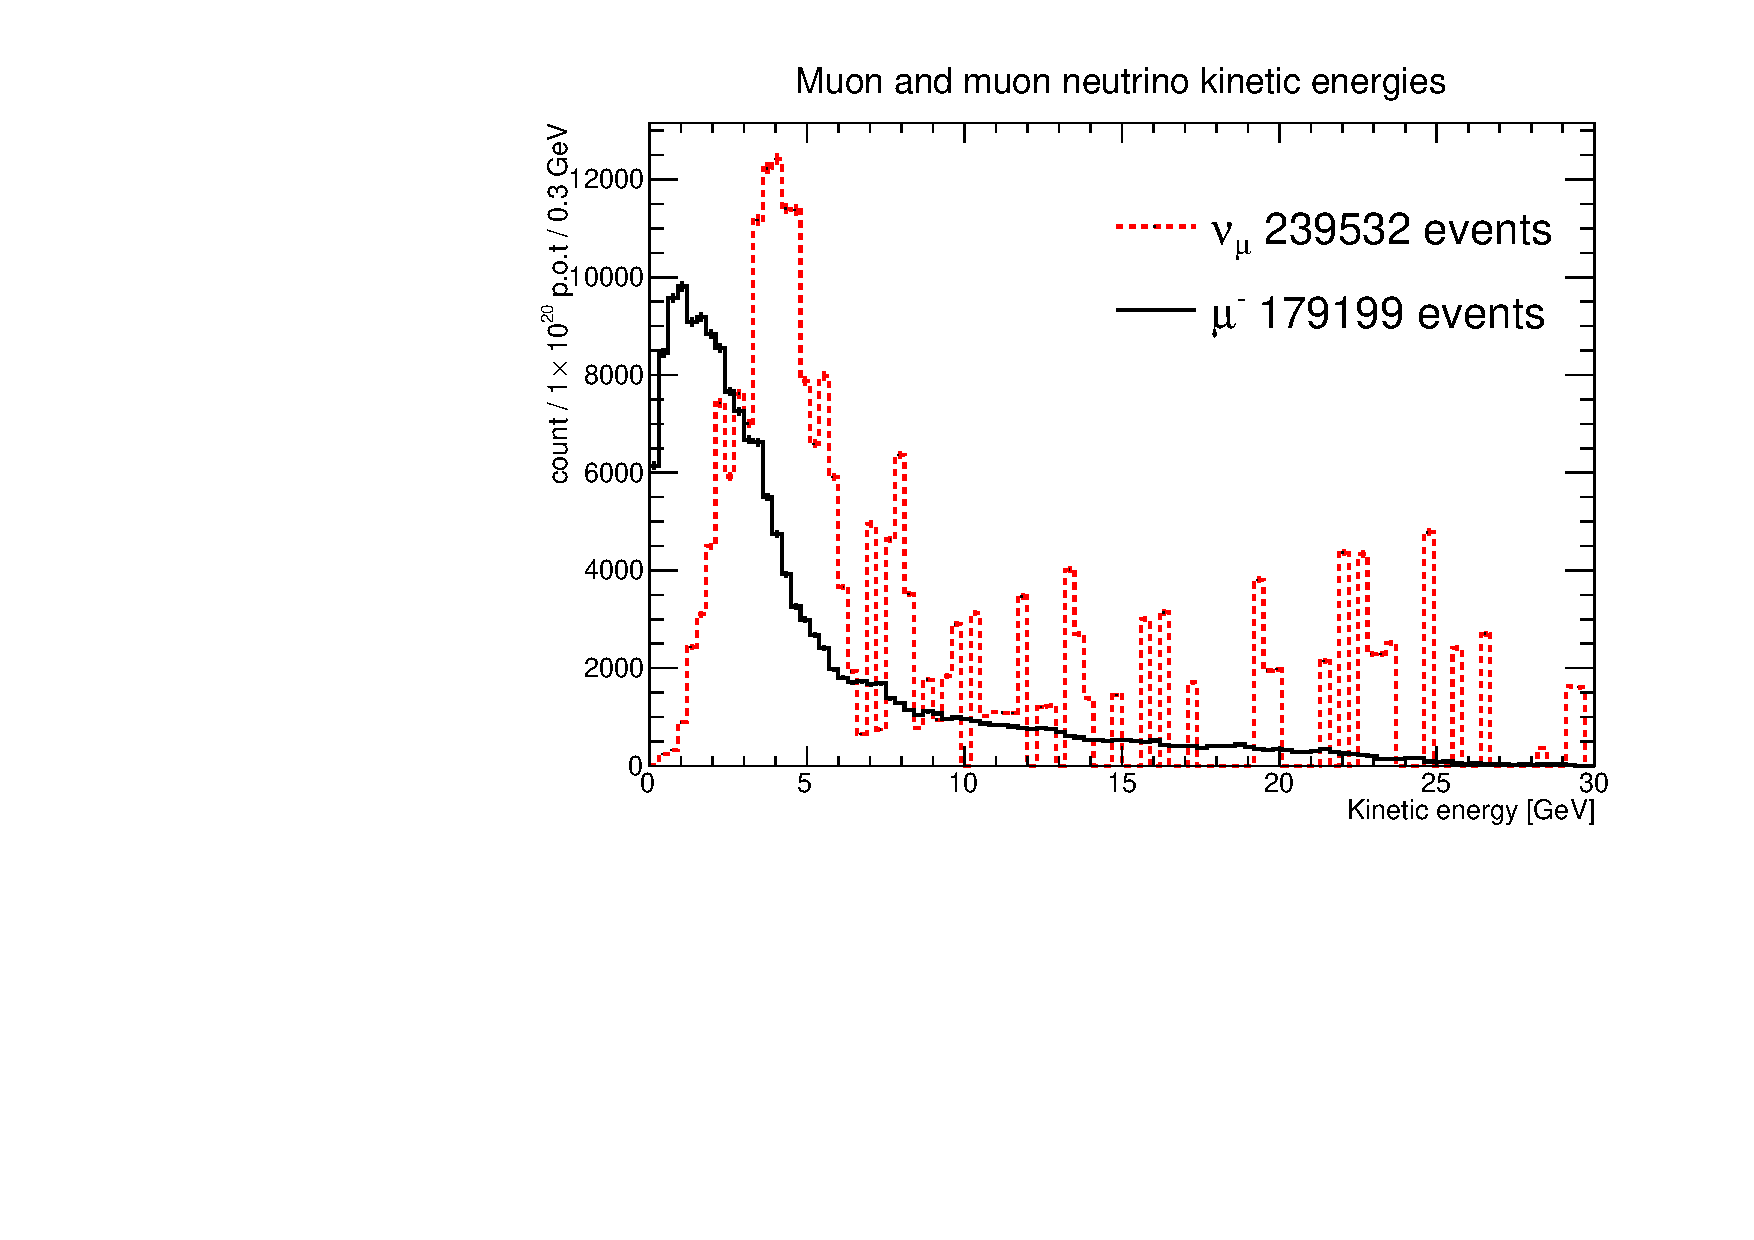
\includegraphics[width=105mm]{Chapter4/figures/muon_and_muNeutrino_kinEnergies.pdf}
	\caption{The kinetic energy spectrum of primary muons (in black) generated at the neutrino vertex in the TPC. The red dashed line indicates the $\nu_{\mu}$ energy spectrum for those causing interactions in the TPC, hence is not simply the flux but is convoluted with the cross section. Counts are normalised to 1 $\times$ 10$^{20}$ p.o.t for 400 GeV PF beam option.}
	\label{fig:muonEnergySpectrum}
\end{center}
\end{figure}

The kinetic energy that each of the secondary particles carries away from the neutrino interaction needs to be understood to establish the ND capabilities for neutrino energy reconstruction. Only charged particles are visible in the TPC whereas other particles of concern such as neutrons and photons are not. By defining the ratio of kinetic energy devoted to charged particles per neutrino event, $T_{c}$, as $\epsilon_{c} = T_{c}/T_{TOT}$ we can understand what is achievable within the TPC. Similarly for neutrons and photons (including those originating from $\pi^{0}$s)  we can define ratios as $\epsilon_{n} = T_{n}/T_{TOT}$ and $\epsilon_{\gamma} = T_{\gamma}/T_{TOT}$ respectively. Figure \ref{fig:CCandNCKinEnergyRatios} shows these ratios for both CC and NC interactions. In NC interactions the outgoing neutrino carries away a significant amount of energy in the majority of interactions and this cannot be detected. Whereas in CC interactions most of the energy is carried by charged particles with little going to photons and neutrons. With $\sim$75\% of neutrino interactions of CC type, the TPC alone will be instrumental in neutrino energy reconstruction.

\begin{figure}
\begin{center}
  	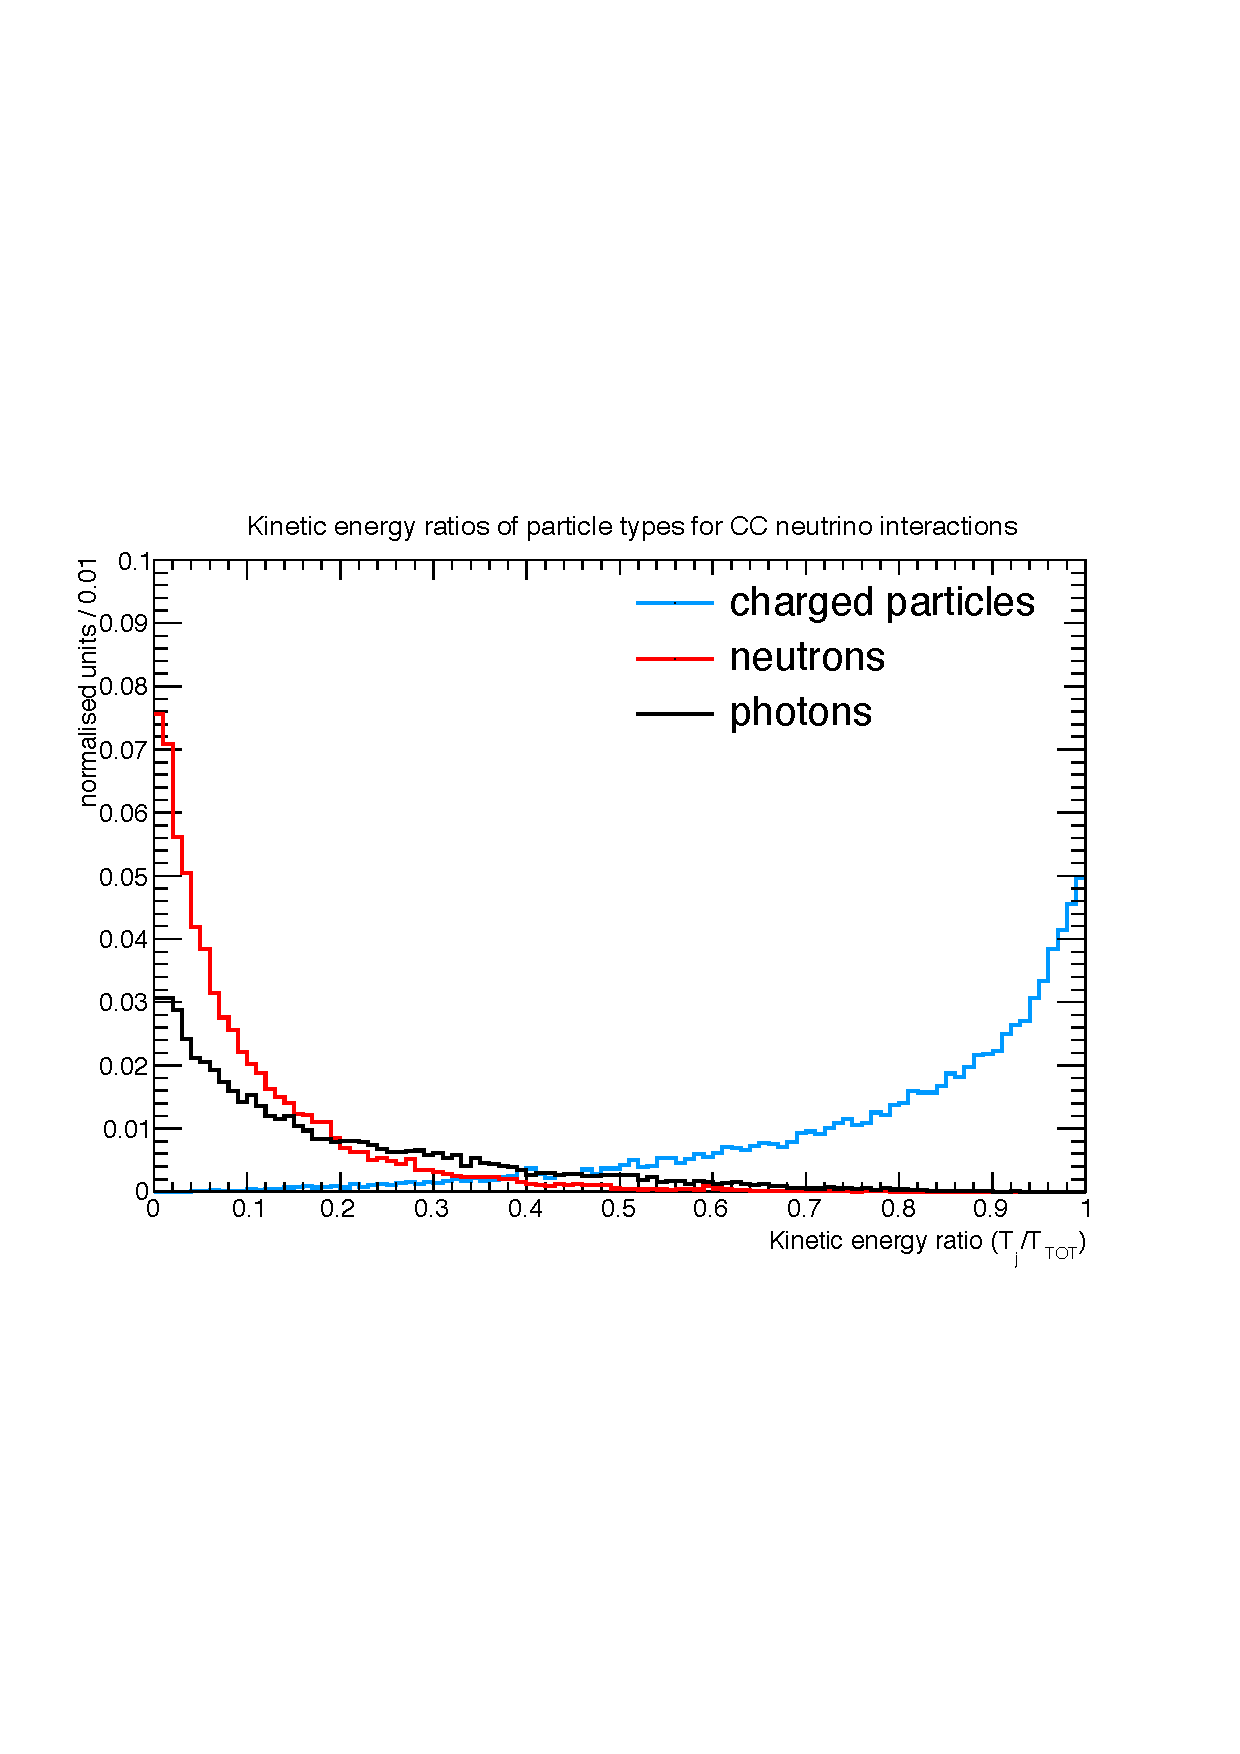
\includegraphics[width=76mm]{Chapter4/figures/cc_kinEnergy_ratio.pdf}
  	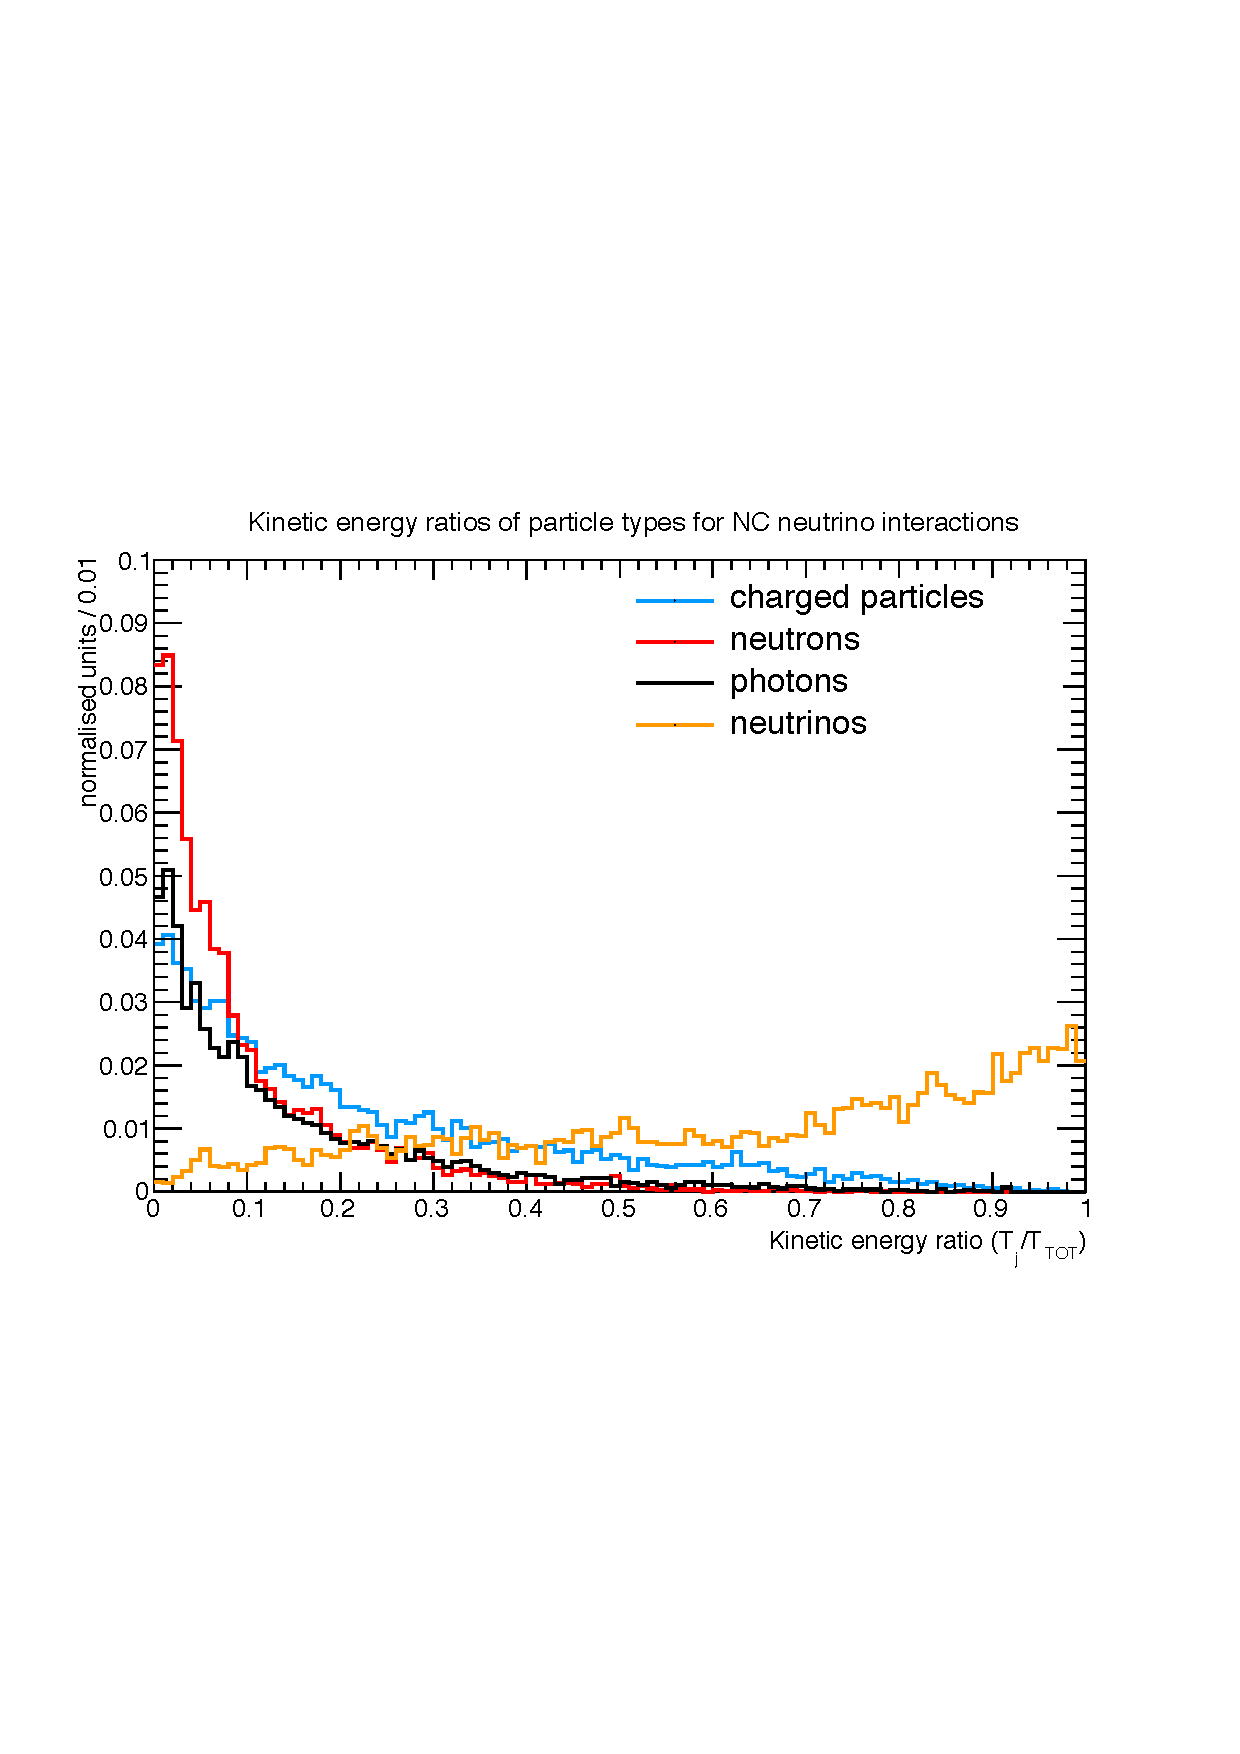
\includegraphics[width=76mm]{Chapter4/figures/nc_kinEnergy_ratio.pdf}
	\caption{The kinetic energy ratios showing the proportion of kinetic energy devoted to charged particles, $\epsilon_{c}$ in blue, neutrons, $\epsilon_{n}$ in red and photons, $\epsilon_{\gamma}$ in black for CC (left) and NC (right) neutrino interactions. The orange line represents the neutrino energy ratio for NC only. Counts are normalised to the number of neutrino events for CC (64238 events) and NC (21292 events) channels. Particles with zero kinetic energy ratios are omitted such that 0 $<$ $\epsilon_{j}$ $\leq$ 1.}
	\label{fig:CCandNCKinEnergyRatios}
\end{center}
\end{figure}

\section{Particles Reaching the TPC}
Particles reaching the TPC from neutrino interactions within the rock surroundings and other detectors components are a background that need to be well understood in order to estimate the TPC performance. These rates can be significant with rock muons (muons originating from neutrino interactions in the rock and the detector environment) produced with high energies (up to 30 GeV). As a result these muons can travel vast distances, up to 60 m, as figure \ref{fig:rockMuonsRange} shows the distances that the muons have travelled to reach the TPC. This is not an indication to their full range as propagation after leaving the TPC is not included in these results. The number of these muons reaching the TPC is considerable at 44.5 $\pm$ 0.5 (stat) ppp for the 400 GeV PF beam option, that is over 350 times that of the muons generated in the TPC. However if only neutrinos with energy of 10 GeV or less are considered this number is more than halved to 19.9$\pm$ 0.2 (stat) ppp, as their range is reduced dramatically. The energy distribution of the muons from the full simulation (up to 30 GeV neutrinos) is shown in figure \ref{fig:rockMuonEnergy}. The energy distributions are very similar when compared to the muons produced inside the TPC but almost all of the muons originating from outside the TPC will enter and leave the TPC and hence have no interaction vertex. 
\begin{figure}[htbp]
\begin{center}
  	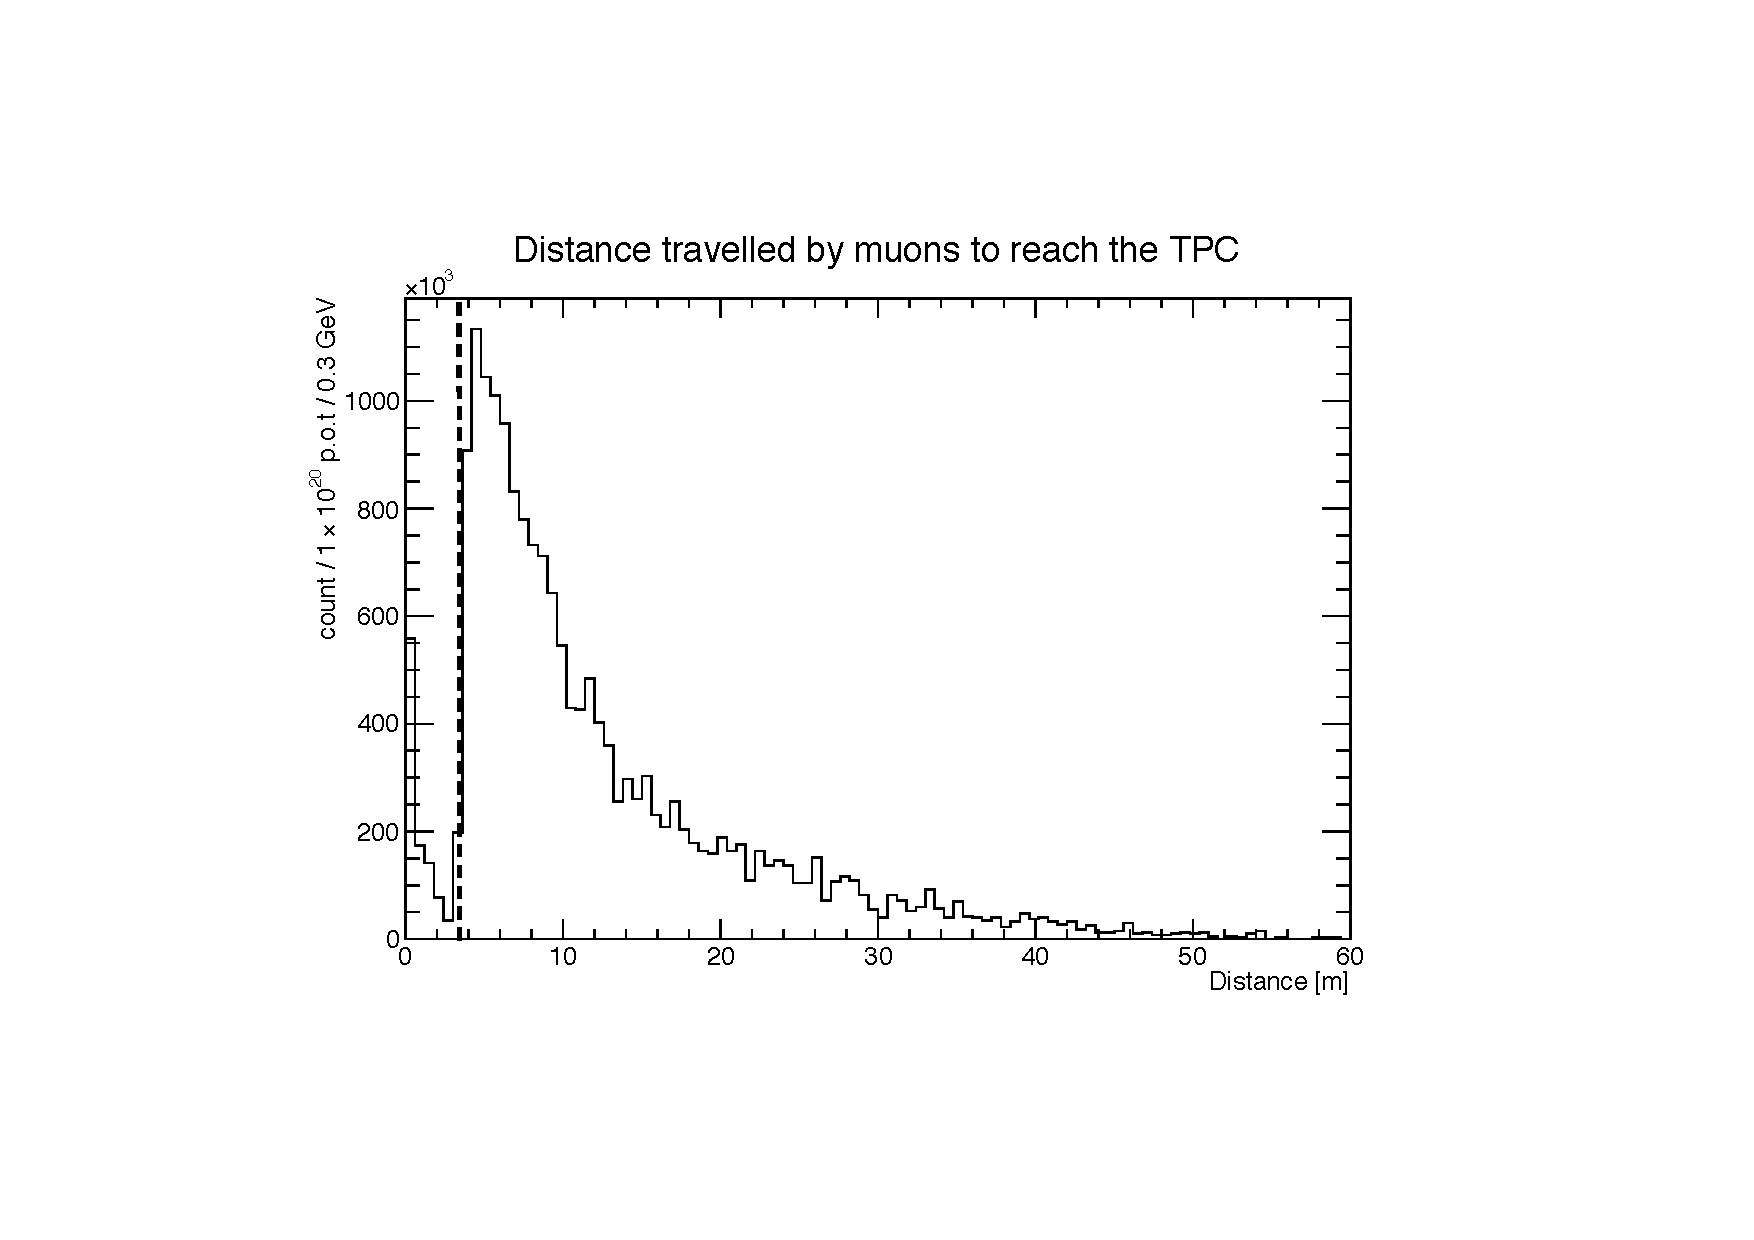
\includegraphics[width=100mm]{Chapter4/figures/rockMuonRange.pdf}
	\caption{The distance travelled by muons to reach the TPC originating from neutrino interactions outside the TPC. Showing only the magnitude of the distance travelled until the TPC is reached, and therefore does not represent their true range, as the distance after leaving the TPC is excluded. The dashed line at 3.5 m indicates the edge of the cavity and distances greater than this represent muons originating from the rock only.}
	\label{fig:rockMuonsRange}
\end{center}
\end{figure}
\begin{figure}[htbp]
\begin{center}
  	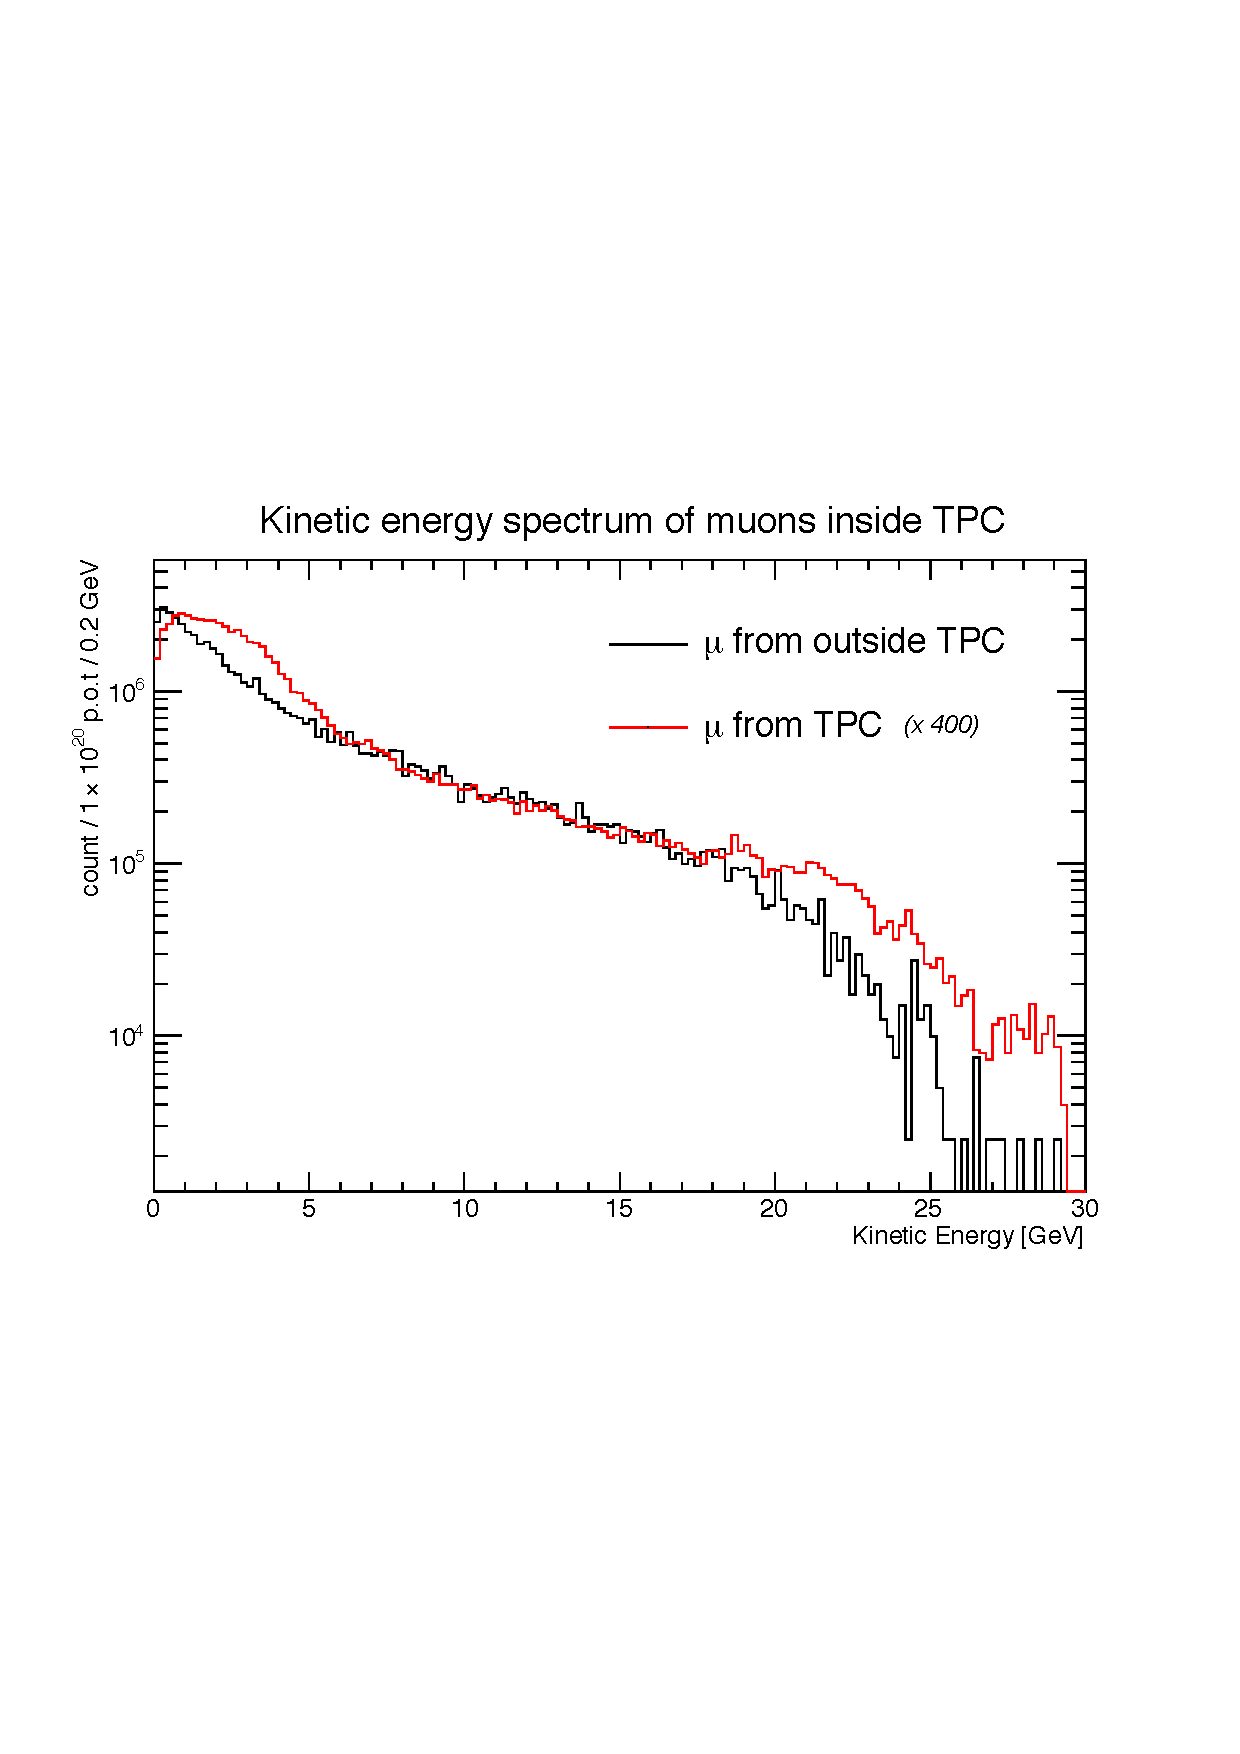
\includegraphics[width=100mm]{Chapter4/figures/muonKinEnergy_tpcAndRock.pdf}
	\caption{The kinetic energy spectrum of the muons reaching the TPC from neutrino interactions within the rock and surrounding detector components in black and those that are generated in the TPC in red. With a larger muon rate due to interactions outside the TPC the muon rate from inside the TPC is scaled by a factor of 400. After the scale factor both are normalised to 1 $\times$ 10$^{20}$ p.o.t.}
	\label{fig:rockMuonEnergy}
\end{center}
\end{figure}

Other particle types, with kinetic energies greater than 1 MeV, reaching the TPC are shown with their corresponding rates in table \ref{tab:inFluxParticles}. Figure \ref{fig:rockInteractionsOrigin} shows the original vertex position of the neutrino interaction for all secondary particles that reached the TPC. These results do not show subsequent interactions in the TPC but show any possible particle that reaches the TPC.
\begin{table}[htbp]
\centering
\begin{tabular}{ccc}
	\hline
	 \textbf{Particle Type} & \textbf{Rate [ppp]} & \textbf{\%} \\
	 \hline
	 Photons & 125.0 $\pm$ 0.9 & 40.8\\
	 Muons & 44.5 $\pm$ 0.5 & 14.5\\
	 Electrons & 24.7 $\pm$ 0.4 & 8.1\\
	 Neutrons & 21.0 $\pm$ 0.4 & 6.9\\
	 Charged Pions & 6.0 $\pm$ 0.2 & 2.0\\
	 Protons & 4.2 $\pm$ 0.2 & 1.4\\
	 Other & 13.4 $\pm$ 0.3 & 4.3\\
	 \hline
	 Neutrinos & 67.2 $\pm$ 0.6 & 22.0 \\
	 \hline
	 \hline
	 Total & 306 $\pm$ 1 & 100 \\
	\hline
\end{tabular}
\caption{Particle types of interest reaching the TPC with kinetic energies above 1 MeV. Note that the majority of the photons ($>$99\%) leaving the TPC originate from $\pi^{0}$ decays and are low energy ($<$1 GeV). Errors indicate statistical $\pm$1 $\sigma$ only.}
\label{tab:inFluxParticles}
\end{table}

\begin{figure}
\begin{center}
  	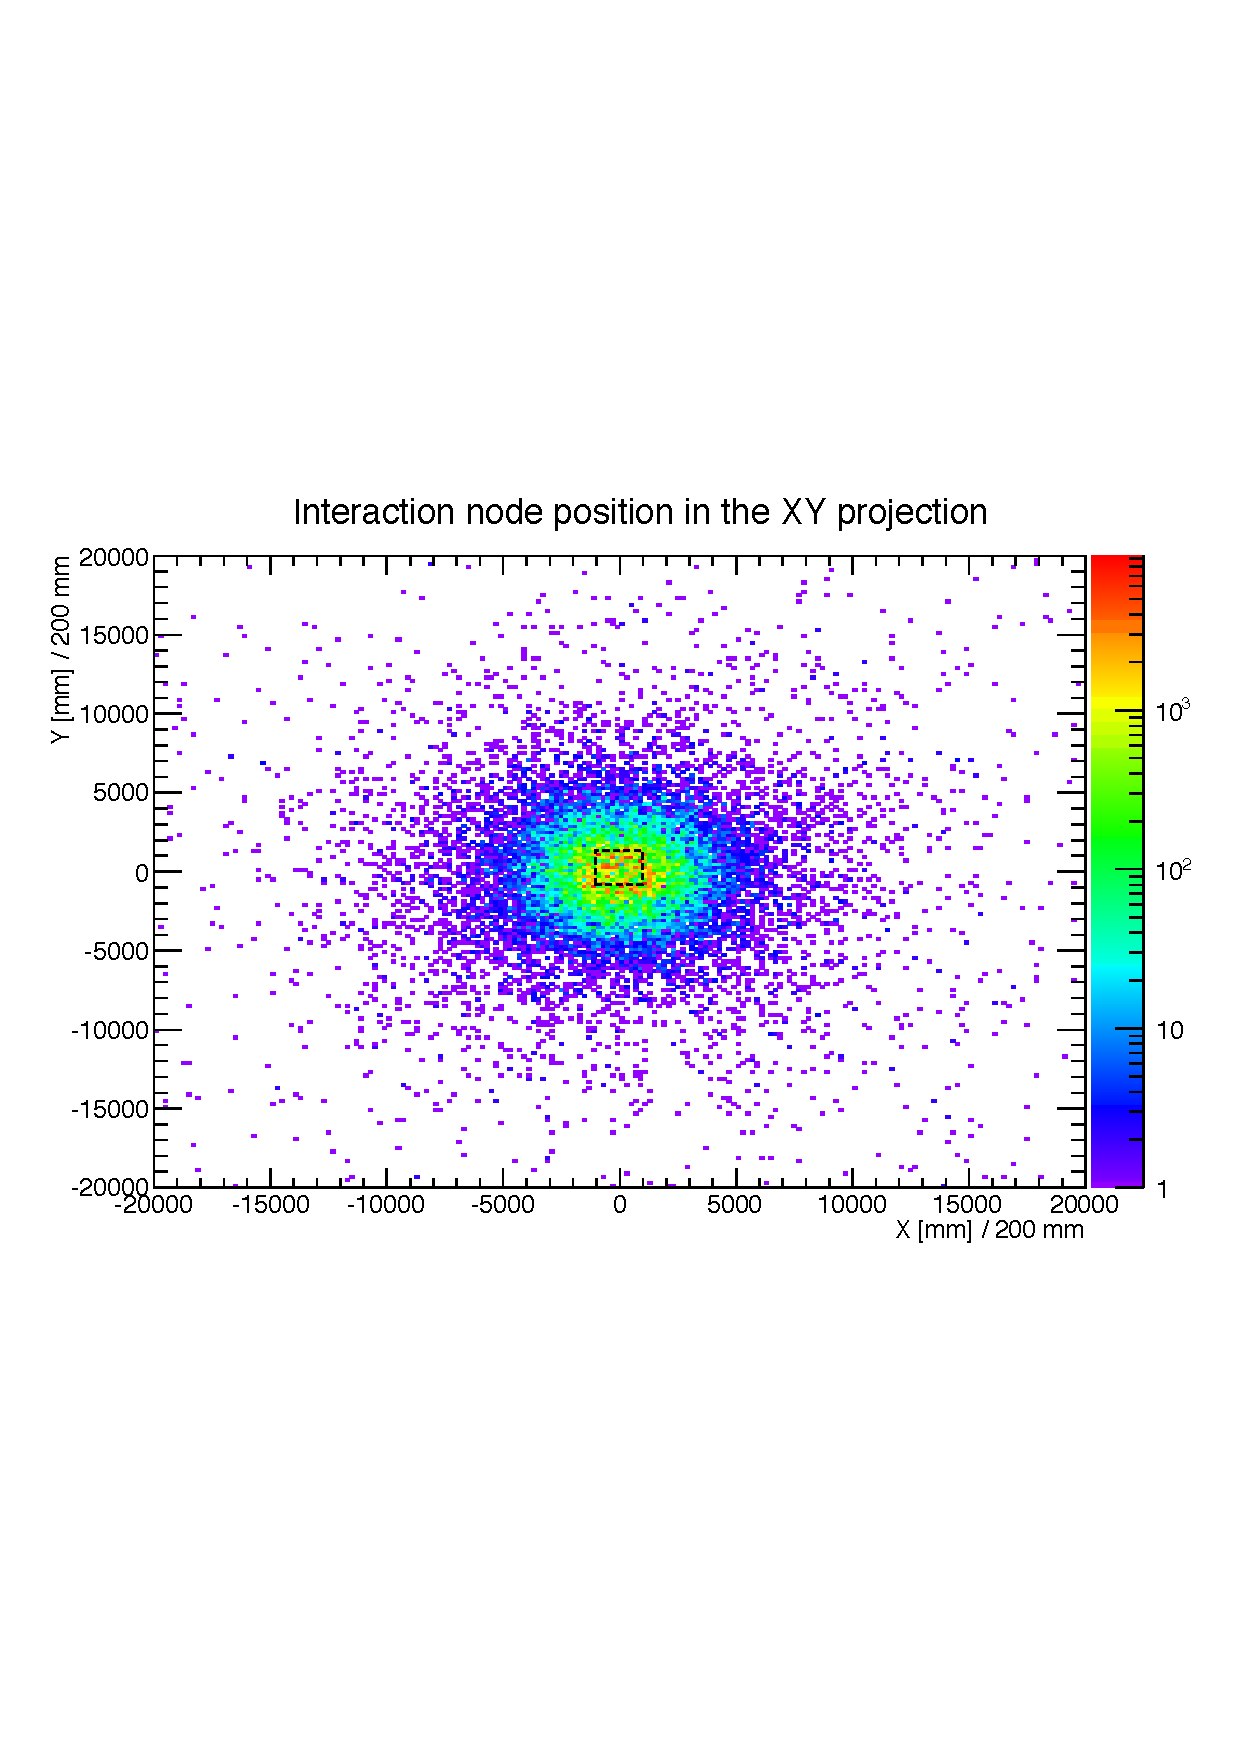
\includegraphics[width=100mm]{Chapter4/figures/rockPositionOrigin_XY_copy.pdf}\\
  	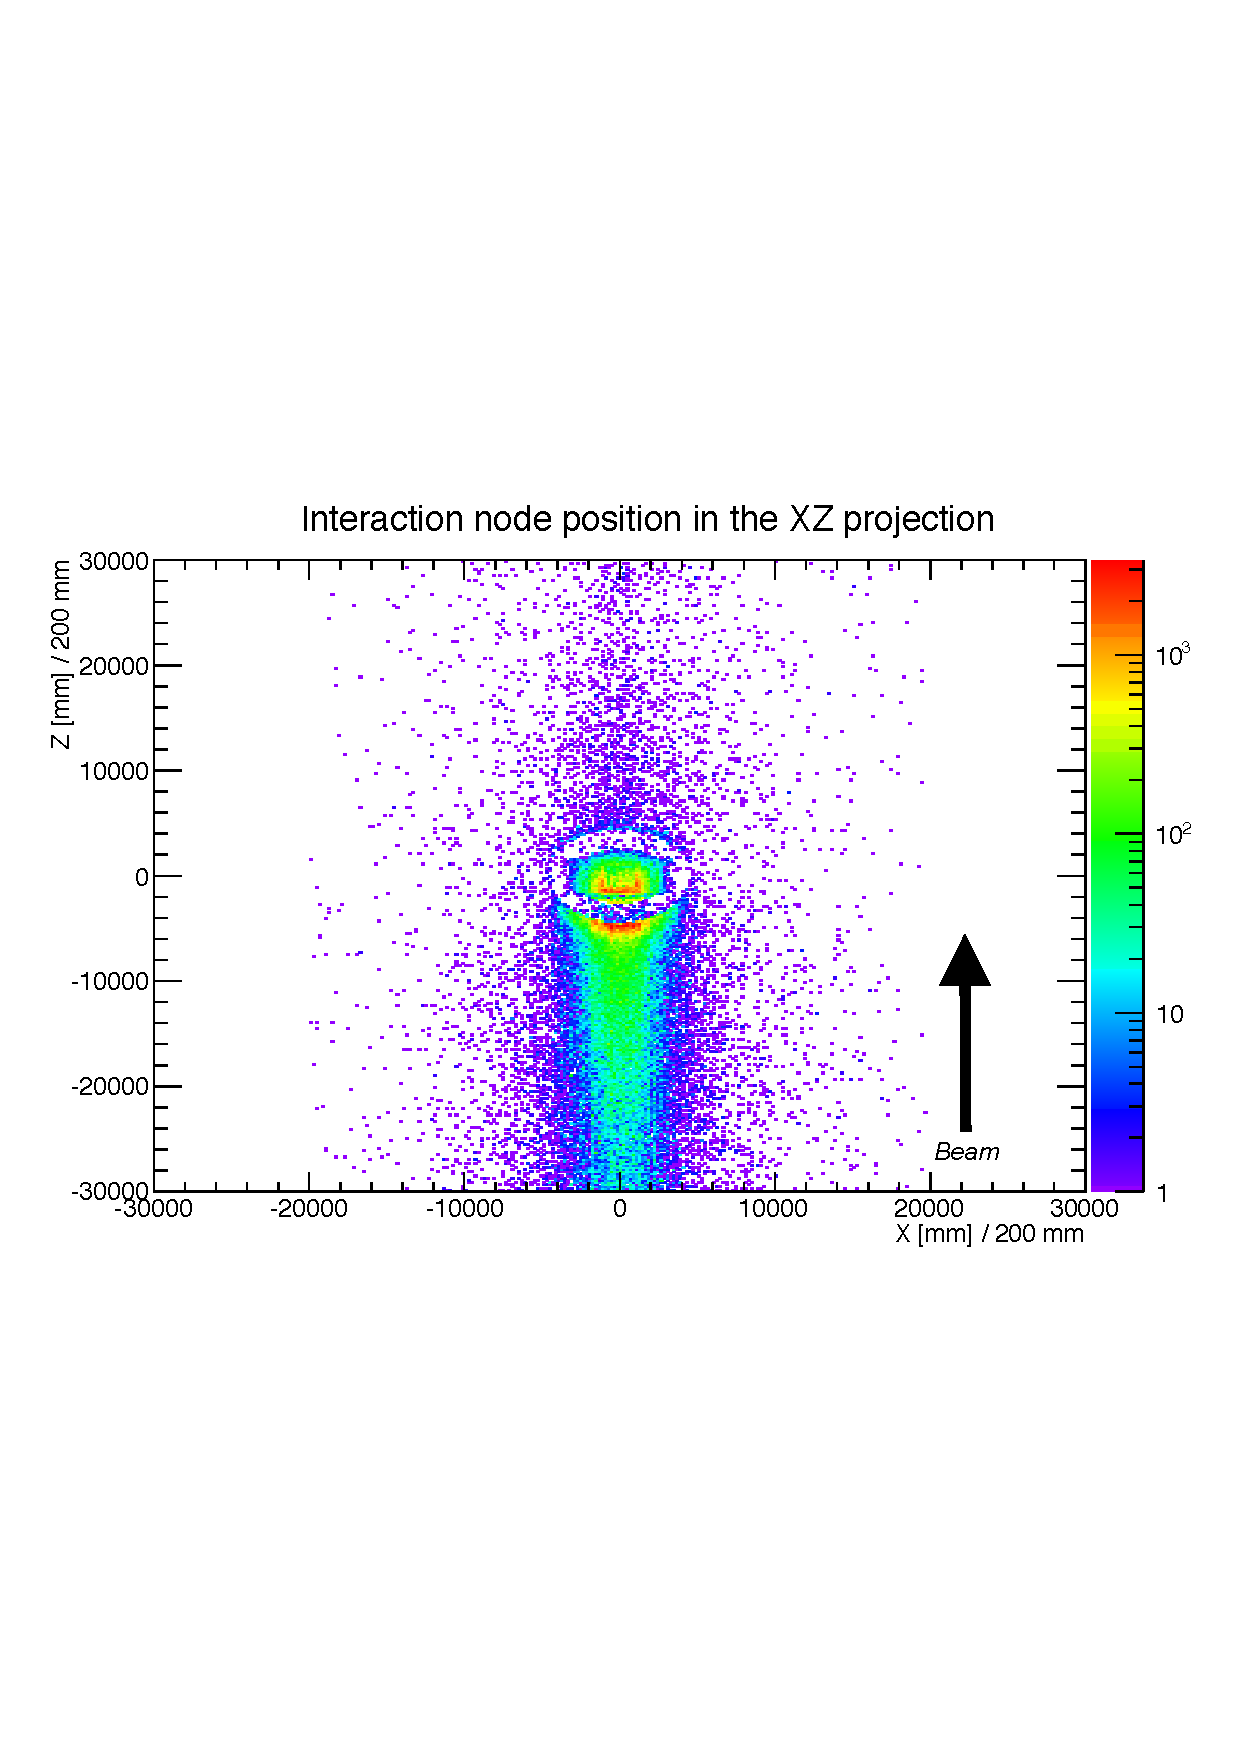
\includegraphics[width=100mm]{Chapter4/figures/rockPositionOrigin_XZ_copy.pdf}\\
  	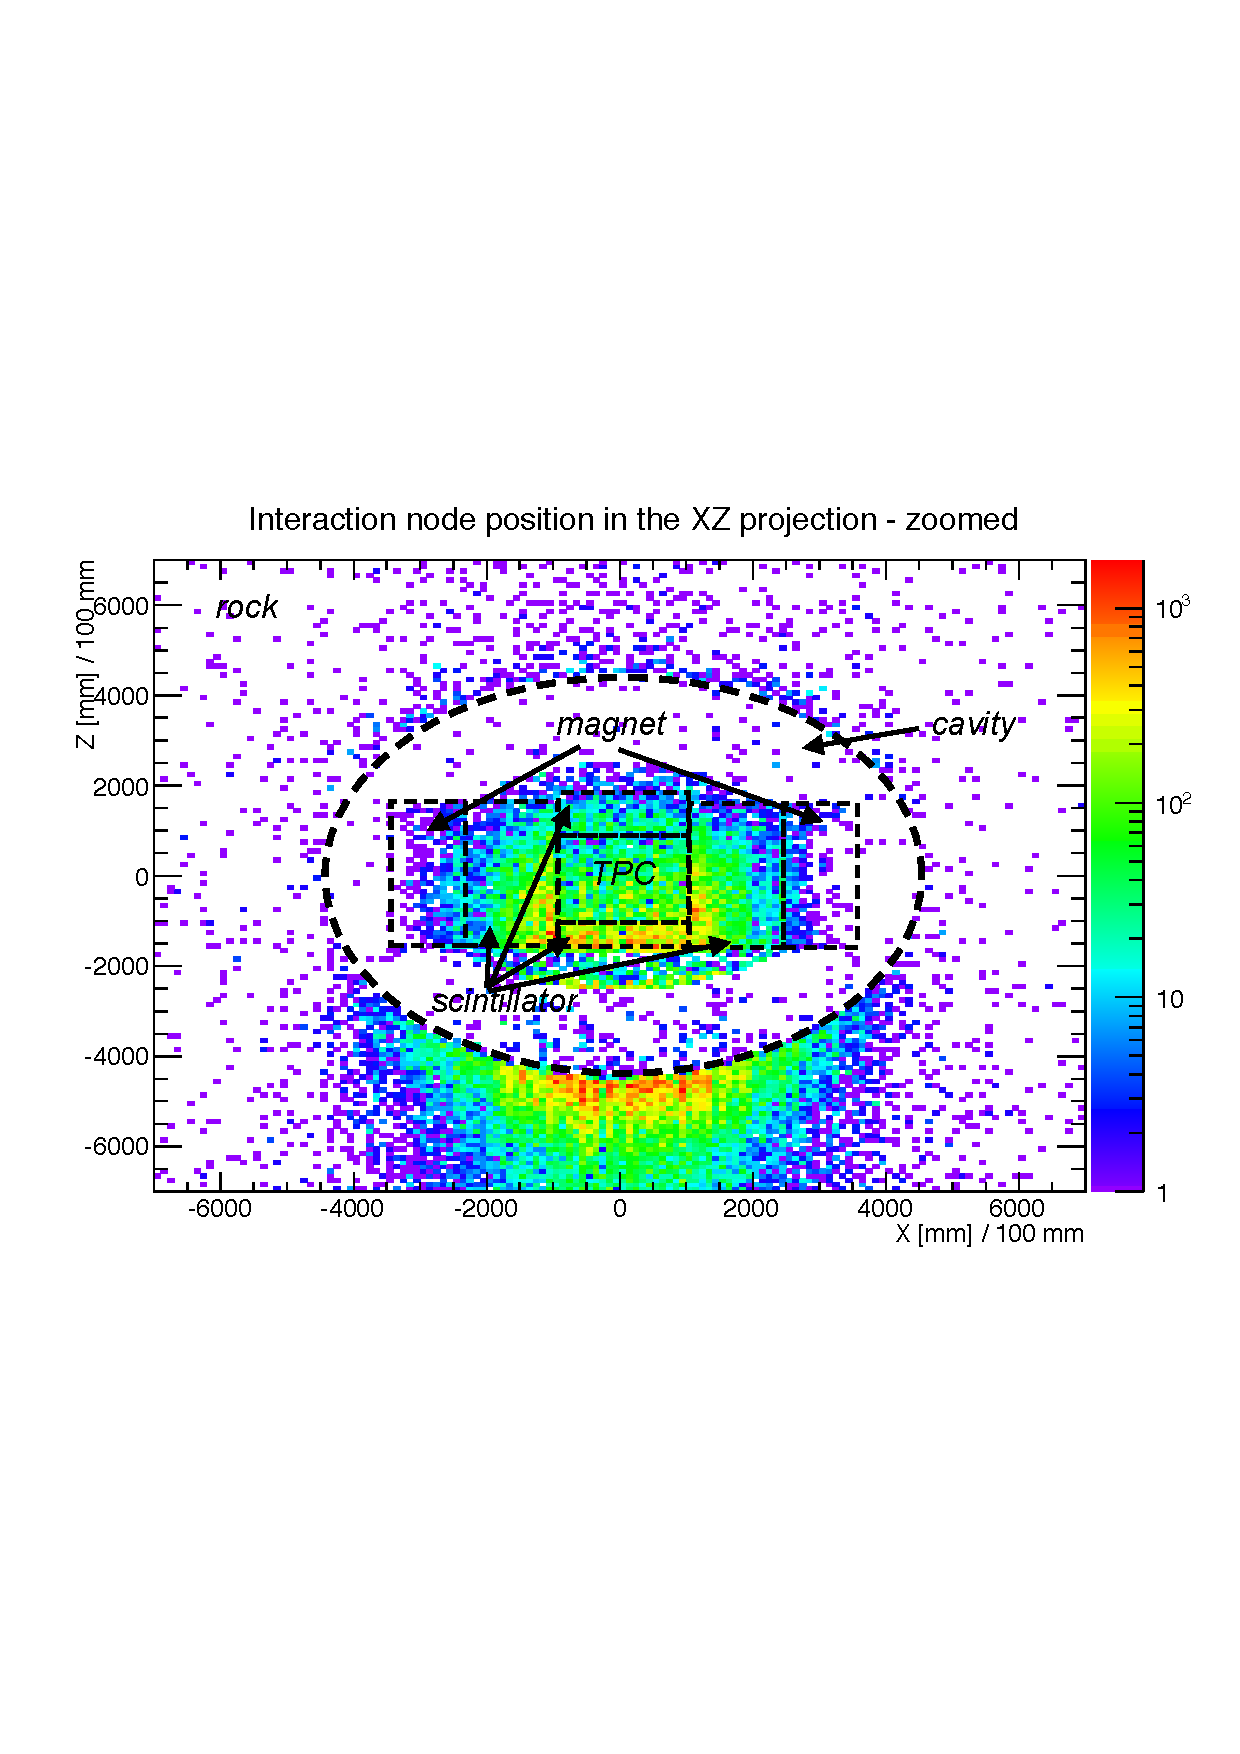
\includegraphics[width=100mm]{Chapter4/figures/rockPositionOrigin_XZ_zoom_copy1.pdf}
	\caption{Upper: The XY projection (beam into page) of the node positions of the original neutrino interaction for which a secondary reached the TPC (highlighted by the dashed line). Middle: The XZ projection (beam upwards) of the node positions of the original neutrino interaction for which a secondary reached the TPC. Lower: A zoomed in version of the middle plot to illustrate the various detector components with respect to the node positions. Counts are normalised to 4 $\times$ 10$^{16}$ p.o.t.}
	\label{fig:rockInteractionsOrigin}
\end{center}
\end{figure}

The majority of the particles arriving at the TPC originate from the surrounding rock at 75.6\%. A considerable amount also arise from neutrino interactions within the scintillator layers at 20.1\%. The rock level is irreducible but removal of some scintillator layers, especially upstream of the TPC, could decrease the background muon rate at a cost to the energy reconstruction of photons. Other detector layers and environment surroundings show their contributions in addition to the rock and scintillator layers in table \ref{tab:backgroundInteractionNodes}.

\begin{table}[htbp]
\centering
\begin{tabular}{cc}
	\hline
	 \textbf{Detector/Environment Node} & \textbf{Contribution (\%)}\\
	 \hline
	 Cavity & <0.1\\
	TPC & 0.1\\
	Inner Vessel (GAr) & 0.4 \\
	Magnet & 1.5 \\
	Vessel & 2.3 \\
	Scintillator & 20.1\\
	Rock & 75.6 \\
	\hline
\end{tabular}
\caption{All the detector/environment nodes in the geometry with their contributing percentages to secondary particles reaching the TPC where the neutrino interaction occurred originally.}
\label{tab:backgroundInteractionNodes}
\end{table}

\subsection{Muons Originating from the Beam}
The rate of muons originating from the beam, decay pipe and focusing horns has been estimated by the LAGUNA-LBNO beam group independently to be 2.5 $\mu$/m$^{2}$/10$^{13}$ p.o.t (400 GeV PF) at 800 m from the beam target \cite{lbnoInternal}. Extrapolating this value to an area of 4 m$^{2}$ for the TPC ppp yields 70 $\mu$ ppp. This is $\sim$1.6 times larger than the muons originating from the rock and detector surroundings. Estimates for the remaining beam options have not been considered by the LAGUNA beam group.

\subsection{Total Muons Expected in the TPC}
Referring back to figure \ref{fig:particleBackgrounds} it was shown there are 4 possible areas for muons to reach the TPC. Values have been calculated/estimated for all 4 areas of concern and are summarised in table \ref{tab:muonRates}. The total muon flux in the TPC is then 114.6 $\pm$ 0.8 $\mu$ ppp. Areas 1 and 3 can be controlled to some extent by ND design but areas 2 and 4 are irreducible from the ND design aspect. The latter are of course the largest contributing factors to the muon rates at 112.1 $\mu$ ppp (97.8\% of the total contribution) and therefore a reduction in areas 1 and 3 will not dramatically increase the performance.

\begin{table}[htbp]
\centering
\begin{tabular}{ccc}
	\hline
	 \textbf{Muon origin} & \textbf{Rate [ppp]}& \textbf{Contribution [\%]}\\
	 \hline
	 $\nu$ interactions in TPC & 0.1254 $\pm$ 0.0003 & 0.1\\
	 $\nu$ interactions in outer detector + cavity & 2.4 $\pm$ 0.1 & 2.1\\
	 $\nu$ interactions in rock & 42.1 $\pm$ 0.5 & 36.7 \\
	 Beam + decay pipe + horns & 70 & 61.1 \\
	\hline
	\textbf{Total} & \textbf{114.6} $\boldsymbol{\pm}$ \textbf{0.8} & \textbf{100}\\
	\hline
\end{tabular}
\caption{A table showing the four main sources of muons reaching the TPC with their associated rates determined from simulations. These numbers are translated into how much each contributes to the total of the four origins. All values are based on the 400 GeV PF beam option. Uncertainties indicate 1 $\sigma$ statistical errors only.}
\label{tab:muonRates}
\end{table}

To estimate if pile up is an issue the number of muon tracks in the TPC per unit area (2 $\times$ 2 m$^{2}$) shows that $\sim$14 $\mu$ tracks/m$^{2}$/spill will pass through the TPC. With each spill extraction lasting 10.5 $\mu$s this results in $\sim$1-2 $\mu$ tracks/m$^{2}$/$\mu$s. With drift times of $\sim$100 $\mu$s detector pile up is therefore unavoidable. However if the vertex can be resolved then it can help discriminate between the tracks within the TPC. At $\sim$1 $\mu$ track/700 cm$^{2}$/spill the vertex should be easily resolved.

\section{Particles Leaving the TPC}
It is important for other stages of the ND design to realise what particles leave the TPC. This primarily concerns the angular distribution of photons and their associated energy spectrum, as the majority of these photons will originate from $\pi^{0}$s. Figure \ref{fig:particleFluxOutTPC} shows the kinetic energies as a function of angular dependance for particles of key concern. 

\begin{figure}[htbp]
\begin{center}
  	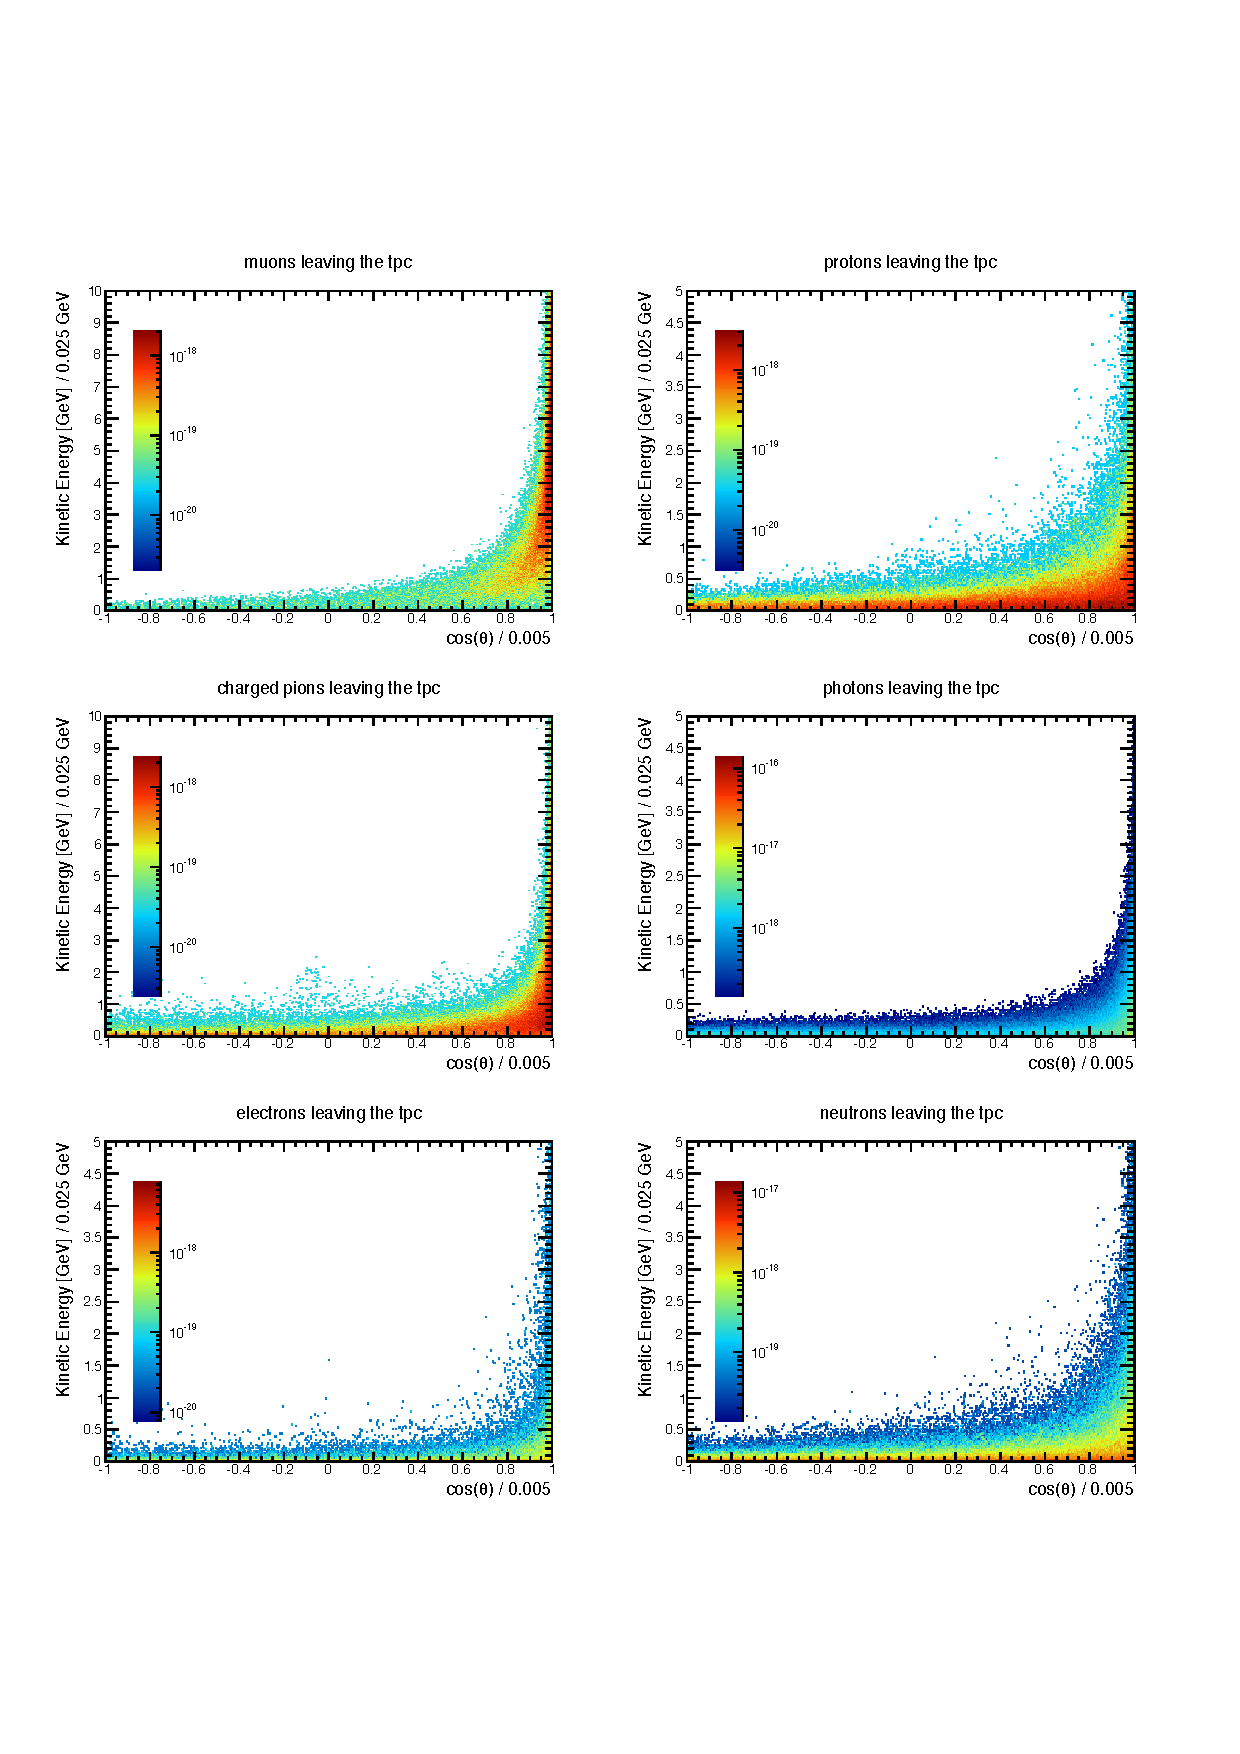
\includegraphics[width=150mm]{Chapter4/figures/particleOut_energyVsCosTheta.pdf}
	\caption{The kinetic energies of the particles of key concern leaving the TPC as a function of angular dependance. The angular dependance is measured by cos$\theta$, which is a measure of the particles momentum in the beam direction, that is cos$\theta$ = $p_{z}/|\boldsymbol{p}|$. Note the different energy scales for muons and charged pions (0-10 GeV) as they are produced with higher energies, the other scales are 0-5 GeV. Particle counts are normalised to p.o.t.}
	\label{fig:particleFluxOutTPC}
\end{center}
\end{figure}

The majority of the particles leaving the TPC are photons at 30.7\%, that is 0.5255 $\pm$ 0.0008 (stat) ppp. Table \ref{tab:particleOutTPC} shows the main particle types of concern that leave the TPC from neutrino interactions within the TPC. Given that the TPC can perform momentum measurements on protons, charged pions and muons, the two other major particle types are photons and neutrons, of which momentum measurements cannot be performed within the TPC. Outer detector layers such as the TAS will hope to tackle these particles.

\begin{table}[htbp]
\centering
\begin{tabular}{ccc}
	\hline
	 \textbf{Particle} & \textbf{Rate leaving [ppp]}& \textbf{Contribution [\%]}\\
	 \hline
	Photons & 0.5255 $\pm$ 0.0008 (stat) & 30.7 \\
	Neutrons & 0.3855 $\pm$ 0.0007 (stat) & 22.5 \\
	Protons & 0.2560 $\pm$ 0.0006 (stat) & 14.9 \\
	Charged Pions & 0.2291 $\pm$ 0.0006 (stat) & 13.4 \\
	Muons & 0.1297 $\pm$ 0.0004 (stat) & 7.6 \\
	Electrons & 0.0585 $\pm$ 0.0002 (stat) & 3.4 \\
	Neutrinos & 0.0580 $\pm$ 0.0002 (stat) & 3.4 \\
	Other & 0.0708 $\pm$ 0.0002 (stat) & 4.1\\
	\hline
\end{tabular}
\caption{The particle types arising from neutrino interactions in the TPC that then subsequently leave the TPC boundaries. Their associated rates at which they do so is shown per proton pulse (ppp) with their contribution to the total number of particles leaving the TPC. Rates correspond to all particles with kinetic energies in excess of 1 MeV.}
\label{tab:particleOutTPC}
\end{table}

%\section{Neutrino Energy Reconstruction}
%Two important requirements of the ND are to measure the neutrino flux and perform cross sectional measurements. Both of these demand an accurate measurement of the incident neutrino energy such that the neutrino spectrum can be determined as a function of energy. Estimation of the ND performance with respect to neutrino energy reconstruction is then of key importance for realising the physics reach and ultimately the accuracy of neutrino oscillation measurements. A study focused on the neutrino energy reconstruction within the ND is performed within the remainder of this chapter using the TPC and the TAS sub detector capabilities. The aim of this study is to quantitatively provide initial estimates on the NDs ability to reconstruct the neutrino energy, providing an upper bound to what can be expected for a realisation of the ND.
%
%\subsection{Momentum Reconstruction Techniques in the TPC}
%Detector hits are recorded for all particles that deposit energy in the TPC. A track is defined as a collection of detector hits that originate from an interaction of a single particle. Translating hits into tracks is done by matching the track identification numbers, which are unique to each secondary particle, to the detector hit. Once sorted into tracks only primary particles, that is FSPL and FSS from the neutrino interaction, are recorded in the TPC.
%
%By measurement of the track length and the sagitta the transverse momentum of the charged particle traversing the TPC can be approximated by equation \ref{eq:momMeasurements}, which follows from the earlier equation \ref{eq:magFieldSagitta}. Here the transverse momentum, $p^{trans}$ = $\sqrt{p_{y}^{2} + p_{z}^{2}}$ as the magnetic field, $\boldsymbol{B}$ = (0.5 T, 0, 0), is perpendicular to the beam direction, (0, 0, 1).
%\begin{equation}
%	p^{trans} [\textnormal{GeV/c}] = \frac{B_{z}[\textnormal{T}]l^{2}[\textnormal{m}^{2}]}{26.7s[\textnormal{m}]}
%	\label{eq:momMeasurements}
%\end{equation}
%
%The measurement of the track length is determined by the position of the initial and final truth detector hits in the TPC, $\boldsymbol{X^{i}}$ = ($X^{i}_{x}$, $X^{i}_{y}$,$X^{i}_{z}$) and $\boldsymbol{X^{f}}$ = ($X^{f}_{x}$, $X^{f}_{y}$,$X^{f}_{z}$) respectively, as $l$ = $|\boldsymbol{X^{f}}$ - $\boldsymbol{X^{i}}|$. No smearing on the position is performed and truth values are used for determination of the track length.
%
%Measurement of the sagitta is done via a smearing technique. An initial value is determined by finding the hit on the track which minimises the distance between the hit and the midpoint of the line between the initial and final points, $\boldsymbol{X^{mid}}$ = ($\boldsymbol{X^{i}}$ + $\boldsymbol{X^{f}}$)/2. The minimum distance is then taken as the initial sagitta, $s_{0}$. Figure \ref{fig:trackAndHitsDrawing} shows the process, with the detector hits as red dots, the initial and final points as blue dots and the midpoint as a black dot. This result is then smeared using a Gaussian distribution of mean value, $\bar{x}$ = $s_{0}$ and $\sigma$ = $\delta$$s$ = 300 $\mu$m (T2K ND280 value). To smear the sagitta is the process of selecting a random number (TRandom3 in ROOT [ref here]) from the Gaussian distribution to return a new smeared value of the sagitta, $s$.

%Measurement of the sagitta is done via a smearing technique. No track reconstruction is performed within the software and hence no measurement of the sagitta can be made. However a smeared sagitta value is determined by the following steps:
%
%\begin{enumerate}
%	\item Determine the truth transverse momentum $p_{truth}^{trans} = \sqrt{p_{y}^{2} + p_{z}^{2}}$ from the initial hit in TPC
%	\item Calculate the truth sagitta $s_{truth} = Bl^{2}/26.7p_{truth}^{trans}$
%	\item Apply Gaussian distribution with mean value $\bar{x}_{s} = s_{truth}$ and width $\sigma_{s}$ = $\delta$$s$ = 300 $\mu$m (T2K ND280 value)
%	\item Using random number generator (TRandom3 from ROOT) pull variable $s_{smear}$ from distribution
%	\item Reconstruct transverse momentum $p_{recon}^{trans} = Bl^{2}/26.7s_{smear}$
%	%\item Spread of transverse momentum  $\delta p_{recon}^{trans}$ =  $p_{recon}^{trans}\sigma_{s}/s_{smear}$
%\end{enumerate}
%
%%\begin{figure}[htbp]
%%\begin{center}
%%  	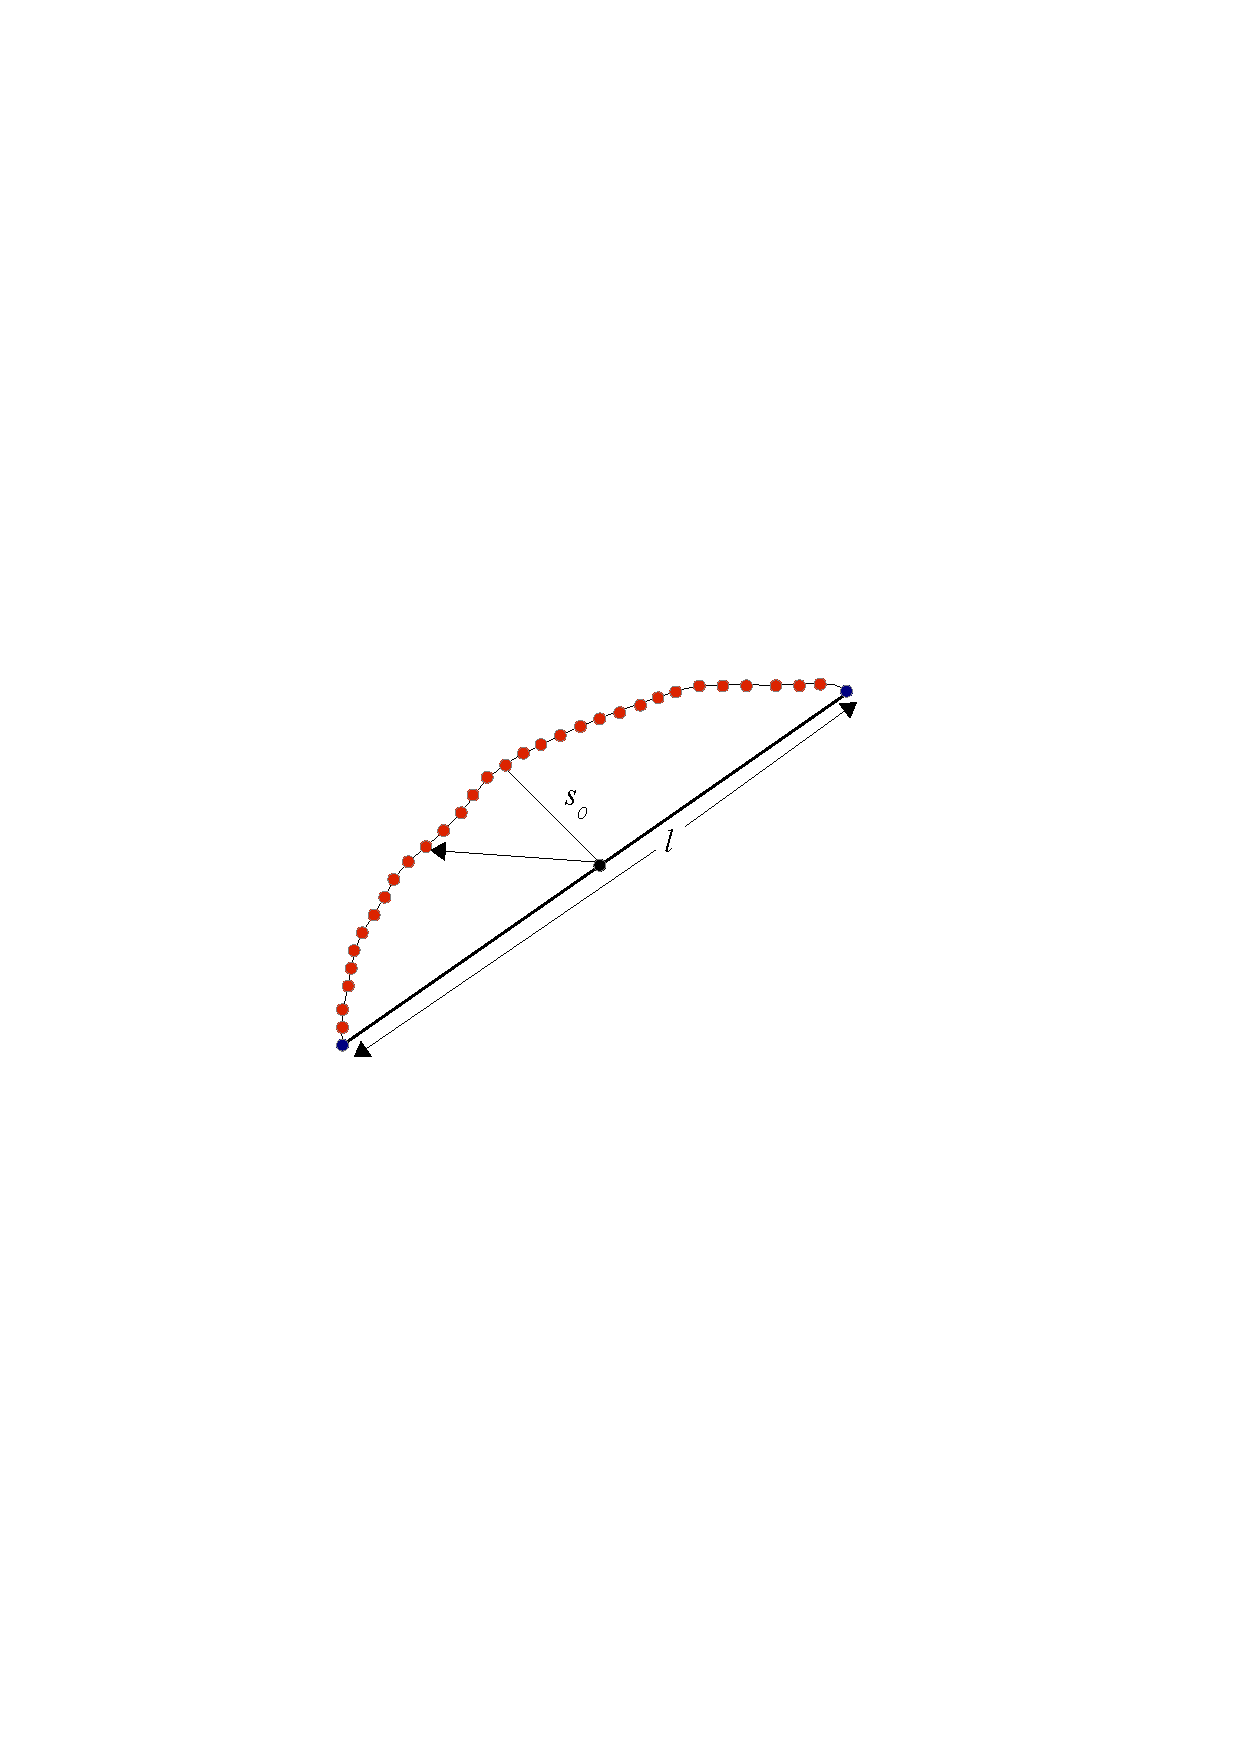
\includegraphics[width=90mm]{Chapter4/figures/trackAndHitsDrawing.pdf}
%%	\caption{A drawing to represent a track traversing the TPC in a magnetic field. Detector hits are in red, which mark points of ionisation and truth values are taken at each of these points. The blue dots represent the initial and final points in the TPC with the black point showing the midpoint position, $\boldsymbol{X^{mid}}$.}
%%	\label{fig:trackAndHitsDrawing}
%%\end{center}
%%\end{figure}
%
%A fiducial cut of 20 cm is applied to the TPC so that neutrino vertices that fall within 20 cm of the TPC boundaries are rejected for reconstruction, that is rejection of all secondaries arising from the neutrino event. Also a minimum requirement of at least five hits per track is implemented to allow a reasonable measurement of the sagitta, however with small step lengths of 0.1 mm, the majority of the charged tracks well exceed this requirement.
%
%Reconstructing the track momentum in this way is not a full reconstruction as detector effects, electron drifting and track reconstruction are not performed. Truth values of the position, the initial transverse momentum, track PDG and identification numbers are the sole pieces of information used. Each charged track that deposited energy in the TPC with at least 5 hit points is reconstructed in this way.
%
%\subsection{Momentum Reconstruction of Muons in the TPC}
%Using truth information on the particle type and PDG code, muons are selected to see how well measurement of their transverse momentum compares to their full truth 3-momentum, $p_{truth} = \sqrt{p^{2}_{trans} + p^{2}_{x}}$. It was shown that muons are generally very forward going and hence most of their momentum is in the beam direction, so to good approximation their momentum can be taken as their transverse momentum. Figure \ref{fig:muonMomRecon} shows the comparison with the reconstructed transverse momentum as a function of truth 3-momentum.
%
%\begin{figure}[htbp]
%\begin{center}
% 	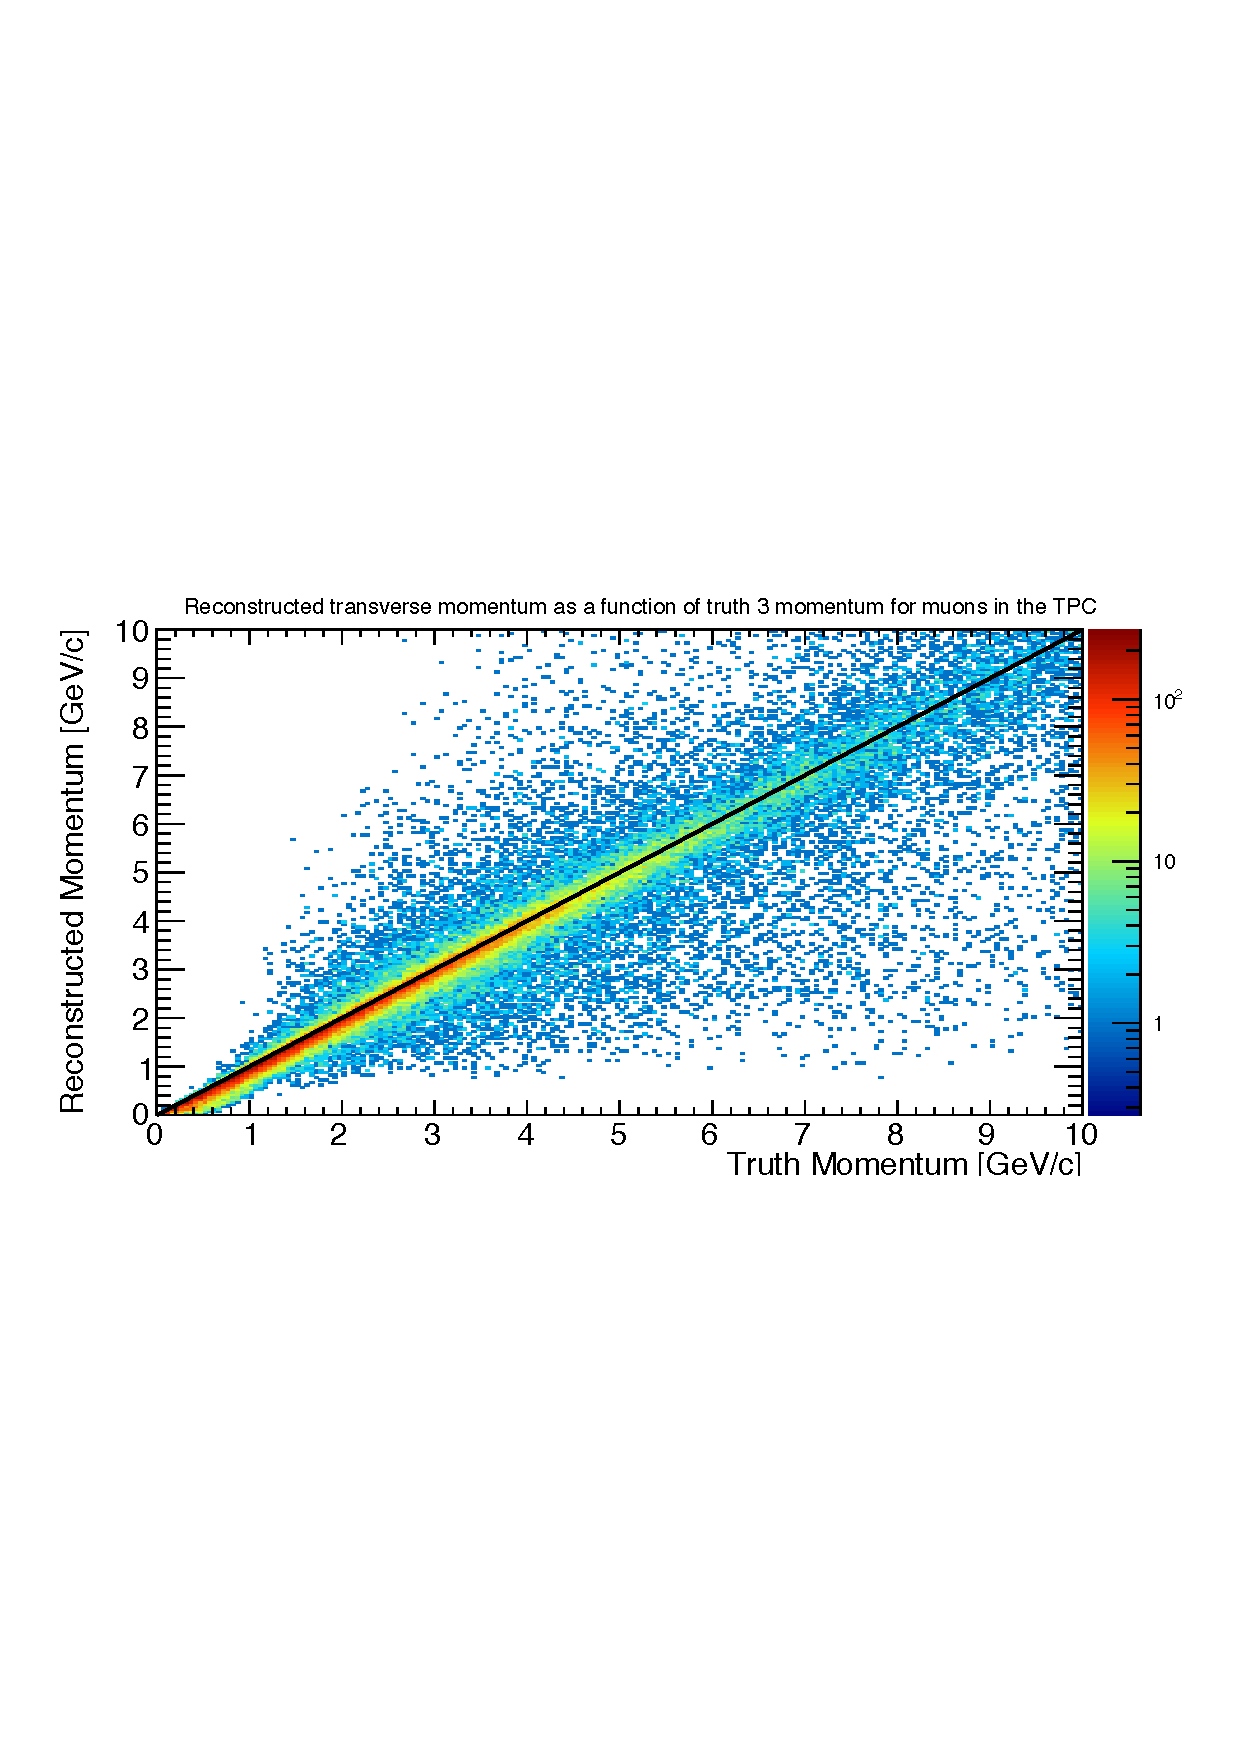
\includegraphics[width=76mm,height=55mm]{Chapter4/figures/recon_truthVsReconMom_muon.pdf}
% 	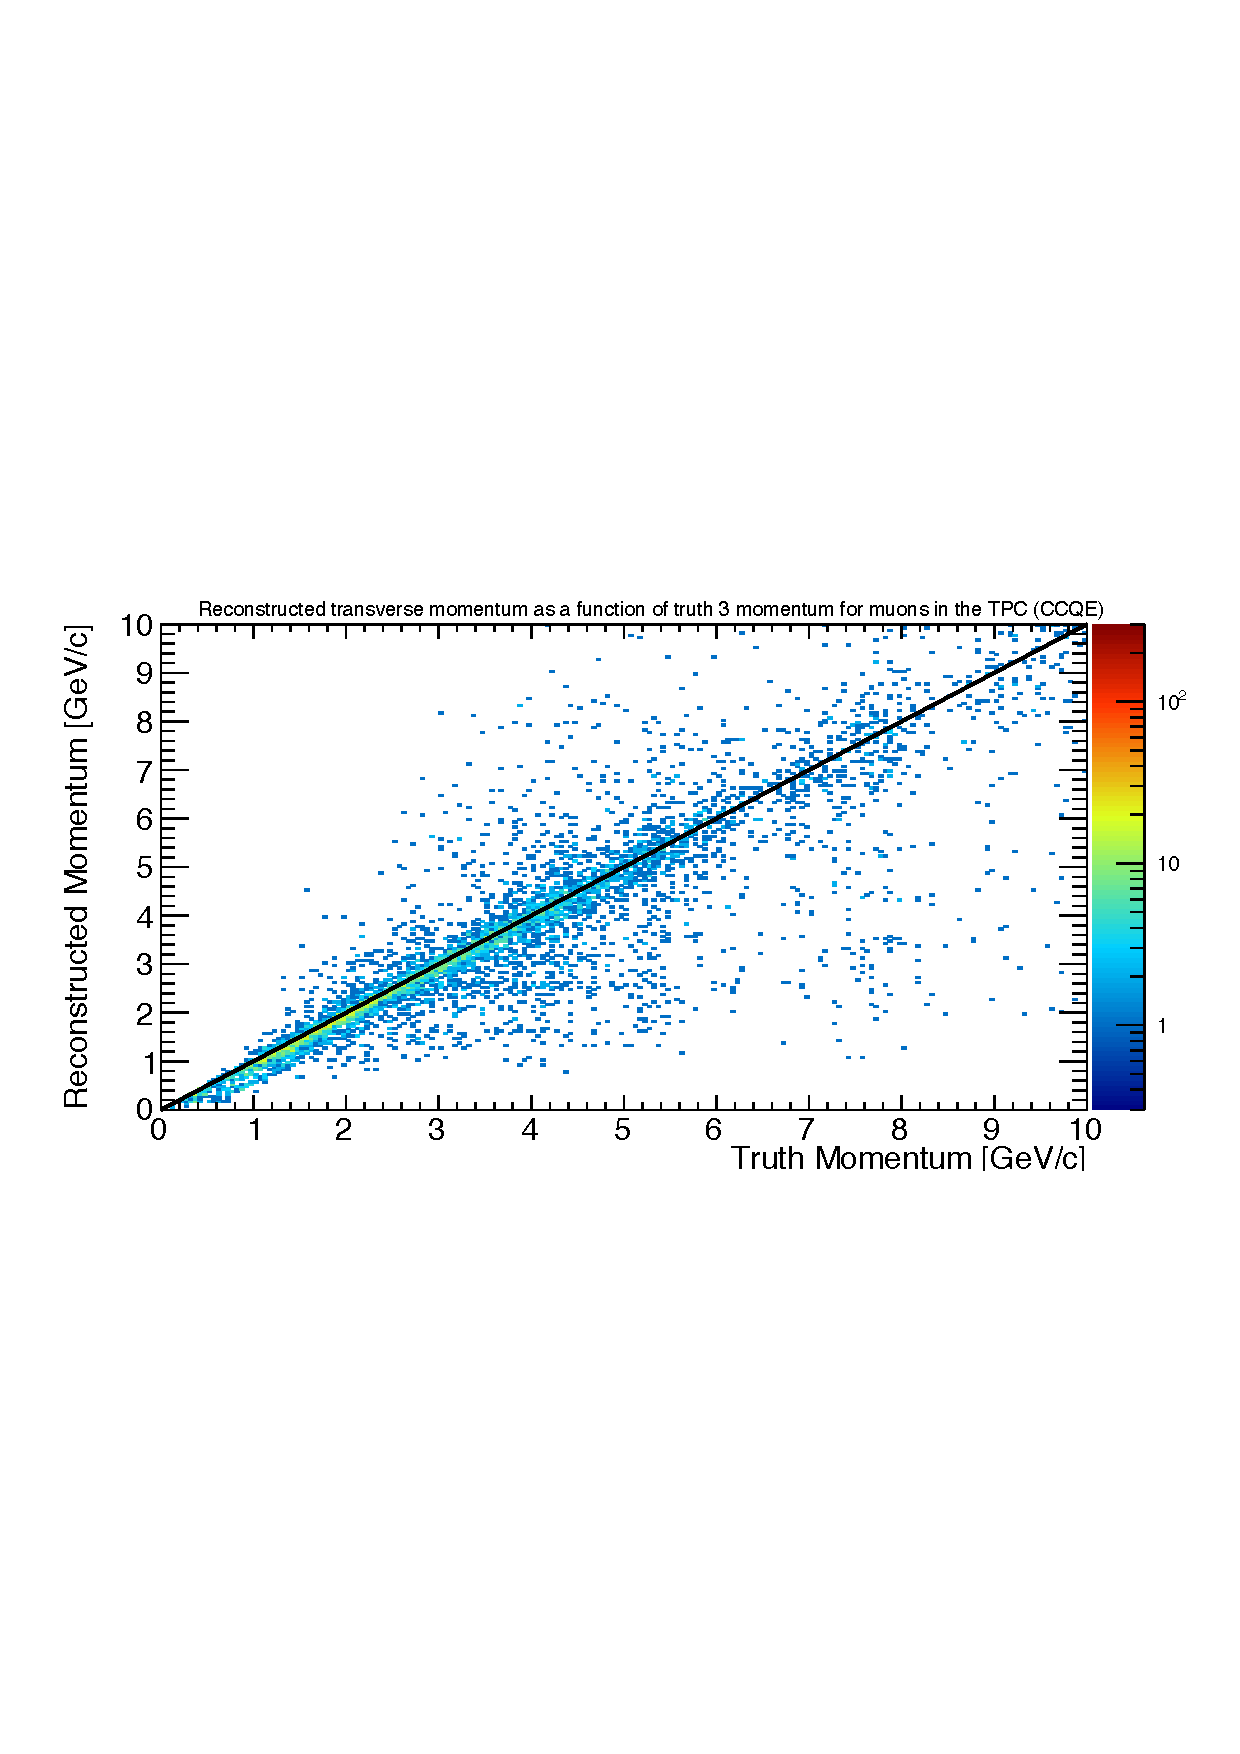
\includegraphics[width=76mm,height=55mm]{Chapter4/figures/recon_truthVsReconMom_muon_ccqe.pdf}
%	\caption{The comparison of the reconstructed transverse momentum of muons in the TPC as a function of truth 3-momentum for all neutrino interaction types (left) and CCQE only (right). Histograms are binned on an event  by event basis.}
%	\label{fig:muonMomRecon}
%\end{center}
%\end{figure}
%
%Using this technique shows very good reconstruction of muons which is important for CCQE neutrino energy reconstruction, as in the two body interaction measurement of the muons momentum yields the neutrinos energy. This however requires measurement of the angle between the muon track and neutrino beam axis, $\theta$ in equation \ref{eq:ccqeNuEnergy}. Measurement of cos$\theta$ is done by taking the first and second hit positions of the muon track, $\boldsymbol{X_{1}}$ and $\boldsymbol{X_{2}}$ respectively, and projecting this onto the beam axis, hence cos$\theta$ = ($\boldsymbol{X_{2}}$ -$\boldsymbol{X_{1}}$)$\cdot$(0,0,1). CCQE-like interactions, that is events with a muon and proton in the final state but where the interaction is actually not CCQE are not considered. Only true CCQE events are considered using truth information from GENIE.
%
%The left of figure \ref{fig:neutrinoCCQEMomRecon} shows the reconstructed neutrino momentum as a function of truth neutrino energy. A similar plot is shown on the right of the same figure which shows the mean reconstructed neutrino energy value for truth bins of 0.5 GeV, again for CCQE events only. Both representations show that very good reconstruction of the neutrino momentum can be achieved with this technique. Neutrino energies below 6 GeV follow extremely good reconstruction based on the mean value with higher energies deviating slightly from the $E_{truth} = E_{recon}$ line, due to higher momentum muons having smaller sagita values and hence larger smearing over the momentum. This is also due to lower statistics for CCQE events at higher energies, as DIS events are far more favourable at these energies.
%Generally more CCQE events are reconstructed with lower energies than the truth due to the assumption that all of the muons momentum is transverse. This can be noticed more clearly by the asymmetry of the plot in figure \ref{fig:neutrinoCCQEMomReconDiff} which shows the difference between the truth and reconstructed momentum of the neutrino $(p_{truth} - p_{recon})/p_{truth}$.
%
%\begin{figure}[htbp]
%\begin{center}
% 	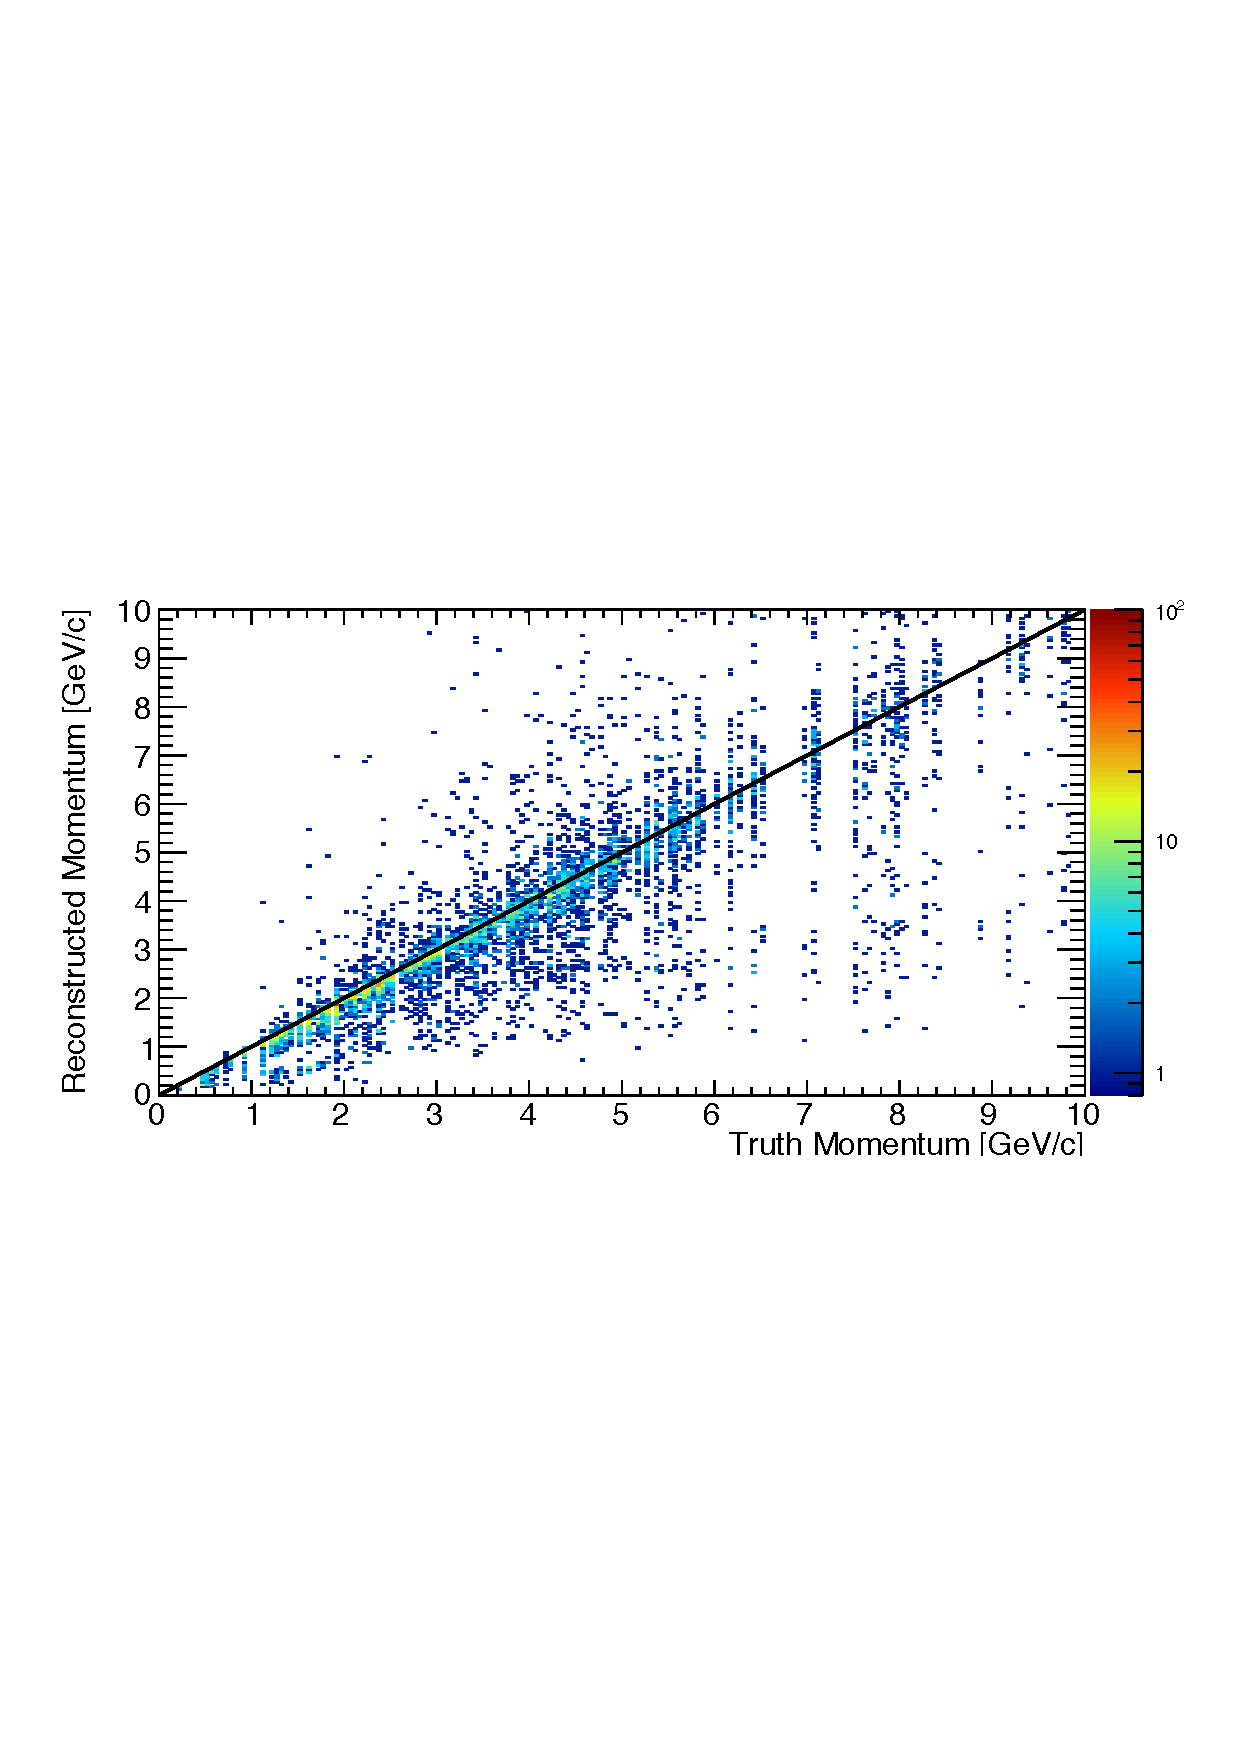
\includegraphics[width=74mm,height=50mm]{Chapter4/figures/recon_truthVsReconMom_neutrino_ccqe_v1.pdf}
%	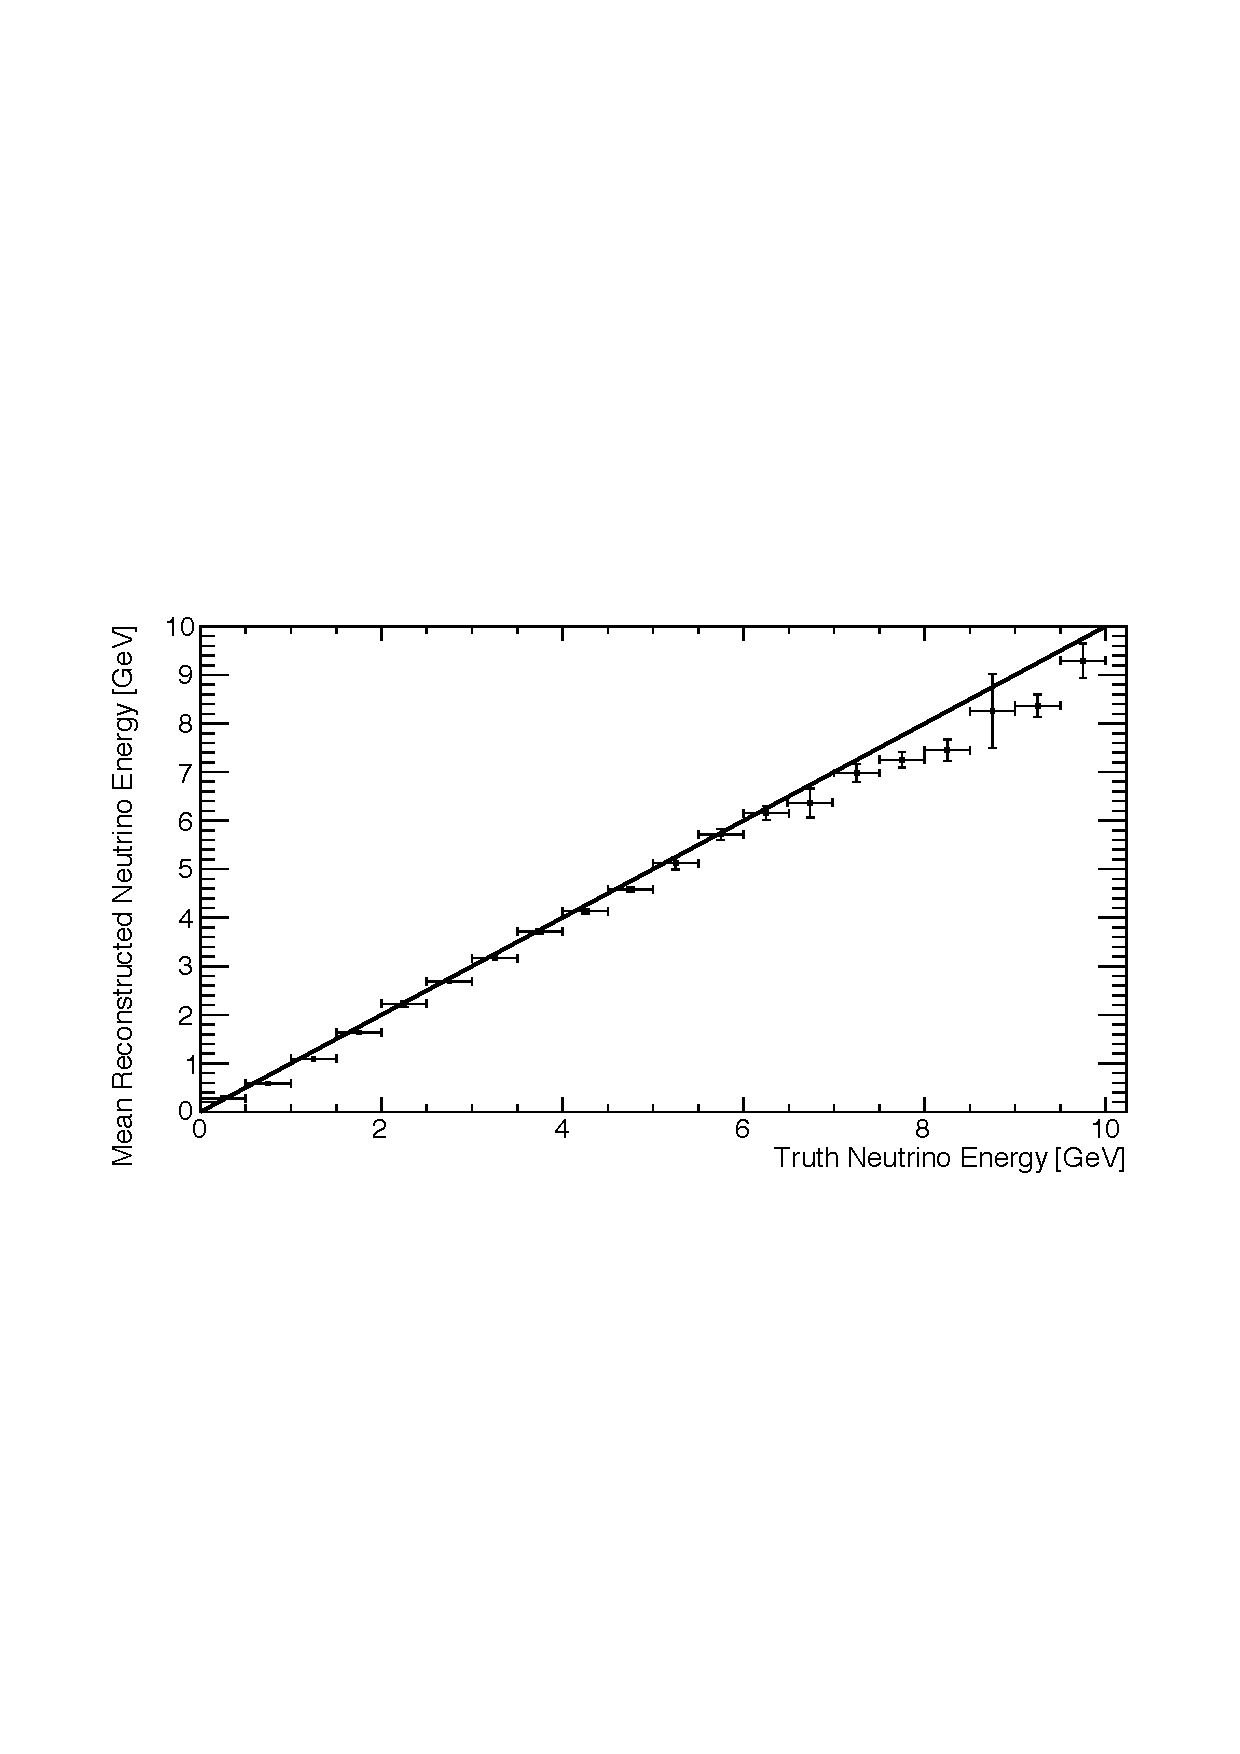
\includegraphics[width=74mm,height=48mm]{Chapter4/figures/mean_recon_neutrino_energy_ccqe.pdf}
%	\caption{Left: The reconstructed neutrino momentum as a function of the truth neutrino momentum for CCQE interactions only. Right: The mean reconstructed neutrino energy as a function of truth neutrino energy. The mean reconstructed value is determined from all events that fall within each 0.5 GeV truth bin. Error bars indicate the standard deviation value of the mean, 1$\sigma$. The neutrino momentum/energy is determined solely from the outgoing muon. Results based on simulation of exposure 9.6 $\times$ 10$^{19}$ p.o.t. }
%	\label{fig:neutrinoCCQEMomRecon}
%\end{center}
%\end{figure}
%
%\begin{figure}[htbp]
%\begin{center}
% 	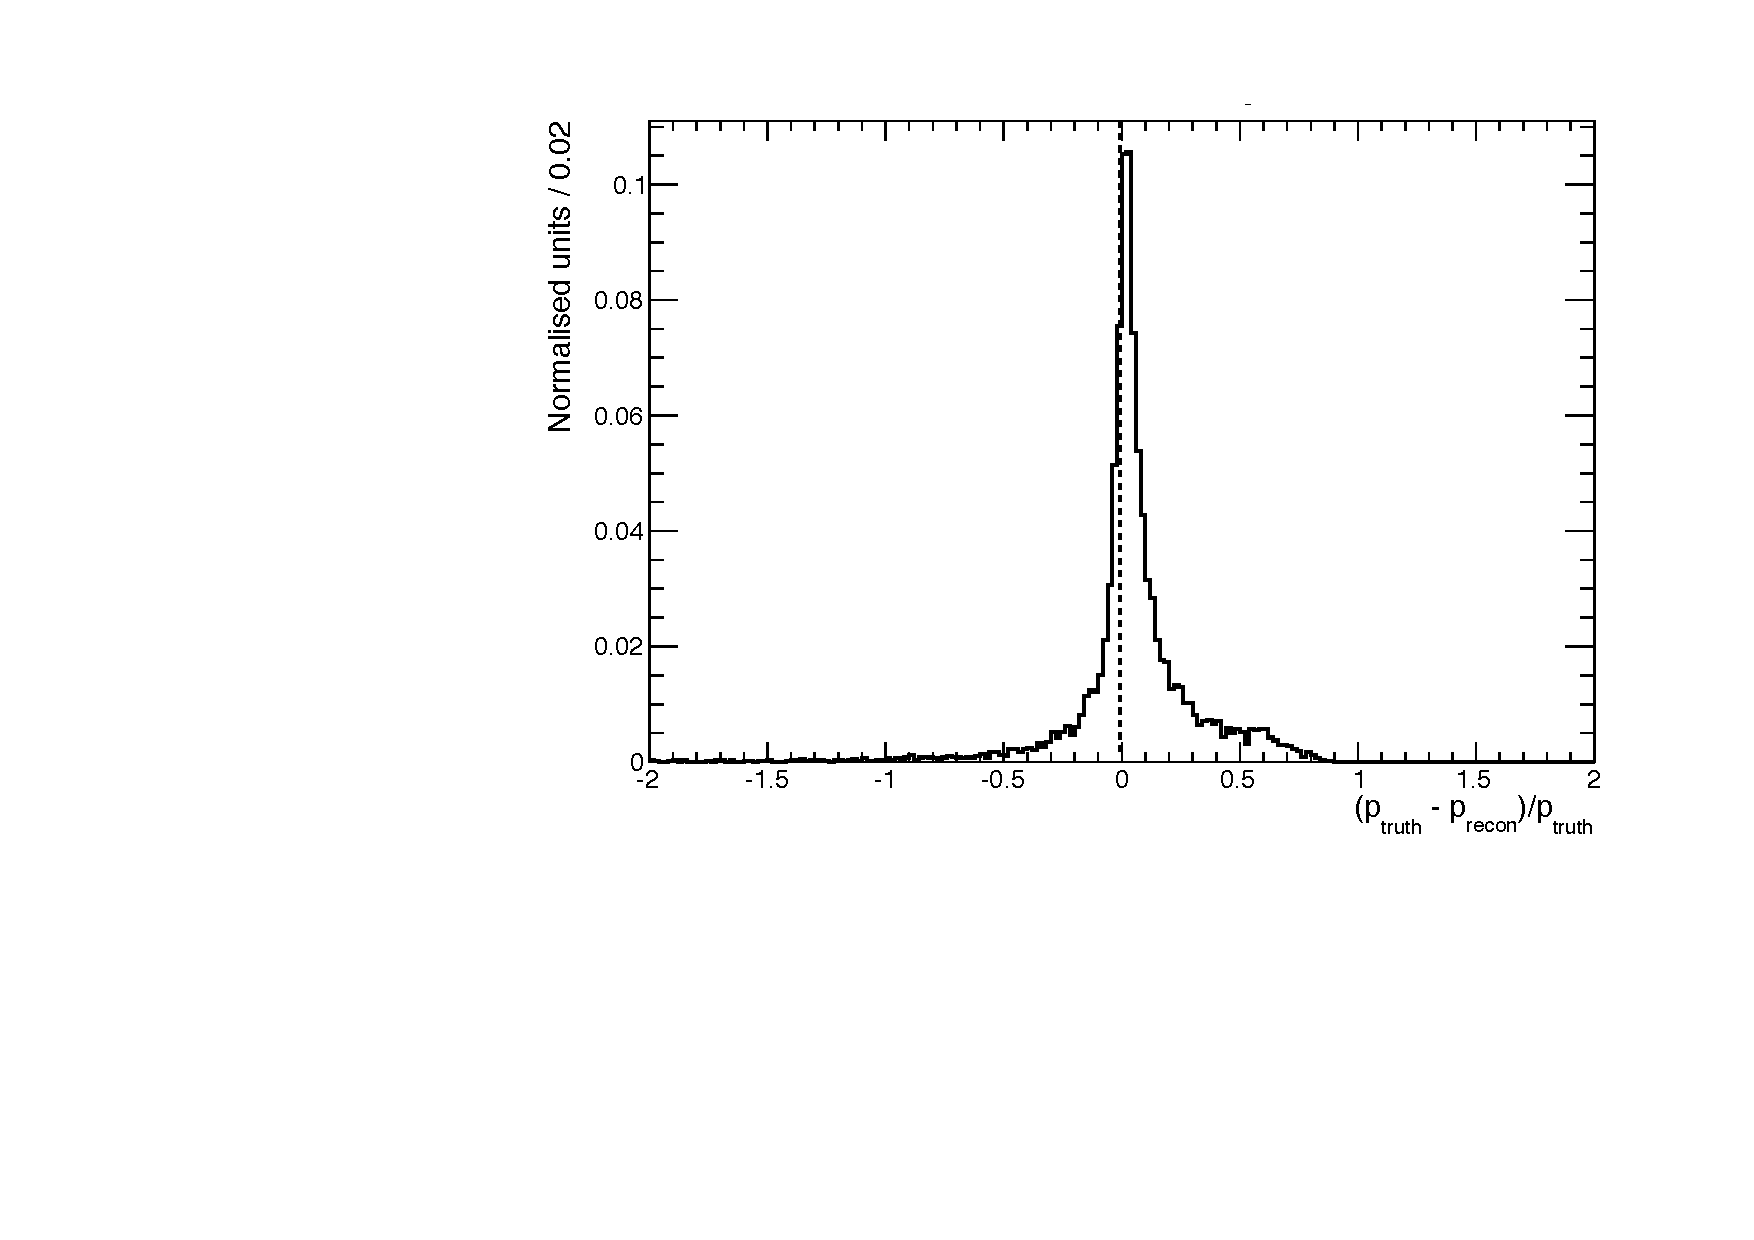
\includegraphics[width=100mm]{Chapter4/figures/recon_diff_ccqe.pdf}
%	\caption{The difference between reconstructed and truth momentum of muons within the TPC for CCQE interactions only. This is quantified by calculating $(p_{truth} - p_{recon})/p_{truth}$ for each CCQE neutrino interaction. The slight asymmetry in the plot of an excess of values $>$0 arises from the approximation that all the muons momentum is transverse.}
%	\label{fig:neutrinoCCQEMomReconDiff}
%\end{center}
%\end{figure}
%	
%\subsection{Momentum Reconstruction of Neutrinos in the TPC}
%The total neutrino momentum, $\boldsymbol{p}_{\nu}$, is given by the magnitude of the sum of the momentum of all outgoing particles, shown in equation \ref{eq:totalNuMom1} for $n$ particles originating from the neutrino interaction. 
%\begin{equation}
%	|\boldsymbol{p}_{\nu}| = |\boldsymbol{p_{a}} + \boldsymbol{p_{b}} + ... + \boldsymbol{p_{n}}| = |\sum^{n}_{i}{\boldsymbol{p}_{i}}|
%	\label{eq:totalNuMom1}
%\end{equation}
%Although neutrinos pertain mass, it is so small in comparison to the energies in the context of LAGUNA-LBNO that they can be considered as zero and the neutrino energy is simply proportional to its momentum, $E_{\nu} = p_{\nu}c$. Thus reconstruction of the neutrinos energy is determined from the reconstruction of each outgoing particles momentum, shown in equation \ref{eq:totalNuMom2}.
%\begin{equation}
%	E_{\nu} = |\boldsymbol{p}_{\nu}|c = c\sqrt{ \sum^{n}_{i}{\boldsymbol{p}_{i}\cdot\boldsymbol{p}_{i} } + 2 \Big[ \sum_{i \neq j}^{n} \sum_{j}^{n}\boldsymbol{p}_{i}\cdot\boldsymbol{p}_{j} \Big]}
%	\label{eq:totalNuMom2}
%\end{equation}
%The second term in equation \ref{eq:totalNuMom2} can be determined by measurement of the angle between each track, however such a measurement or reconstruction is not performed within this study. Only measurement of the transverse momentum of charged particles is performed within the TPC, and as a result it is better to use conservation of energy:
%\begin{equation}
%	E_{\nu} = \sum^{n}_{i}E_{i} = \sum^{n}_{i}\sqrt{\boldsymbol{p}_{i}\cdot\boldsymbol{p}_{i} + m^{2}_{i}}
%	\label{eq:totalNuEnergy1}
%\end{equation}
%Particle identification is not performed within this study and the focus is to understand how well the neutrinos energy can be reconstructed from momentum measurements in the TPC alone. Two approximations are made to equation \ref{eq:totalNuEnergy1} to simplify the problem: $\boldsymbol{p}_{i}\cdot\boldsymbol{p}_{i}$ $\sim$ $p^{2}_{trans}$ and $p^{2}_{i}$ $\gg$ $m_{i}^{2}$.  This is a certainly reasonable approximation for muons as they are highly energetic and very forward going but far less accurate for protons and pions. 
%
%The reconstructed neutrino energy is then simply proportional to the sum of the transverse momentum of each particle showing in the TPC:
%\begin{equation}
%	E_{\nu} \approx c\sum^{n}_{i}{p^{trans}_{i}}
%	\label{eq:totalNuMom3}
%\end{equation}
%
%Only charged particles contribute to the total reconstructed neutrino momentum and as a result momentum of neutral particles, mainly photons and neutrons, cannot be measured within the TPC. For NC interactions this is especially important and the TAS will provide instrumental in measurement of their energies. Figure \ref{fig:neutrinoMomReconVsTruth} shows the reconstructed neutrino momentum as a function of truth neutrino momentum binned on an event-by-event basis for all neutrino interaction types. It is noticeable from this figure that momentum reconstruction of the neutrino using this technique is quite poor mainly due to the neutral particle contribution of outgoing particles. This is more apparent in figure \ref{fig:neutrinoMomReconDiff} which again shows the difference in reconstructed and truth momentum of the neutrino, $(p_{truth} - p_{recon})/p_{truth}$. The asymmetry is much larger here than compared to the same figure for CCQE only, due heavily to NC interactions, with neutrinos, neutrons and photons taking away energy from the vertex that cannot be measured with the TPC. It is however centred on zero indicating that for a large amount of events reconstruction of the neutrino energy can be done well with the TPC alone.
%
%\begin{figure}[htbp]
%\begin{center}
% 	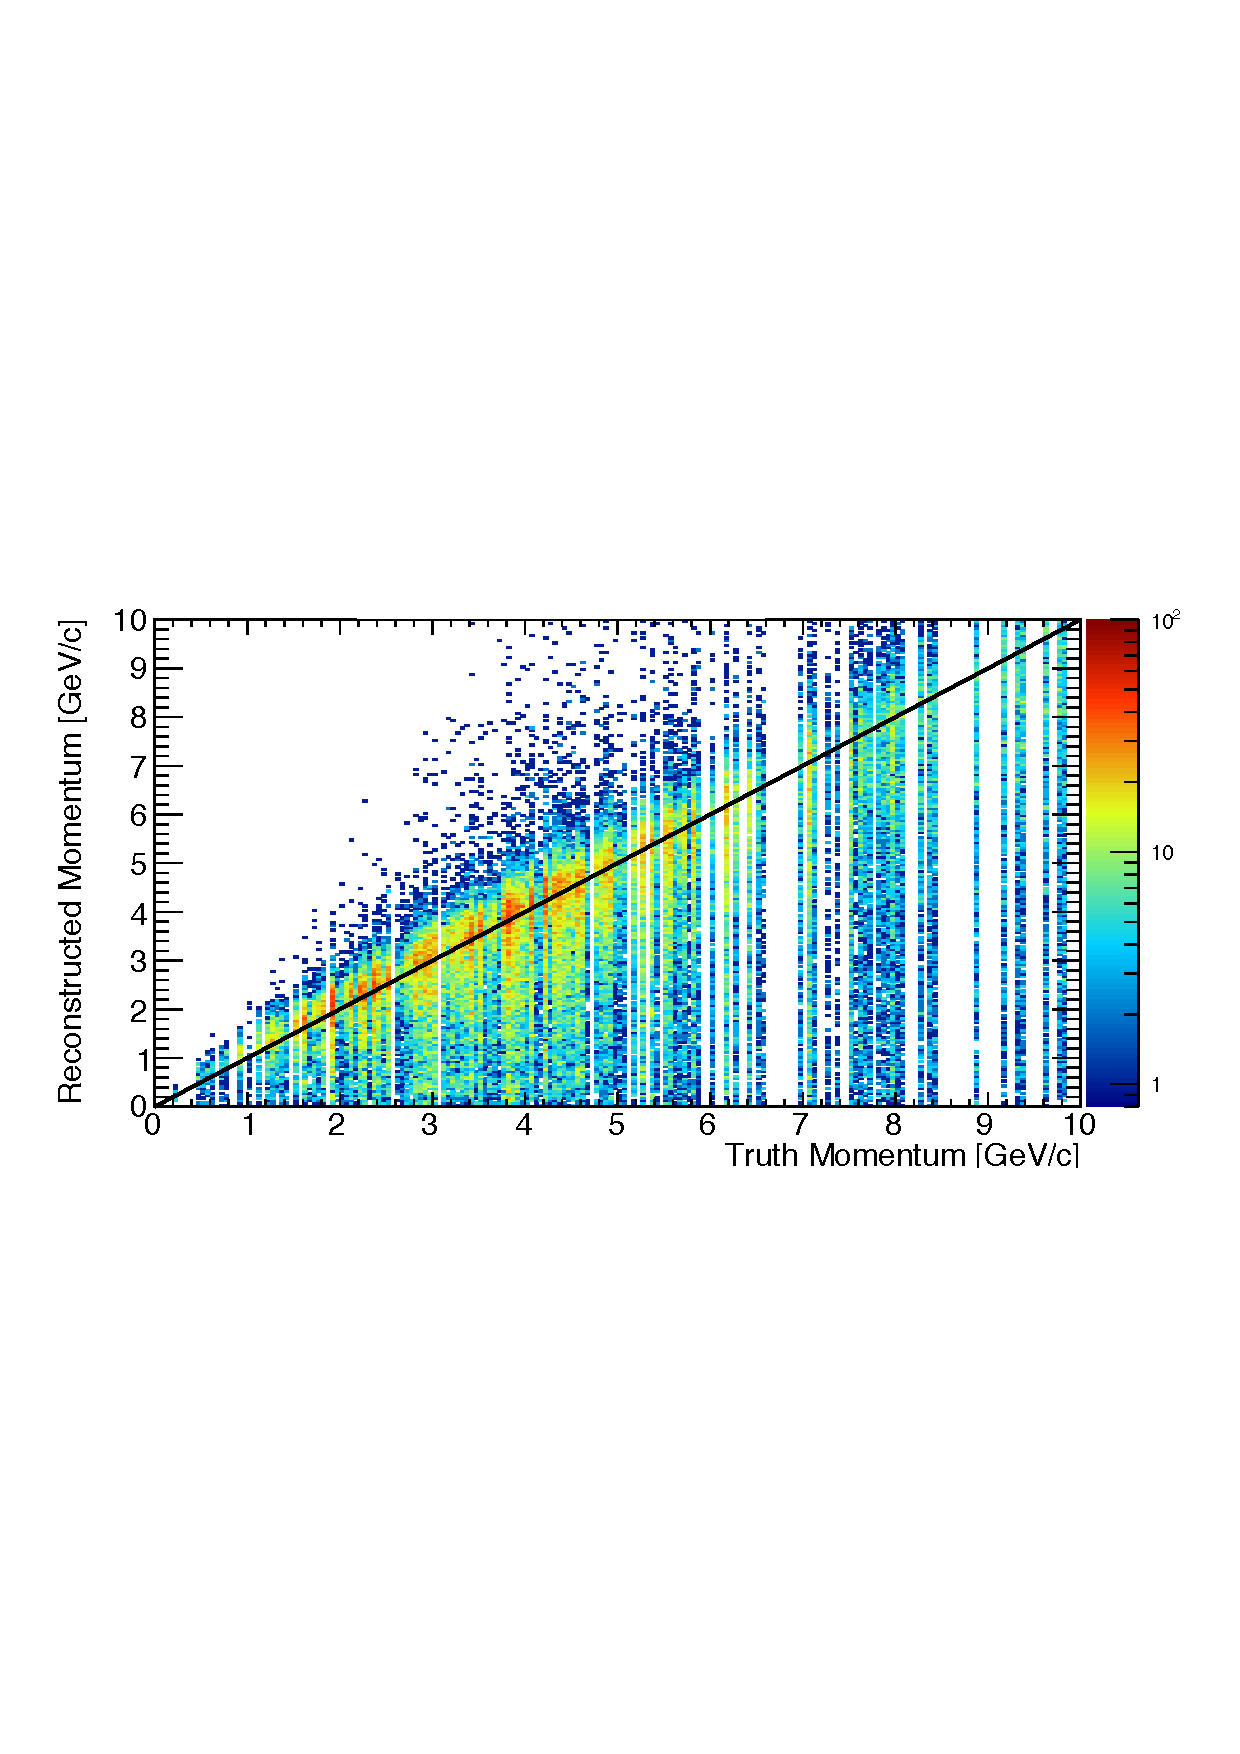
\includegraphics[width=74mm,height=48mm]{Chapter4/figures/recon_truth_neutrino_h2d.pdf}
% 	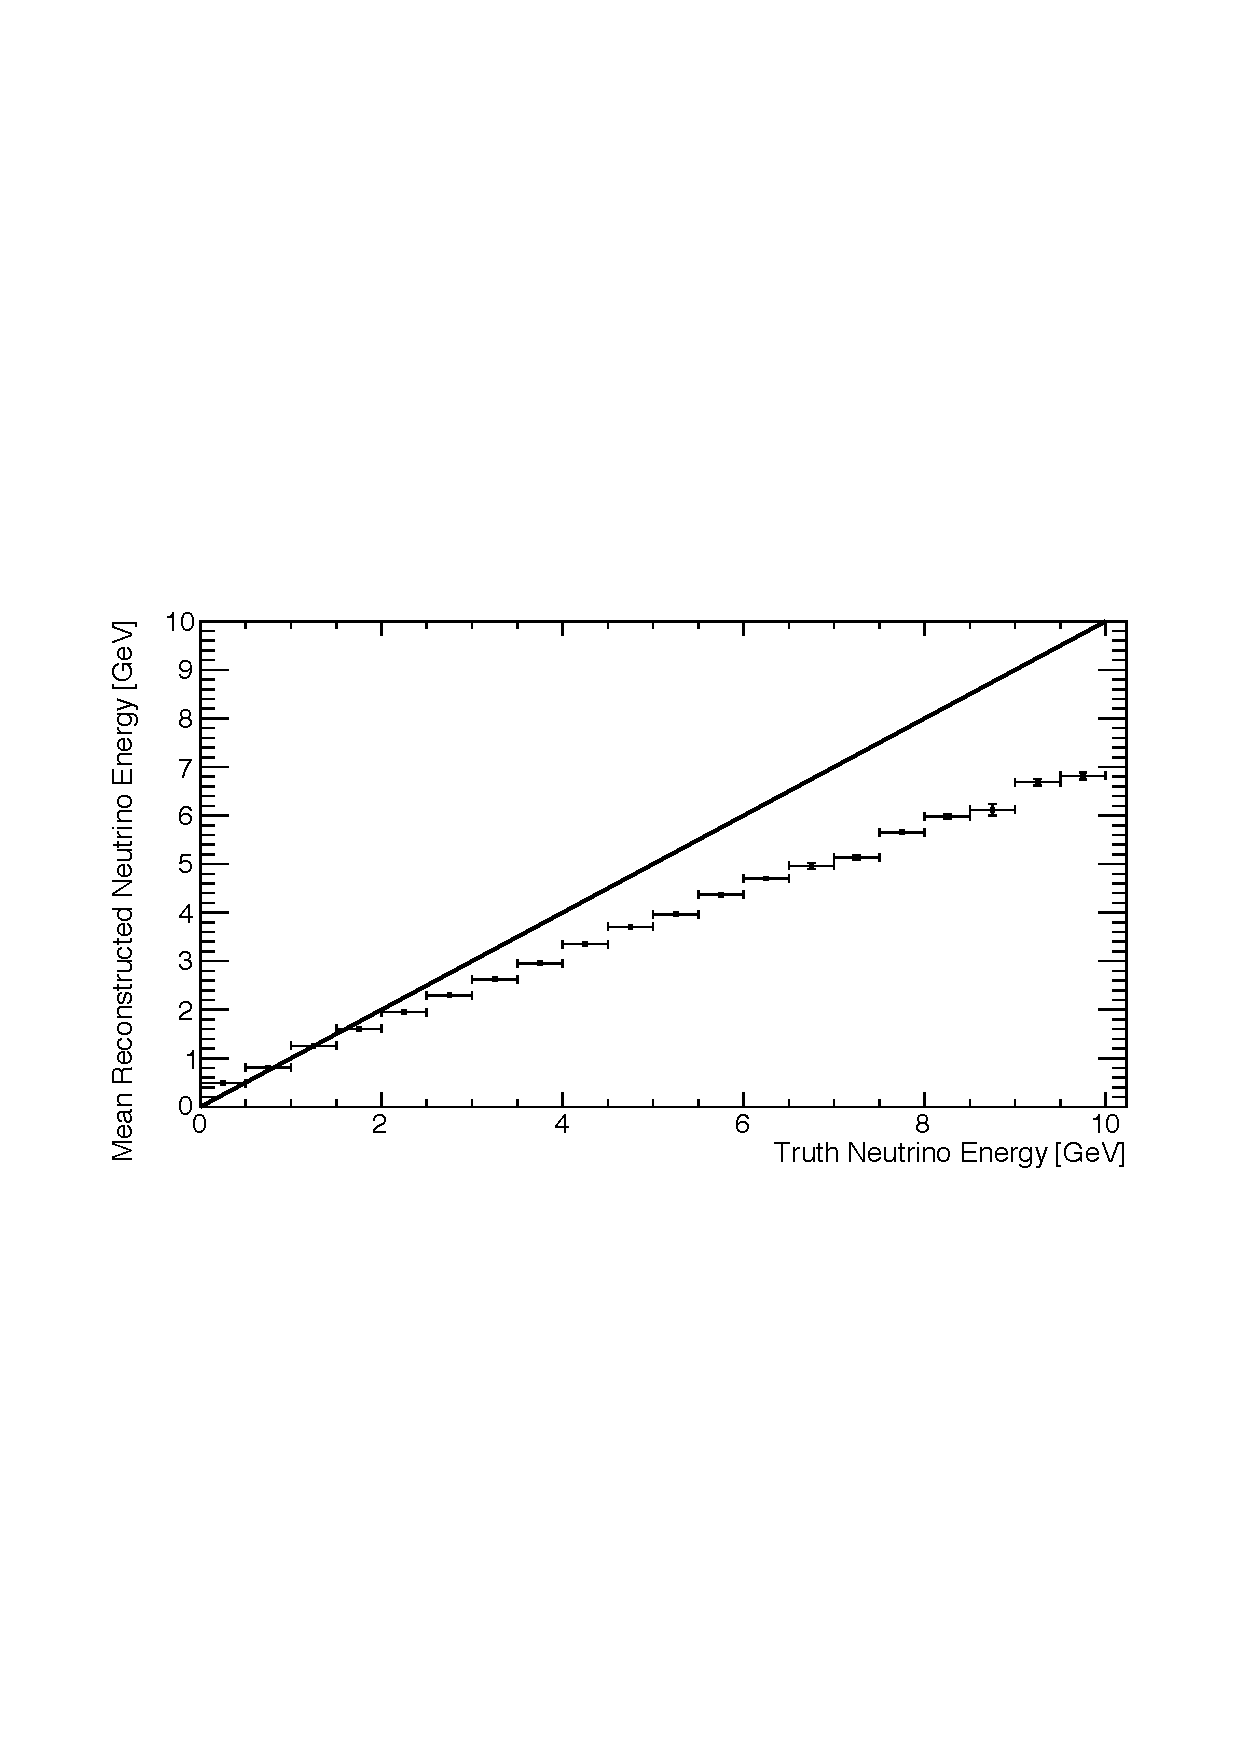
\includegraphics[width=74mm,height=48mm]{Chapter4/figures/mean_recon_neutrino_energy_all.pdf}
%	\caption{Left: The reconstructed neutrino momentum as a function of the truth neutrino momentum for all (CC + NC) interaction types. Right: The mean reconstructed neutrino energy as a function of truth neutrino energy. The mean reconstructed value is determined from all events that fall within each 0.5 GeV truth bin. Error bars indicate the standard deviation value of the mean, 1$\sigma$. Results based on simulation of exposure 9.6 $\times$ 10$^{19}$ p.o.t. }
%	\label{fig:neutrinoMomReconVsTruth}
%\end{center}
%\end{figure}
%
%\begin{figure}[htbp]
%\begin{center}
% 	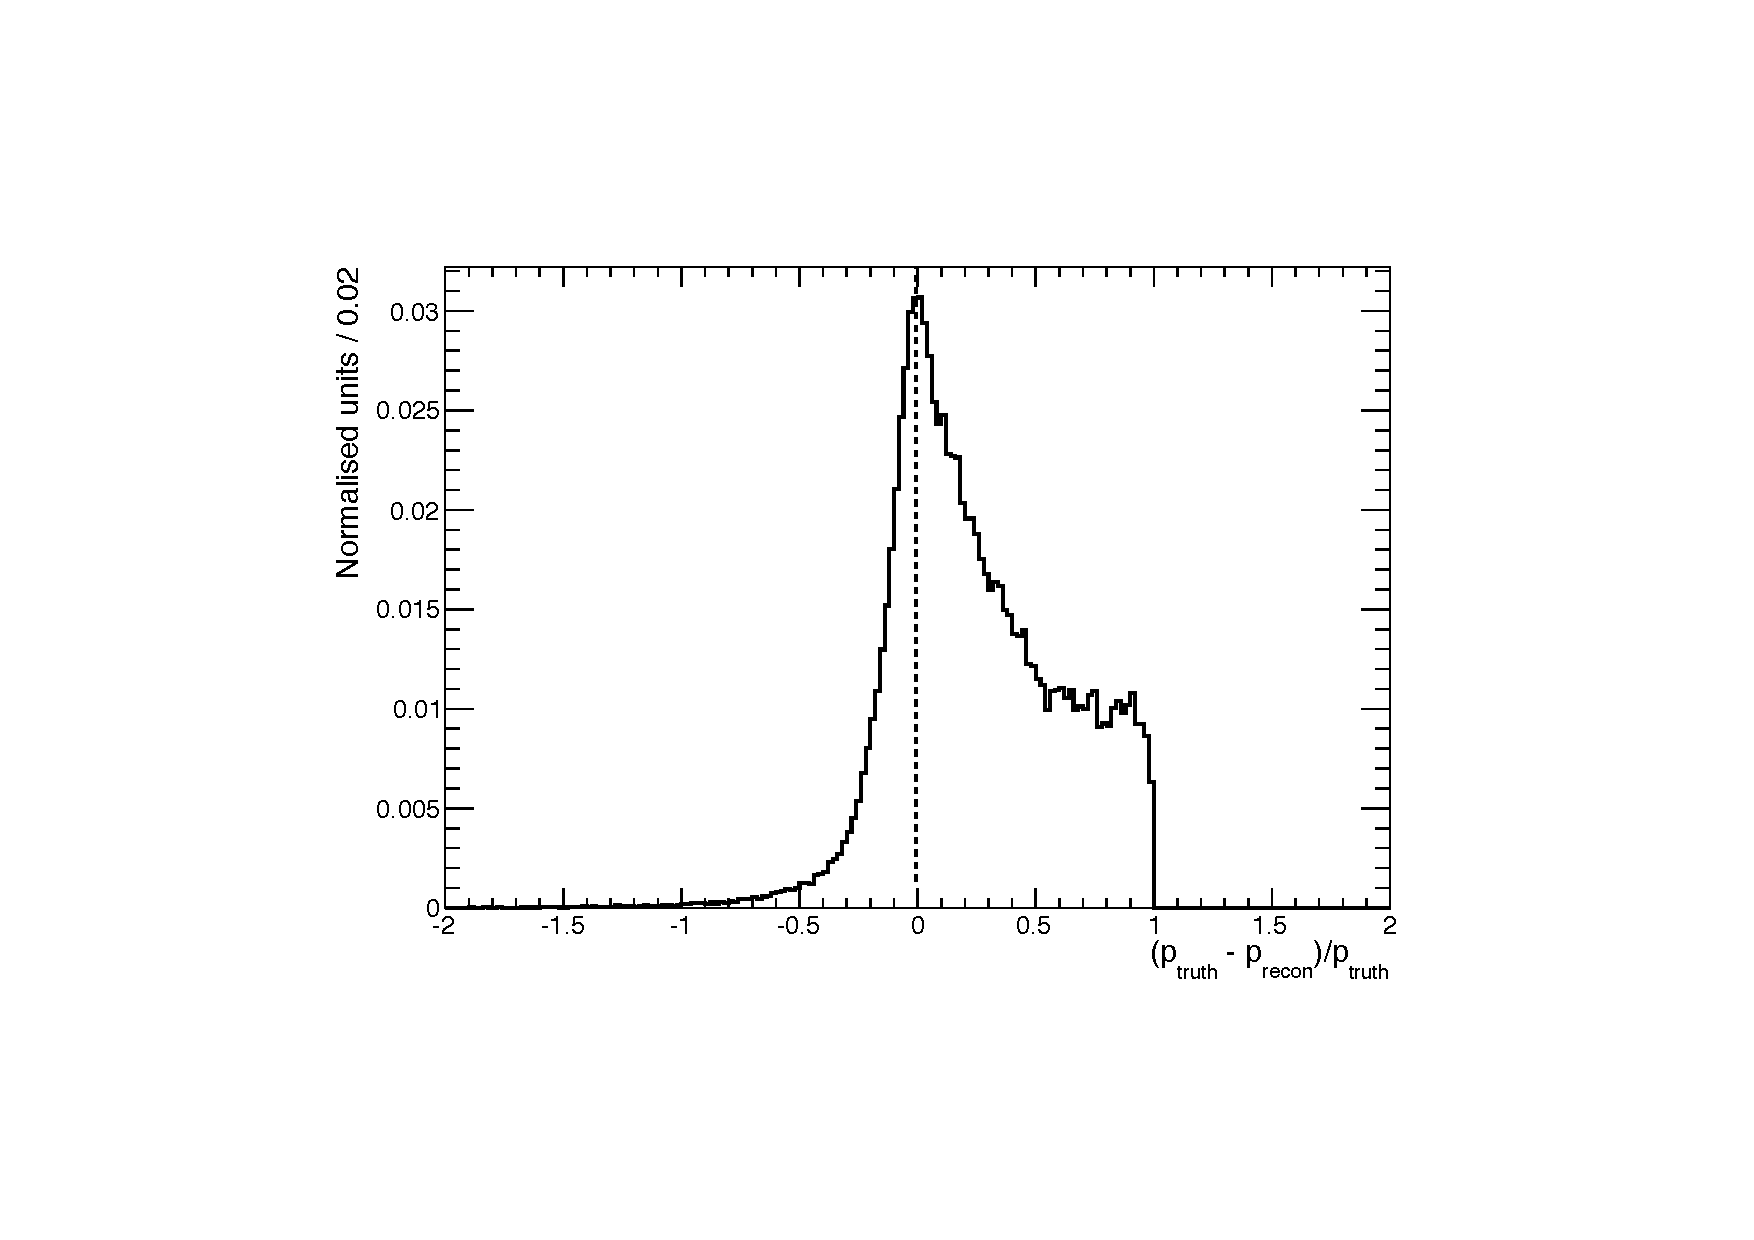
\includegraphics[width=76mm]{Chapter4/figures/recon_diff_all.pdf}
%	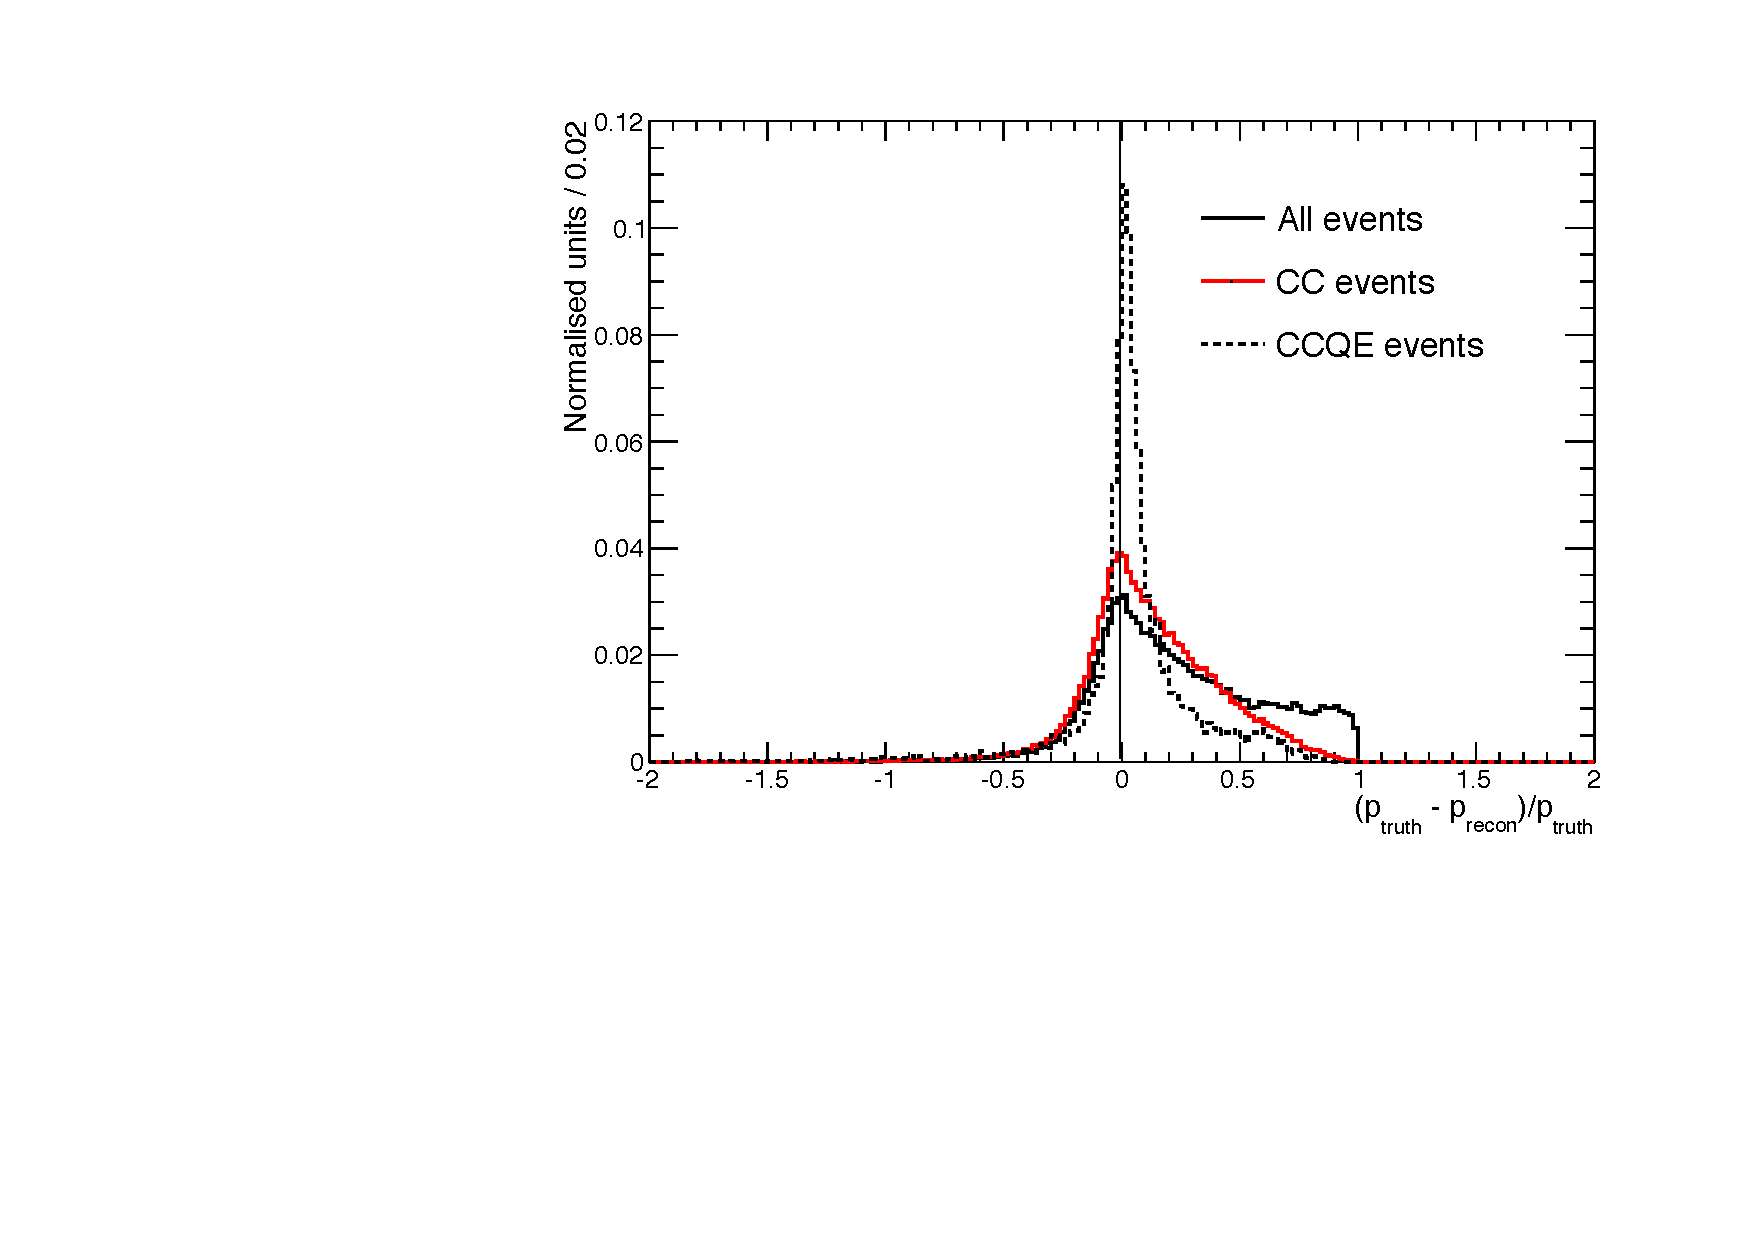
\includegraphics[width=76mm]{Chapter4/figures/recon_diff_comparision.pdf}
%	\caption{Left: The difference between reconstructed and truth momentum of muons within the TPC for all neutrino interaction types. This is quantified by calculating $(p_{truth} - p_{recon})/p_{truth}$ for each neutrino interaction. Right: The same plot compared with event selections of CC and CCQE only. Results based on simulation of exposure 9.6 $\times$ 10$^{19}$ p.o.t but normalised to number of events.}
%	\label{fig:neutrinoMomReconDiff}
%\end{center}
%\end{figure}
%
%Comparison of the neutrino truth and reconstructed energies, for all events and CCQE only events, is shown in figure \ref{fig:neutrinoEnergyRecon}. Although CCQE interactions are well reconstructed with the TPC, they occur at much lower energies and hence shows a lower reconstructed neutrino energy spectrum than the truth. In order to gain an accurate description of the incident neutrino flux, DIS and RES events must be well reconstructed. Inclusion of these event types for reconstruction is however worse due to the large energy losses through neutral particles leaving the TPC.
%
%\begin{figure}[htbp]
%\begin{center}
% 	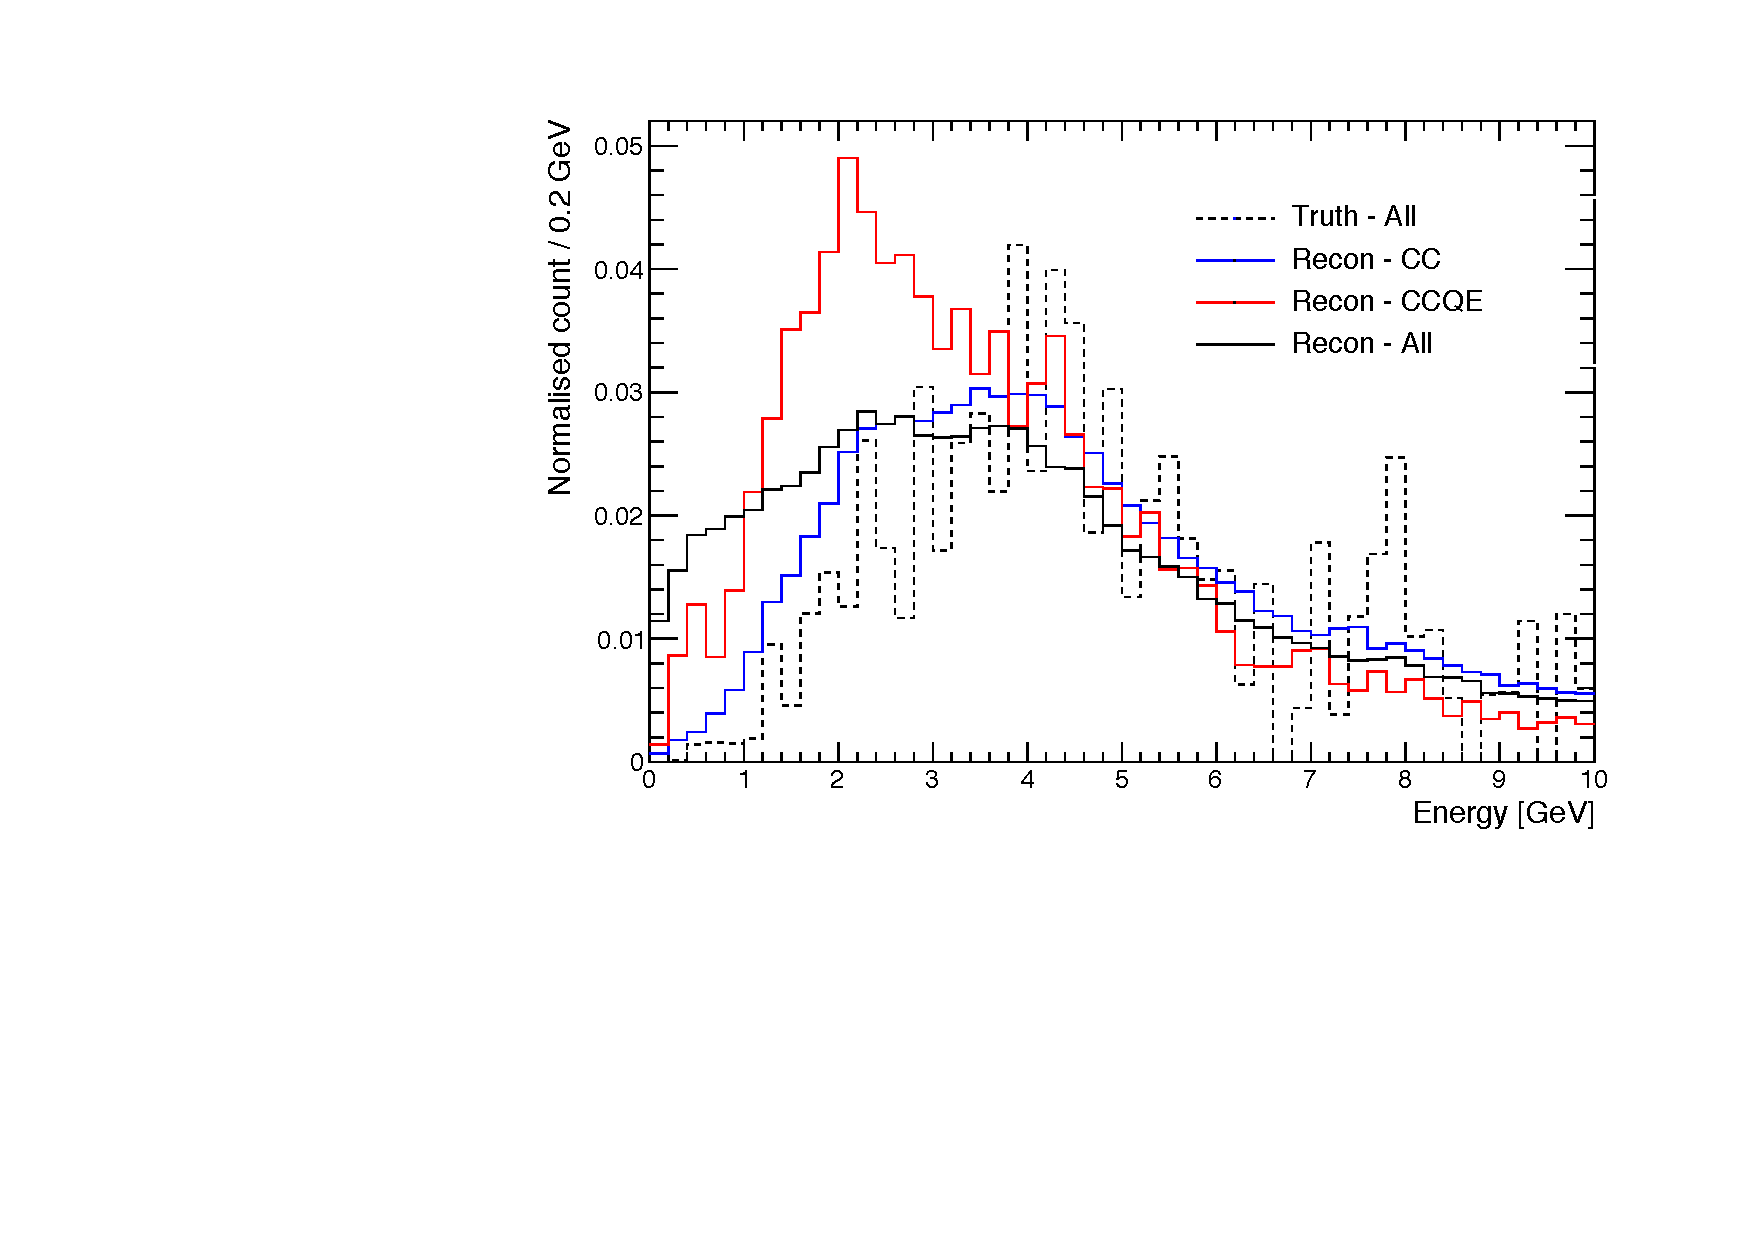
\includegraphics[width=140mm]{Chapter4/figures/neutrino_reconEnergy_h1d_comparision.pdf}
%	\caption{The reconstructed neutrino energy is shown for all event types simulated (solid black line) and CCQE only (solid red line) against the truth neutrino energy in the 0 - 10 GeV regime. Histograms for truth and all event reconstruction are normalised to the total number of events generated whereas CCQE reconstructed events are normalised to the number CCQE events only.}
%	\label{fig:neutrinoEnergyRecon}
%\end{center}
%\end{figure}
%
%%The total transverse momentum of all visible (charged) tracks in the TPC is then simply the sum of each reconstructed transverse momentum, given by equation \ref{eq:totalTransMom}.
%%\begin{equation}
%%	p_{TOT}^{trans} = \sum^{tracks}_{i}{p_{i}^{trans}}
%%	\label{eq:totalTransMom}
%%\end{equation}
%
%\subsection{Particle Energy Loss in the TPC}
%Particle identification is not incorporated into the reconstruction process but future studies should examine the potential of particle identification within the TPC. Determination of how particles lose energy in the TPC, precisely $dE/dx$, can be a powerful technique to identify different particle types. Taking the total energy deposited by each charged track, $\Delta E$, and the range of the track in the TPC, $\Delta x$, $dE/dx$ = $\Delta E/\Delta x$. Upon dividing by the density of the TPC gas, $\rho$ = 0.035gcm$^{-3}$, then scales to units of MeV cm$^{2}$ g$^{-1}$.
%\begin{figure}[htbp]
%\begin{center}
% 	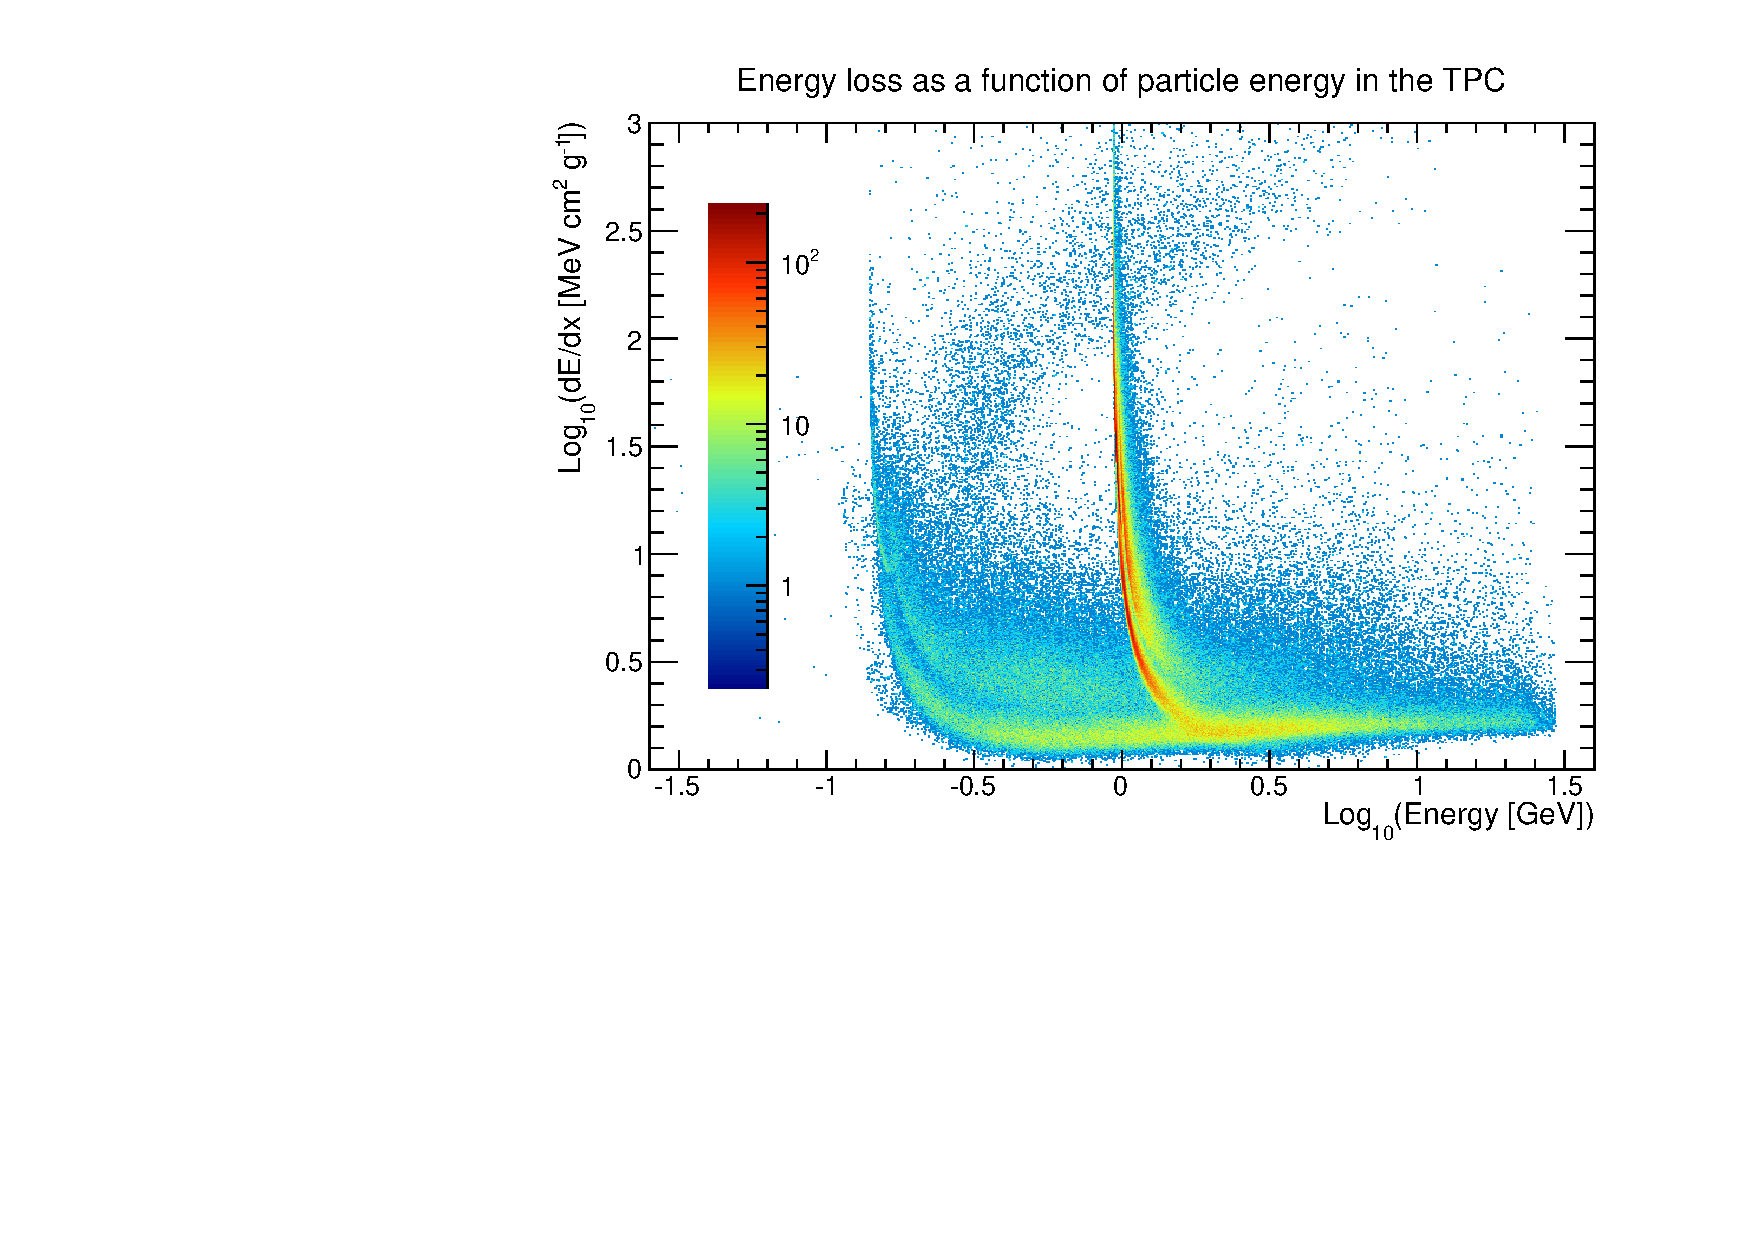
\includegraphics[width=120mm]{Chapter4/figures/dEdx_tpc_all.pdf}\\
% 	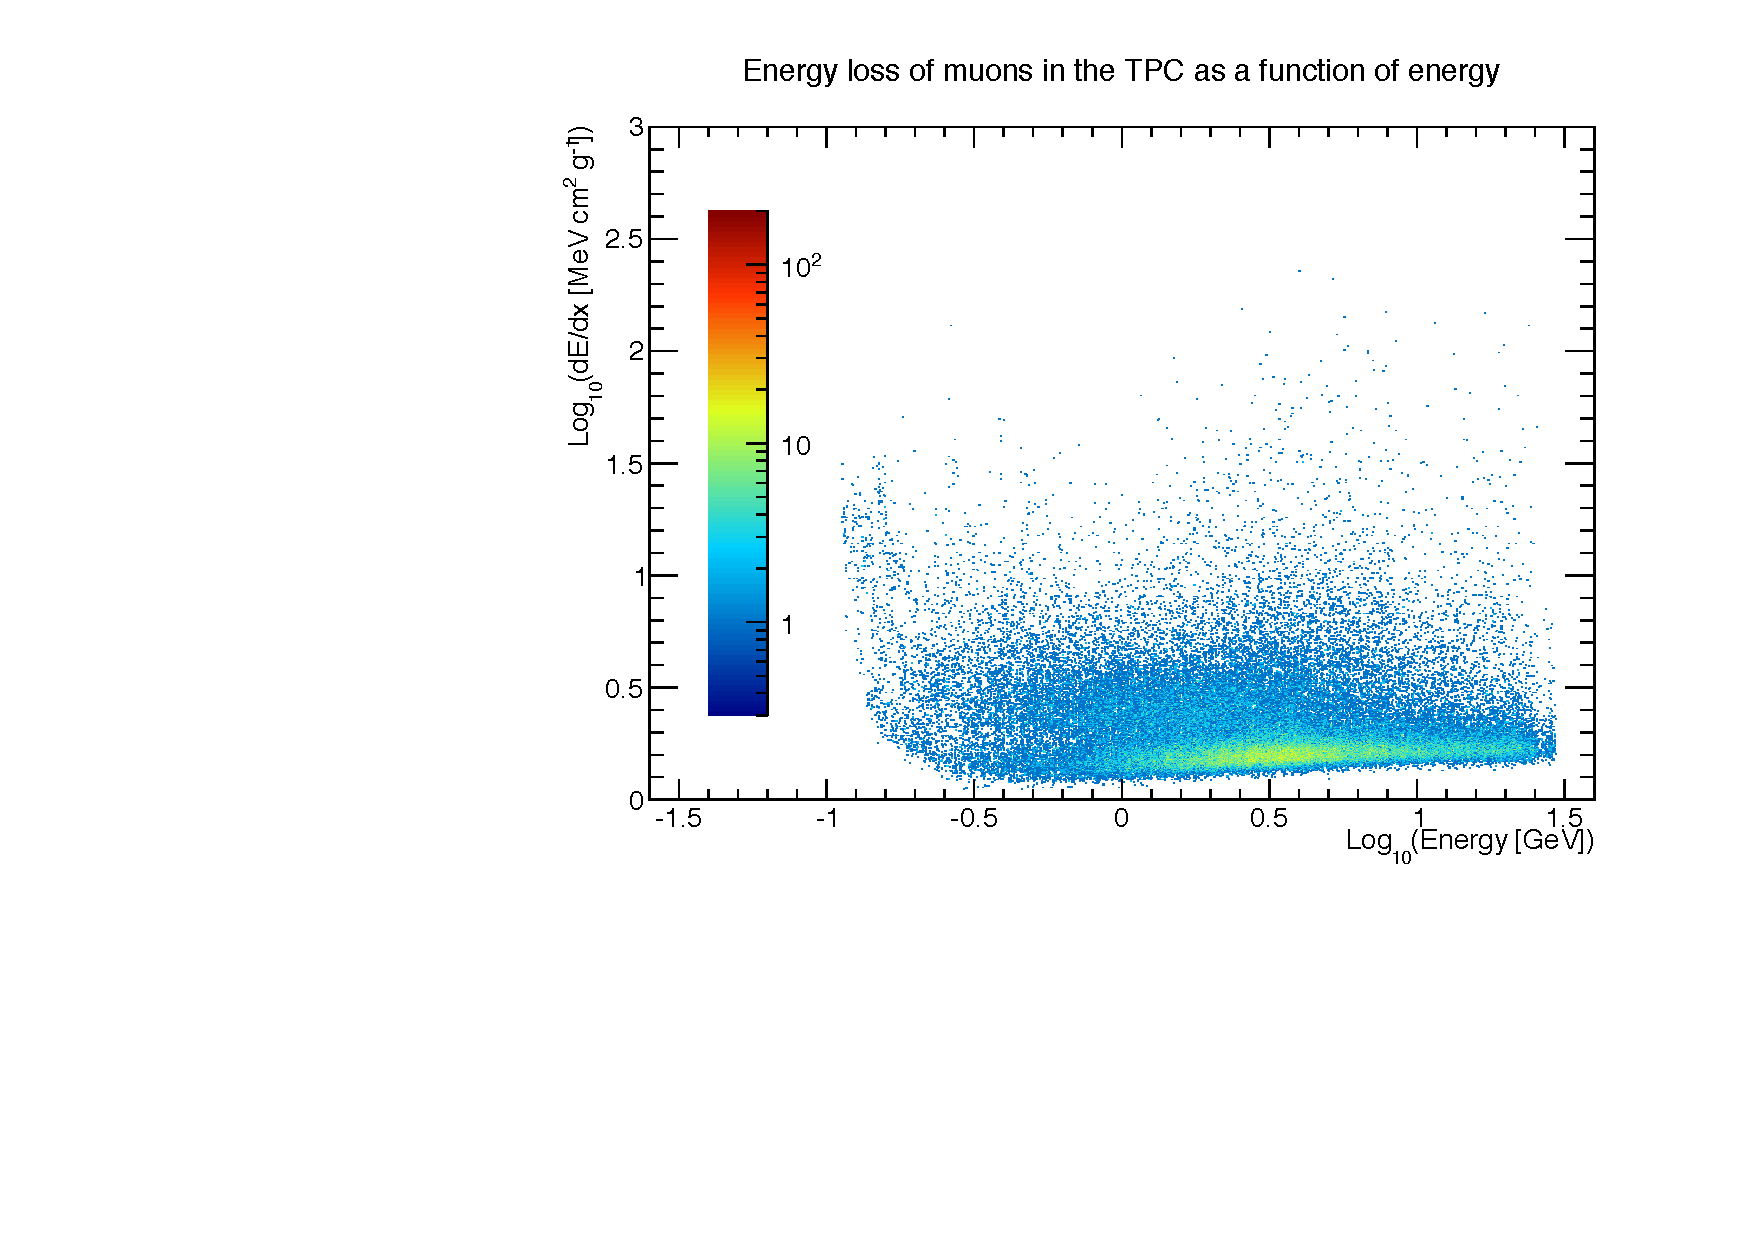
\includegraphics[width=50mm]{Chapter4/figures/dEdx_tpc_muon.pdf}
% 	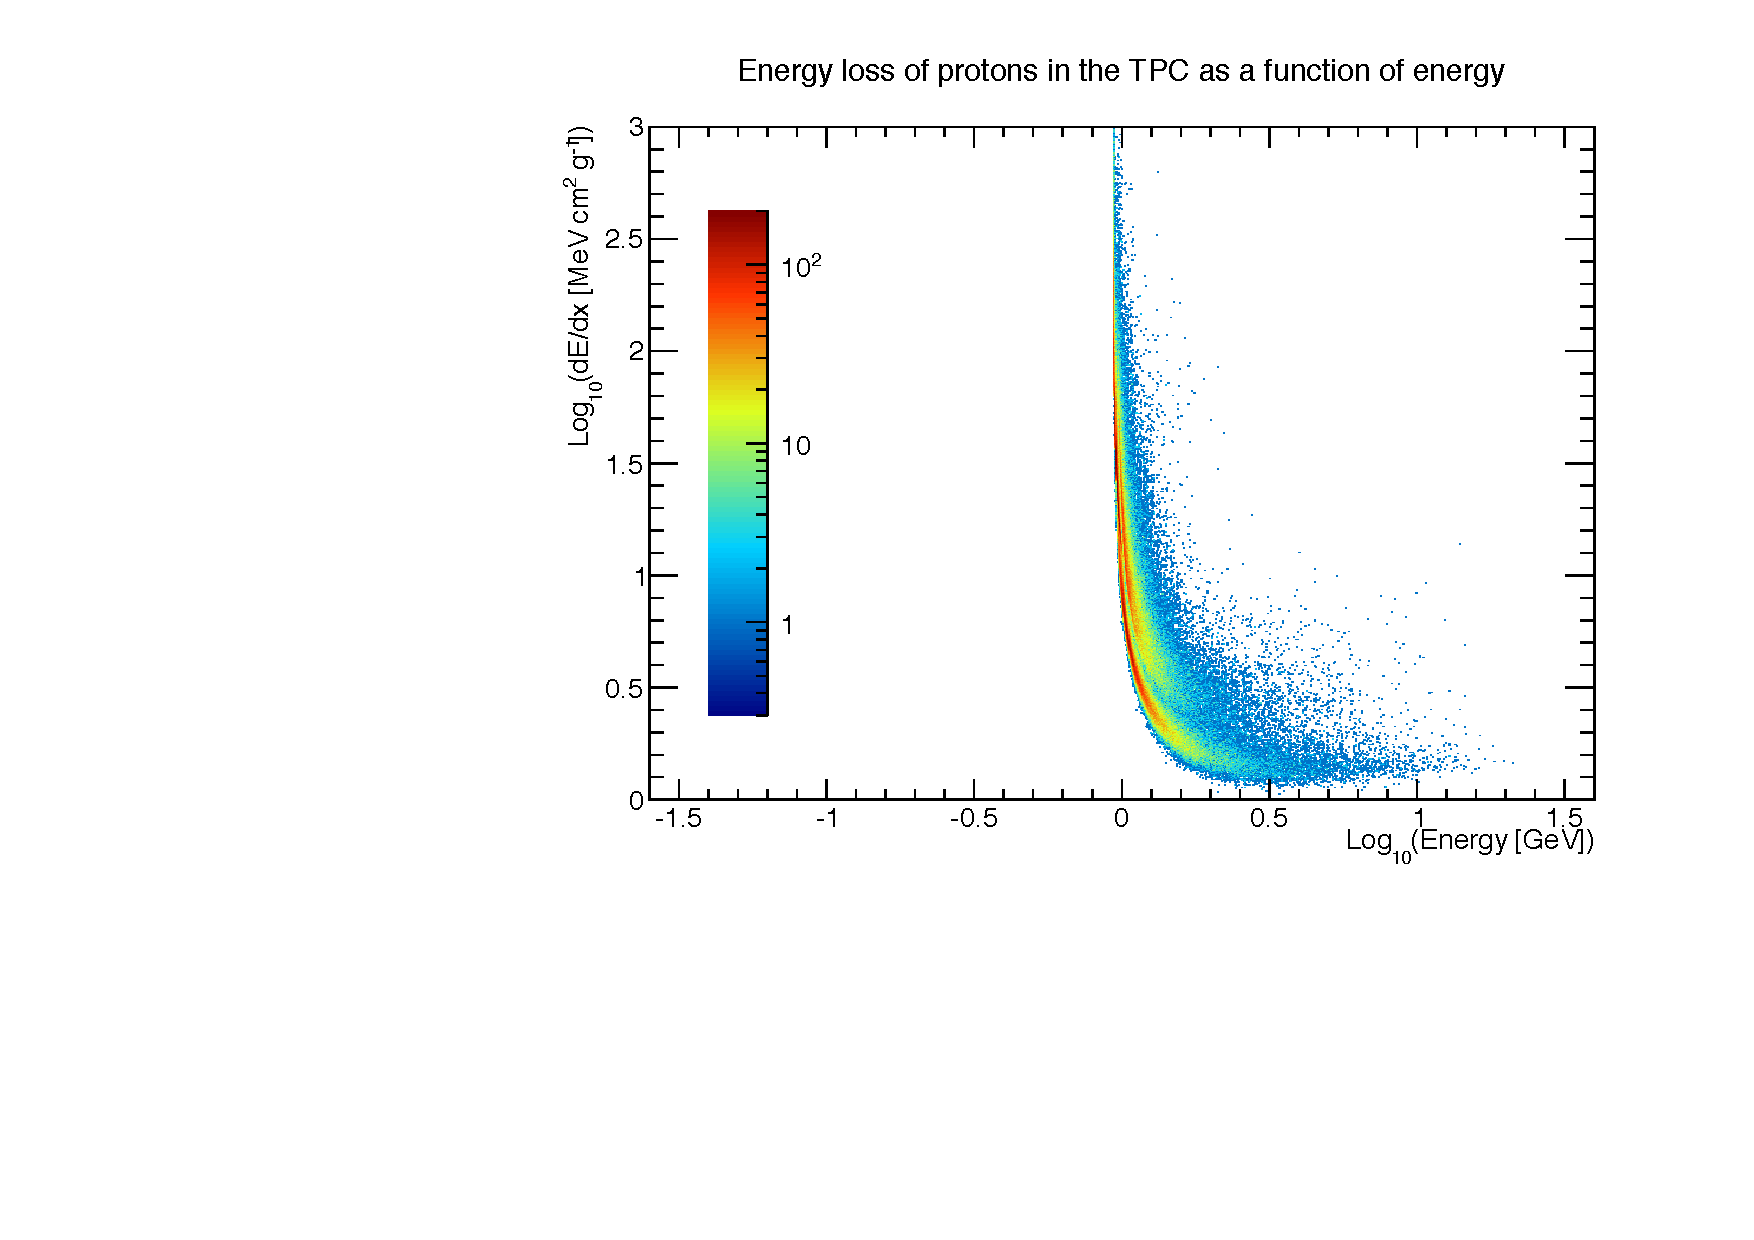
\includegraphics[width=50mm]{Chapter4/figures/dEdx_tpc_proton.pdf}
% 	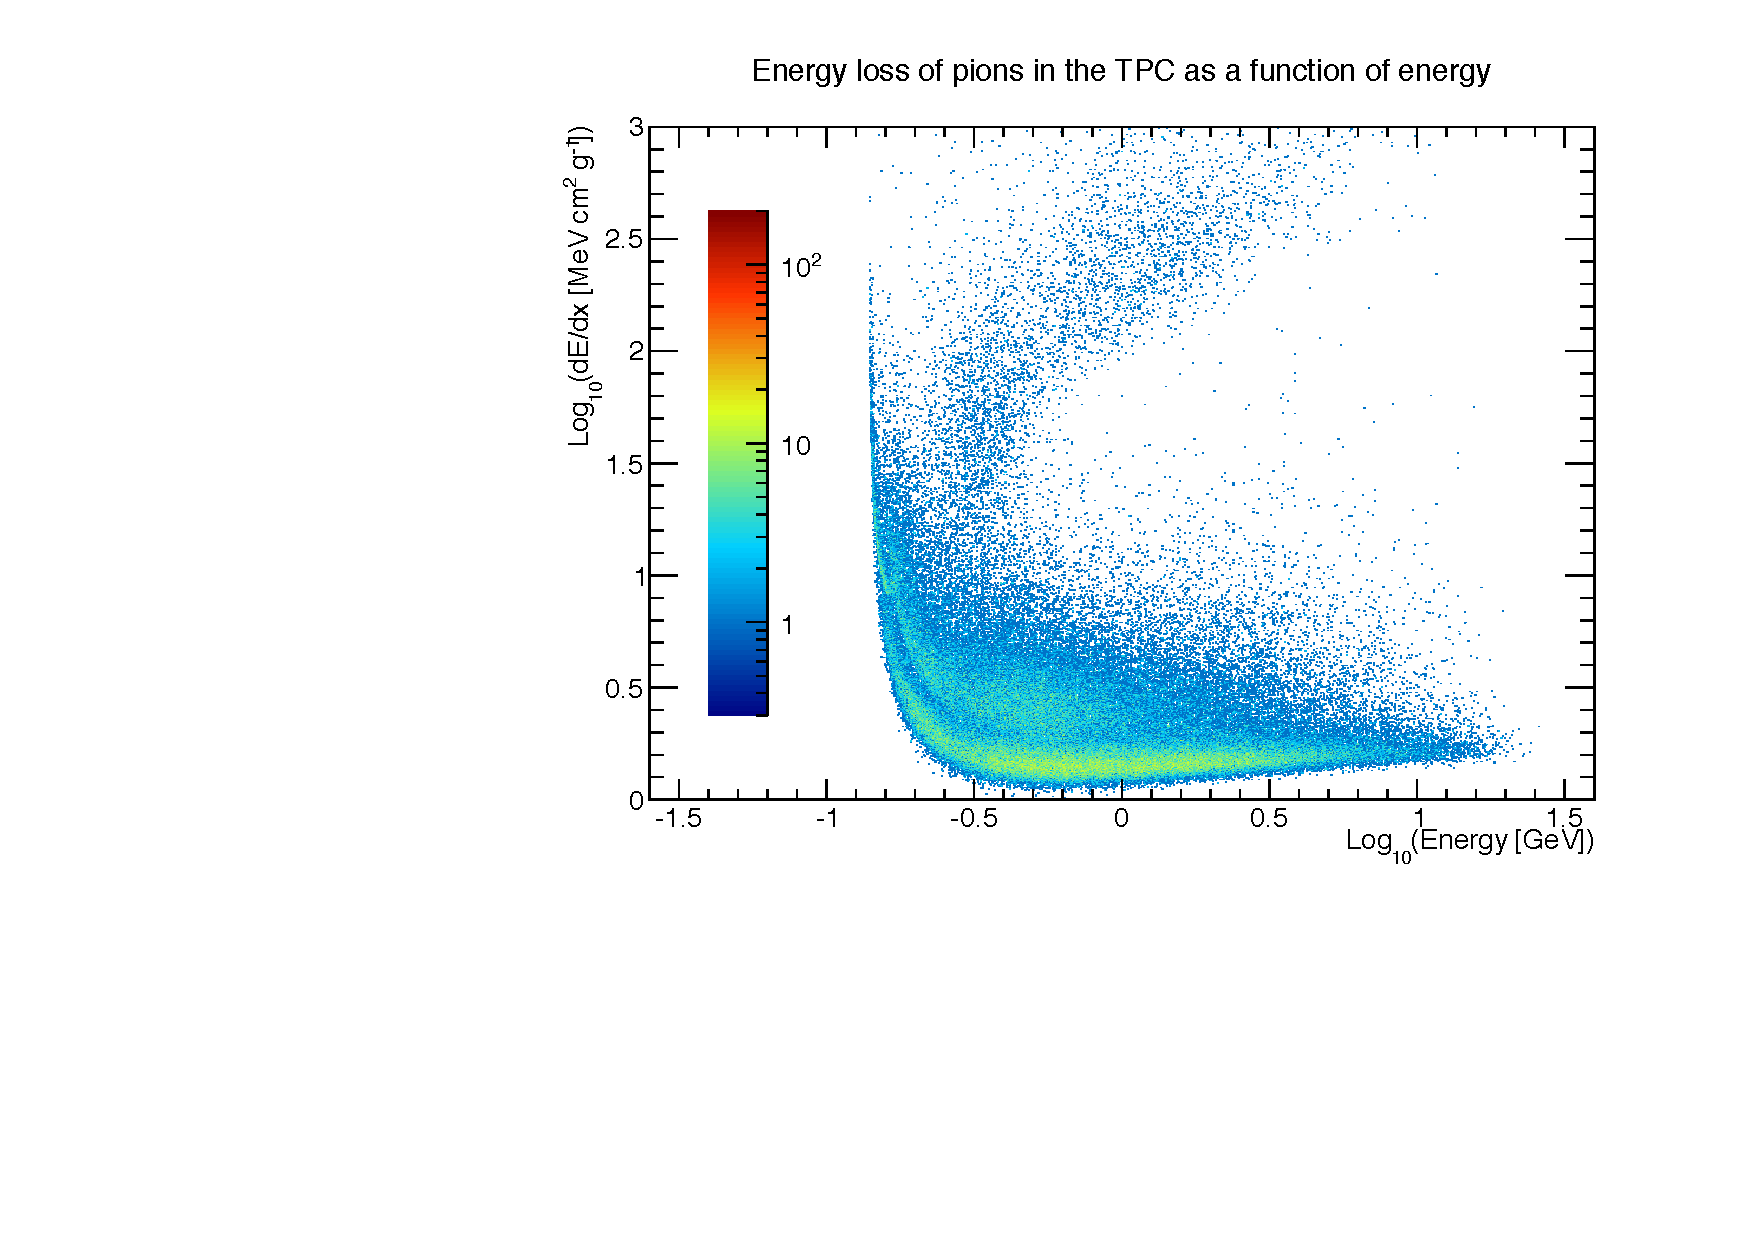
\includegraphics[width=50mm]{Chapter4/figures/dEdx_tpc_pion.pdf}
%	\caption{The energy loss of charged particles within the TPC as determined by dE/dx as a function of truth energy. Muons, protons and pions are collectively shown on the large plot, while they are shown individually from left to right respectively on the smaller plots.}
%	\label{fig:energyLossTPCrecon}
%\end{center}
%\end{figure}
%
%Discrimination between muons and pions using this technique is difficult for energies above $\sim$0.5 GeV. With the majority of muons having energies larger than this other techniques will need to be employed. Identifying protons can be done for particles with energies below $\sim$1.5 GeV.
%
\section{Energy Reconstruction of $\pi^{0}$s in the TAS}
At this point we have not directly focussed on the ND performance and its reconstruction capabilities, we next examine a selected demonstration of the ND performance focusing on energy reconstruction of $\pi^{0}$s using the TAS. It is clear from the previous sections that this is not only important to detect $\pi^{0}$s but to also reconstruct their energy as photons originating from their decay can carry away a considerable amount of energy in both CC and NC neutrino interactions, as shown in figure \ref{fig:CCandNCKinEnergyRatios}. To reconstruct a $\pi^{0}$ involves the reconstruction of the two photons that led to its decay requiring good knowledge of the photon momentum to give an accurate measurement of the $\pi^{0}$ energy and to locate the neutrino interaction vertex. Particularly the latter is useful in NC interactions where no charged particles can be observed in the TPC.

Inclusion of the TAS aims to complement the TPC by measuring the energy deposited by photons. Almost all photons ($\sim$99\%) leaving the TPC arise from $\pi^{0}$ decays via: $\pi^{0} \rightarrow \gamma \gamma$. It was shown earlier that also they contribute to 30.7\% of the total number of particles leaving the TPC, with neutrons the second majority at 22.5\%. This equates to 0.5255 $\pm$ 0.0008 (stat) photons ppp. If the momentum of the outgoing photons can be determined it is then possible to reconstruct the original energy of the $\pi^{0}$, of which contribute to 12\% of all particles produced at the neutrino vertex (400 GeV PF beam). It is therefore strongly motivated to discuss potential reconstruction techniques for $\pi^{0}$s using the TAS sub detector. Although neutrons contribute heavily to the number of particles leaving the TPC they are not considered in this study, as they require different methods and techniques for reconstruction. 

The true kinetic energy spectrum of $\pi^{0}$s from neutrino interactions in the TPC can be seen in the right of figure \ref{fig:pi0KineticEnergy} with their multiplicities on the left. High multiplicities of up to 8 $\pi^{0}$s per neutrino interaction can occur, although such occurrences are rare. The average multiplicity is $\sim$1.2 per neutrino interaction in the TPC, with the majority of energies of $<$5 GeV. To understand how these can be reconstructed it is first necessary to understand how photons can be reconstructed within the TAS.

\begin{figure}[htbp]
\begin{center}
  	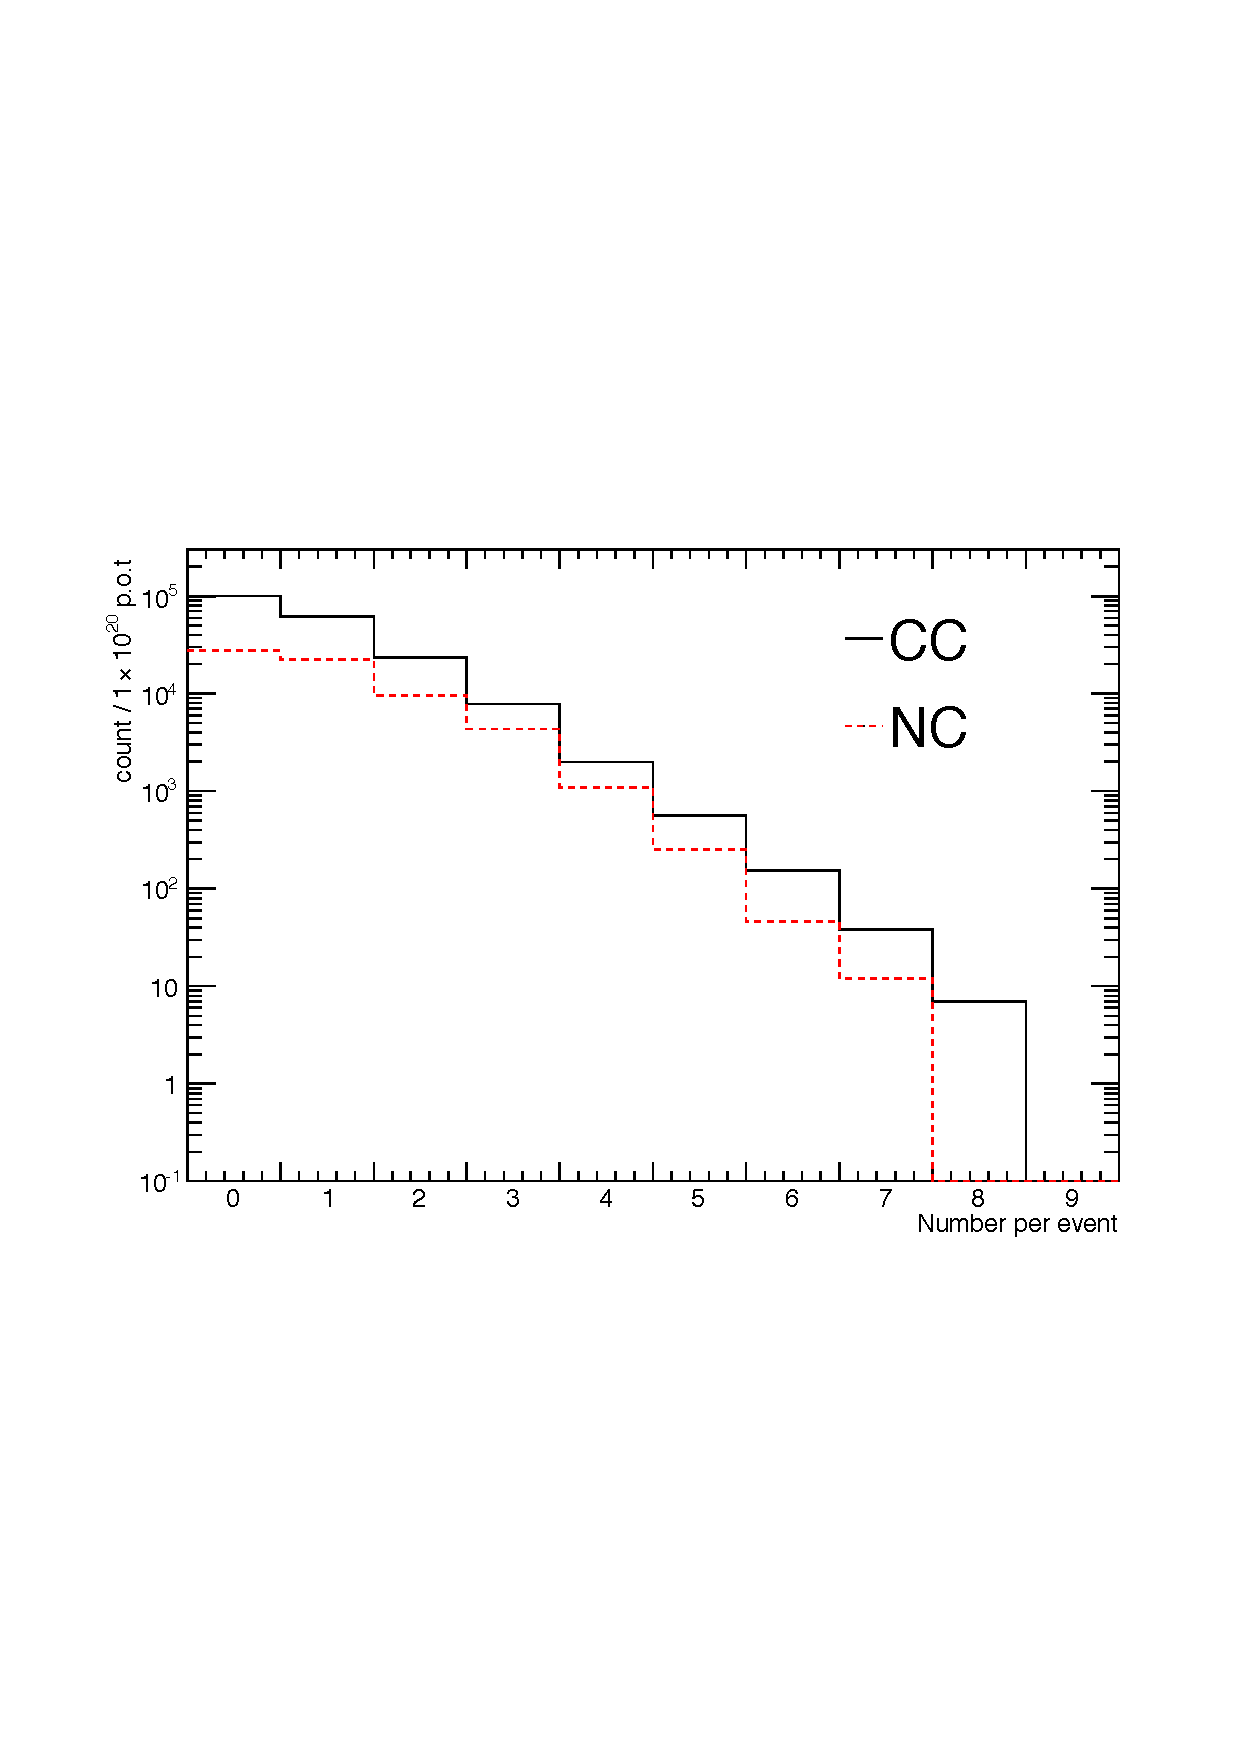
\includegraphics[width=76mm]{Chapter4/figures/piZeroMultiplicities.pdf}
  	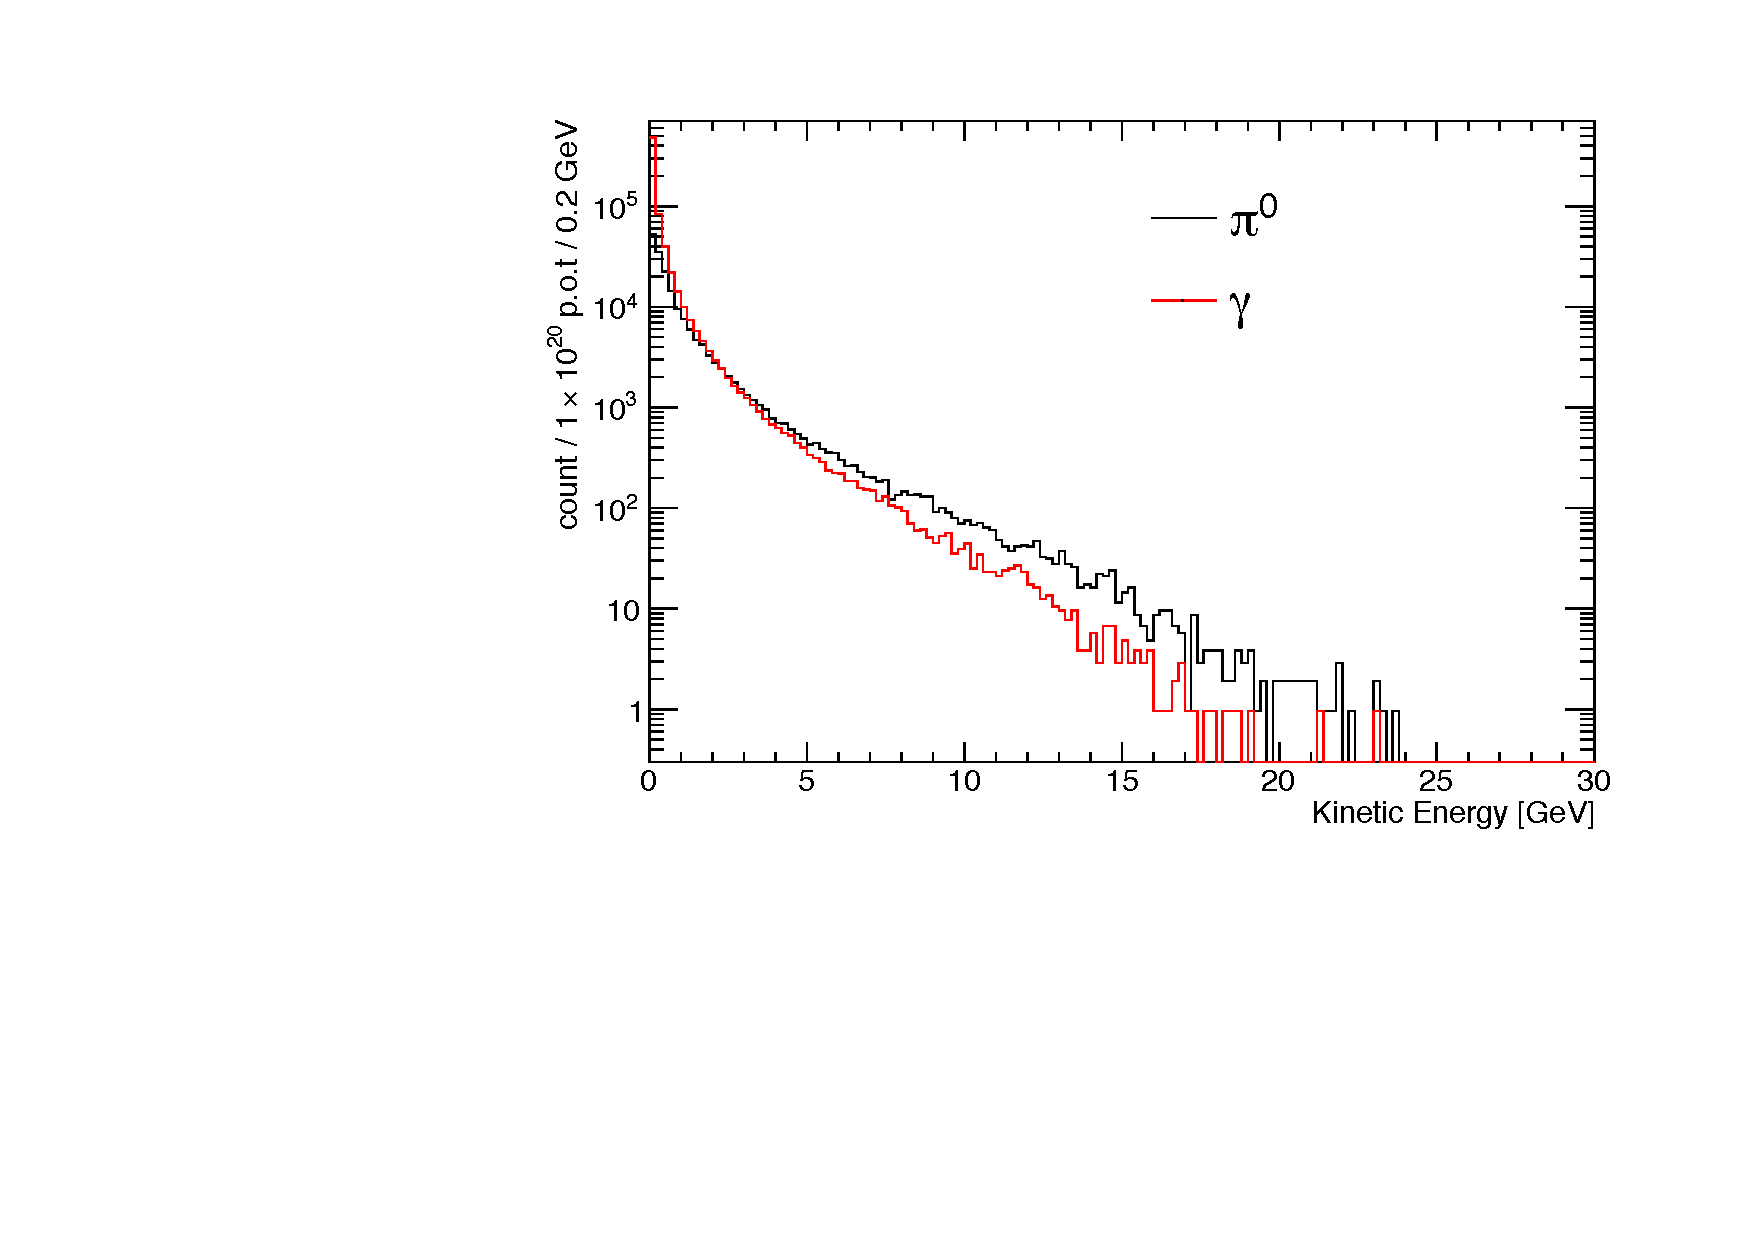
\includegraphics[width=76mm]{Chapter4/figures/piZeroAndGammaKineticEnergy.pdf}
	\caption{Left: The number of $\pi^{0}$s generated per neutrino interaction in the TPC. Right: The kinetic energy spectrum of $\pi^{0}$s originating from neutrino interactions in the TPC (black line) and the kinetic energy of the photons originating from the $\pi^{0}$s (red line). Both plots show results based on a simulations of 1 $\times$ 10$^{20}$ p.o.t.}
	\label{fig:pi0KineticEnergy}
\end{center}
\end{figure}

\subsection{Photon Energy Reconstruction}
Photons of energies ranging from 0.1 - 5 GeV are generated in the centre of the TPC, directed downstream, $\boldsymbol{\hat{p}}_{\gamma}$ = (0,0,1). Summing up the energy deposited in the TAS per photon generated then gives a relationship of the truth energy to the reconstructed energy. 10$^{4}$ photons were generated for this study with a uniform distribution over the energy range. Figure \ref{fig:photonMeanReconEnergy} shows the mean reconstructed photon energy per 0.2 GeV truth energy bin. Approximating this relationship with a linear fit represents the relationship well and yields a gradient of $\alpha$=0.568. Such that the reconstructed energy of photons within the TAS actually represents a true energy of $E_{truth} =  E_{recon}$/0.568. Applying this scale factor to the reconstructed photon energy then yields a close representation of the true reconstructed photon energy. Plotting $(E_{truth} - \alpha E_{recon})/E_{truth}$ on an event basis and fitting a Gaussian distribution of mean value $\mu$=0.01 and $\sigma$=0.37 to the peak is shown in figure \ref{fig:photonReconEnergyDiff}. 

\begin{figure}[htbp]
\begin{center}
  	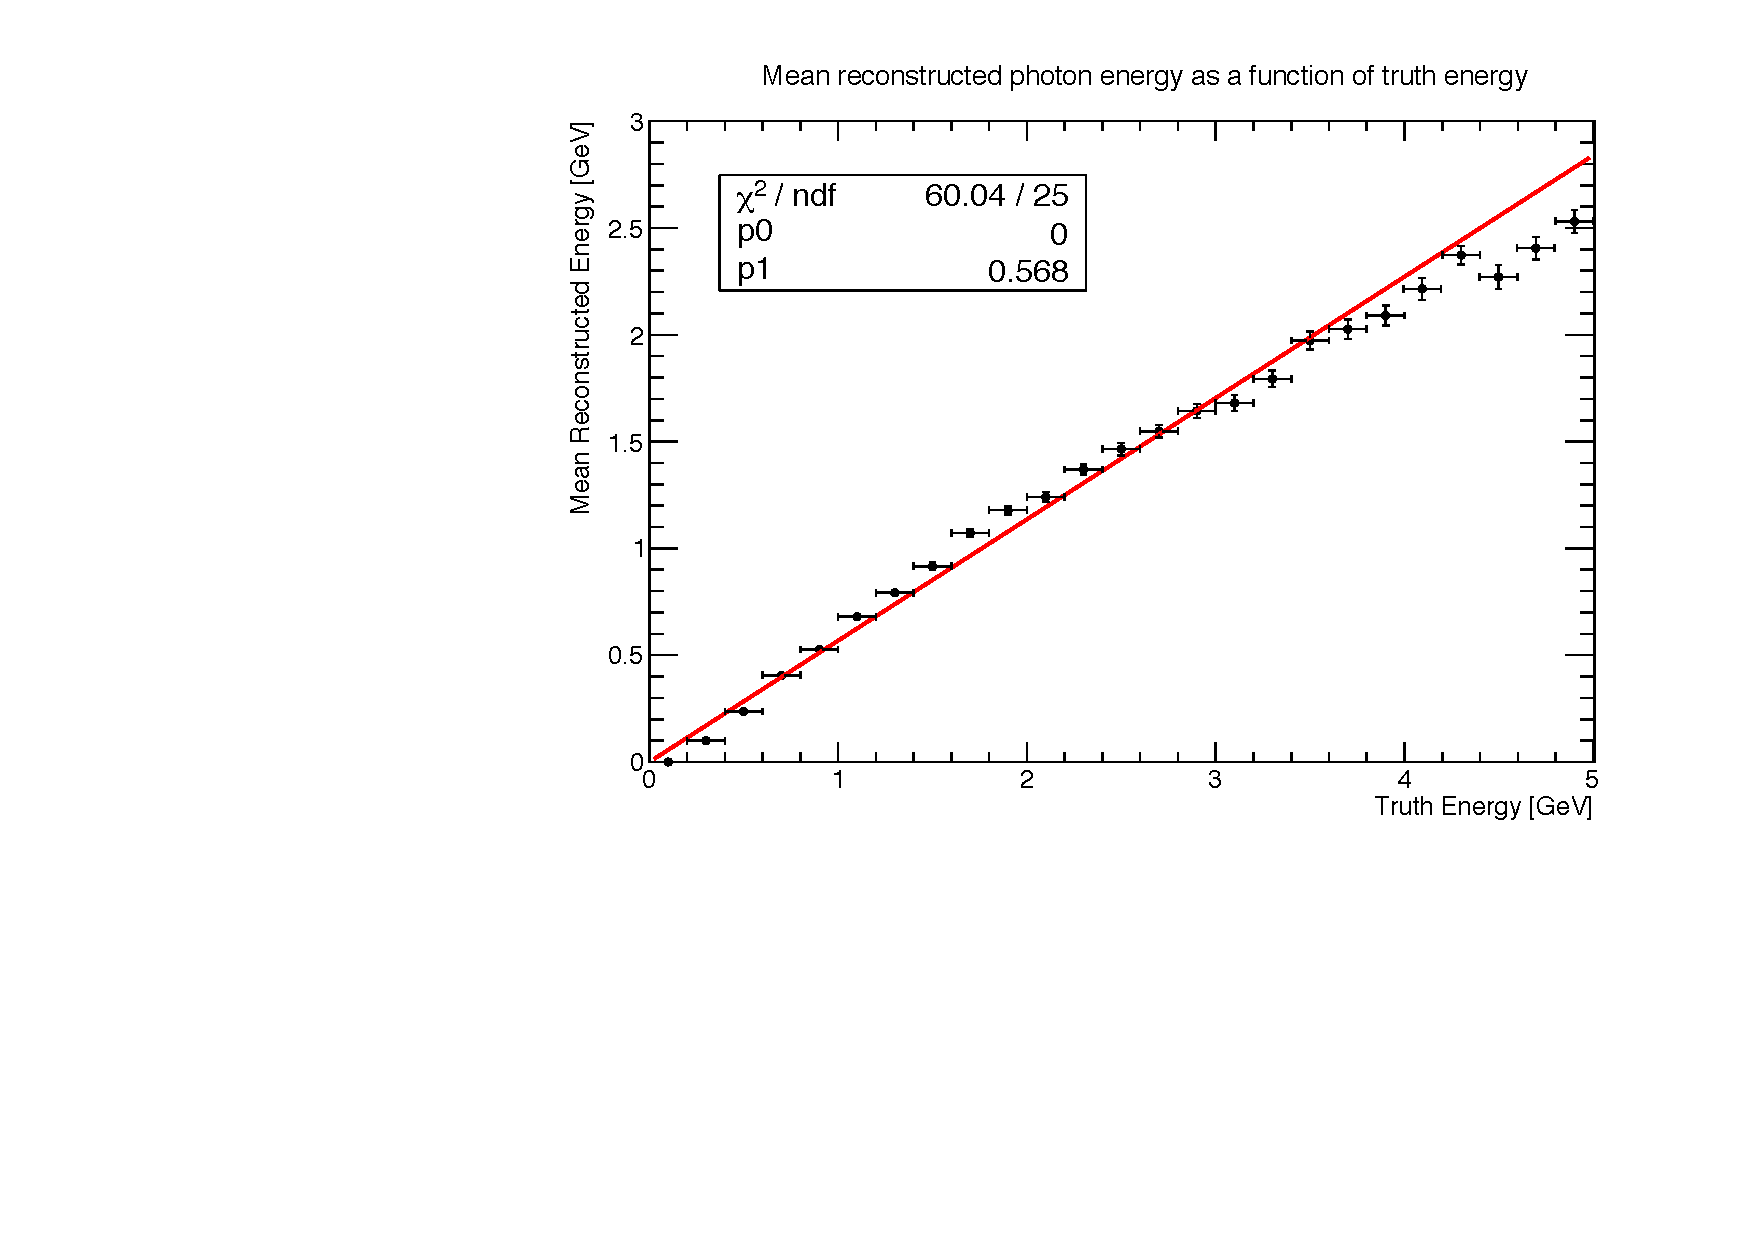
\includegraphics[width=76mm]{Chapter4/figures/testPhoton_energy_meanRecon.pdf}
  	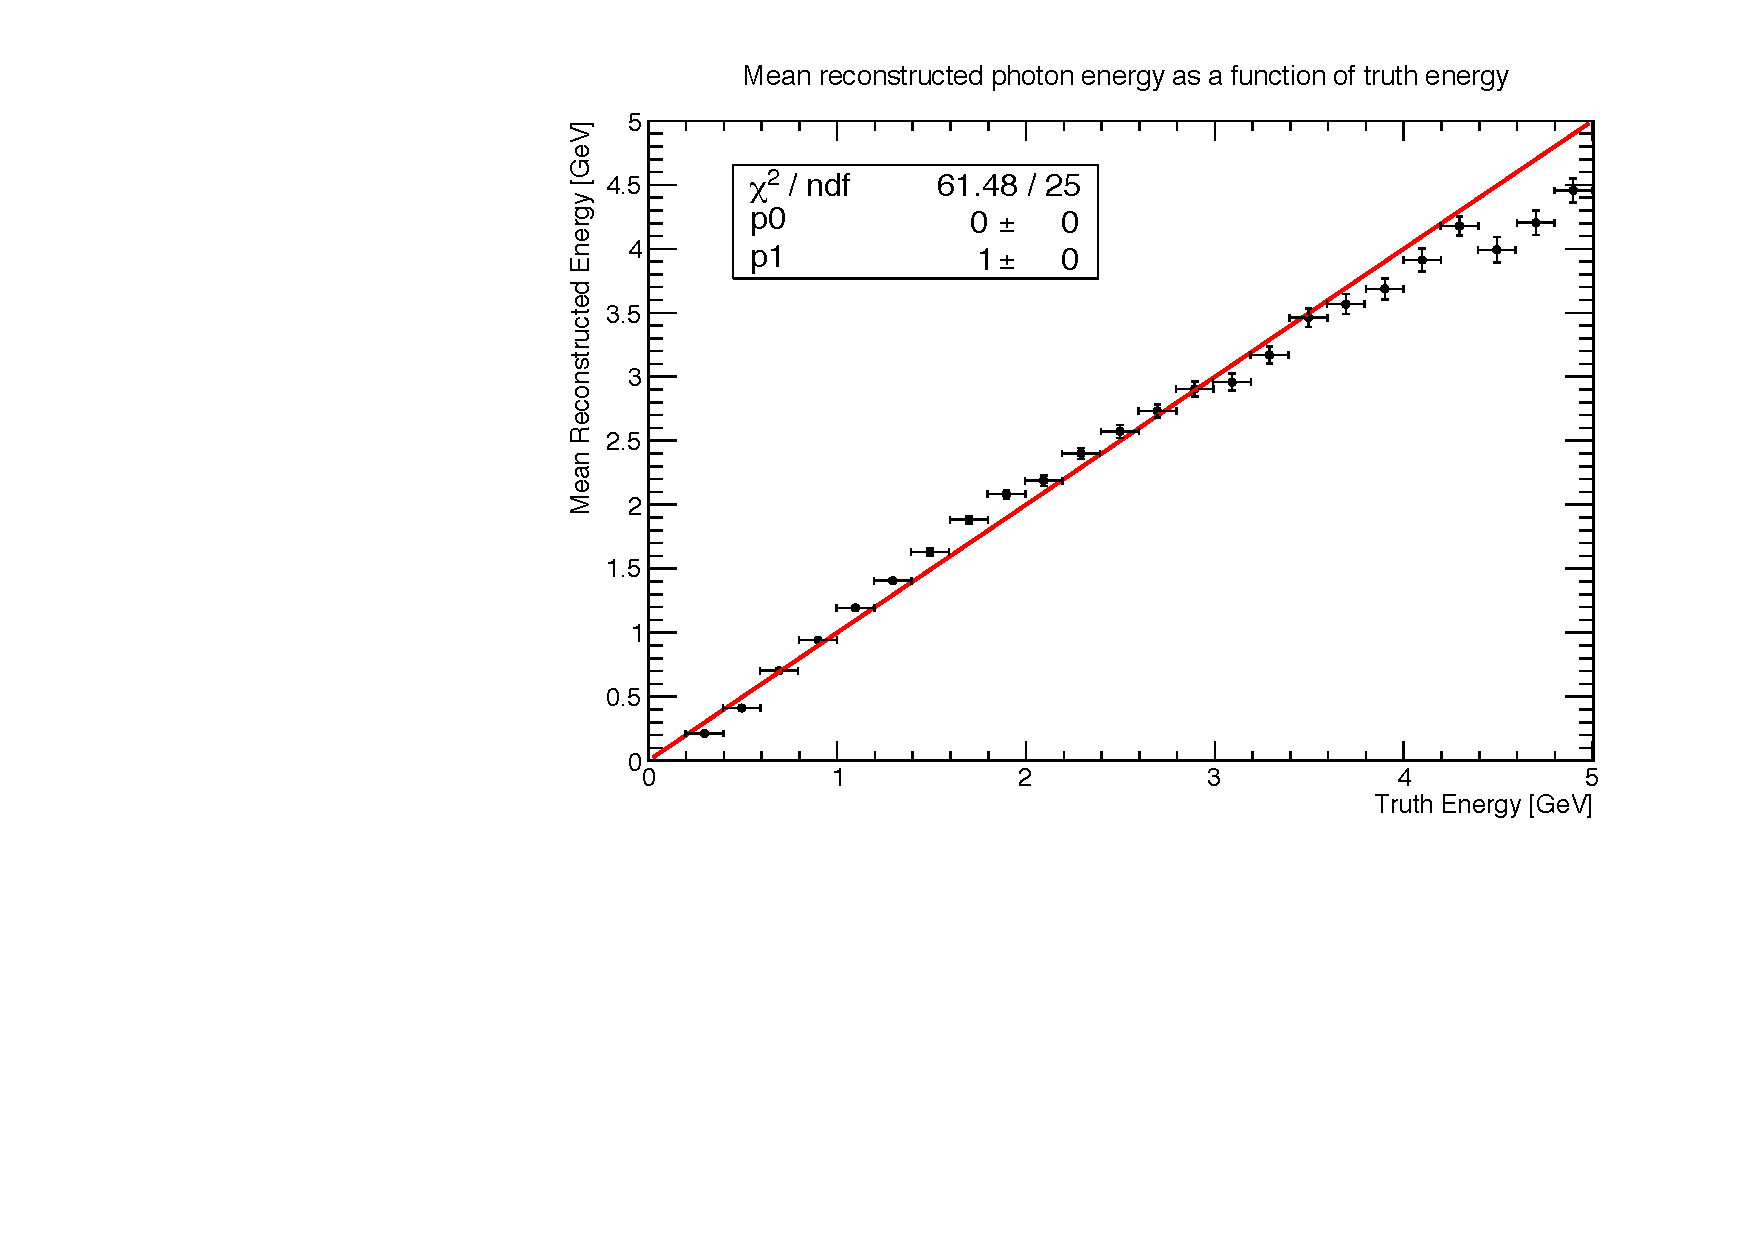
\includegraphics[width=76mm]{Chapter4/figures/testPhoton_energy_meanRecon_scaled.pdf}
		\caption{The mean reconstructed energy of photons within the TAS as a function of truth energy both before (left) and after (right) scaling. Showing linear fits with gradients of 0.568 and 1 respectively. The mean is taken per truth energy bin width of 0.2 GeV and errors bars represent the standard error on the mean. 10$^{4}$ photons were simulated within the energy range and the plots only include non zero reconstructed values, which is represented by 8734 photons.}
	\label{fig:photonMeanReconEnergy}
\end{center}
\end{figure}

\begin{figure}[htbp]
\begin{center}
  	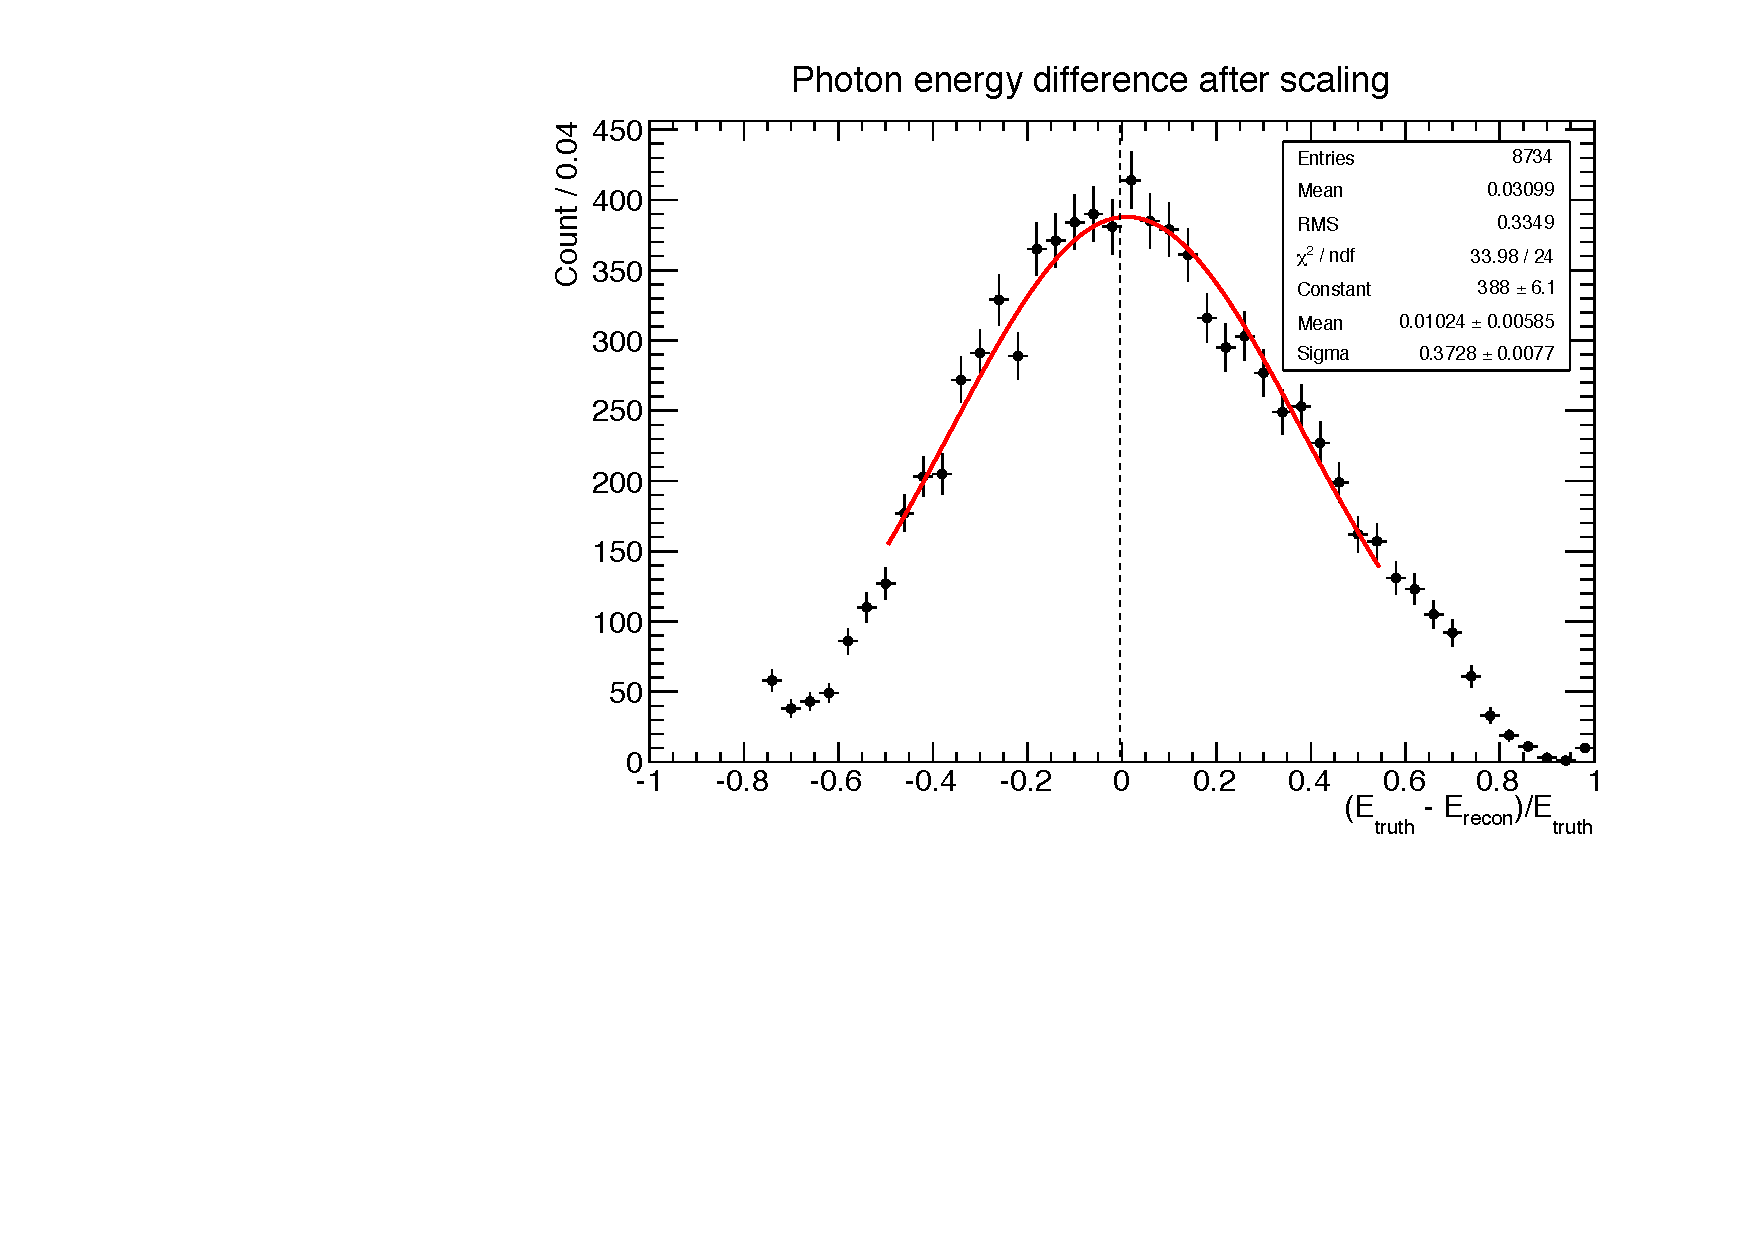
\includegraphics[width=120mm]{Chapter4/figures/testPhoton_energy_diff_plot_scaled.pdf}
		\caption{The difference between the truth and reconstructed photon energies, $(E_{truth} - \alpha E_{recon})/E_{truth}$, within the TAS after the scaling factor of $\alpha$ = 0.568 is applied. A Gaussian function is fitted to the peak of the distribution yielding a mean value of 0.01 and with a spread of 1$\sigma$ = 0.37.}
	\label{fig:photonReconEnergyDiff}
\end{center}
\end{figure}

\subsection{$\pi^{0}$ Invariant Mass}
The invariant mass of the $\pi^{0}$, $m_{\pi}$, can be determined from the photon kinematics, $m^{2}_{\pi} = p^{\mu}p_{\mu} = (q_{1} + q_{2})^{2}$, as shown in figure \ref{fig:piZeroDecay}. In the lab frame, with $E^{\gamma}_{1}$ and $E^{\gamma}_{2}$ the energies of the photons and $\alpha$ the angle between the two photons, the invariant mass squared can be determined by equation \ref{eq:piZeroMass}. The invariant mass of $\pi^{0}$ has been experimentally measured and has a well established result of $m_{\pi}$ = 134.98 MeV \cite{pionDecayModes}. Matching photon pairs to produce an invariant mass close to this value, using equation \ref{eq:piZeroMass}, can then indicate the photons originated from a $\pi^{0}$ with energy $E_{\pi} = E^{\gamma}_{1} + E^{\gamma}_{2}$.

\begin{equation}
	m^{2} = 4E^{\gamma}_{1}E^{\gamma}_{2}\textnormal{sin}^{2}\big(\frac{\alpha}{2} \big)
	\label{eq:piZeroMass}
\end{equation}

\begin{figure}[htbp]
\begin{center}
  	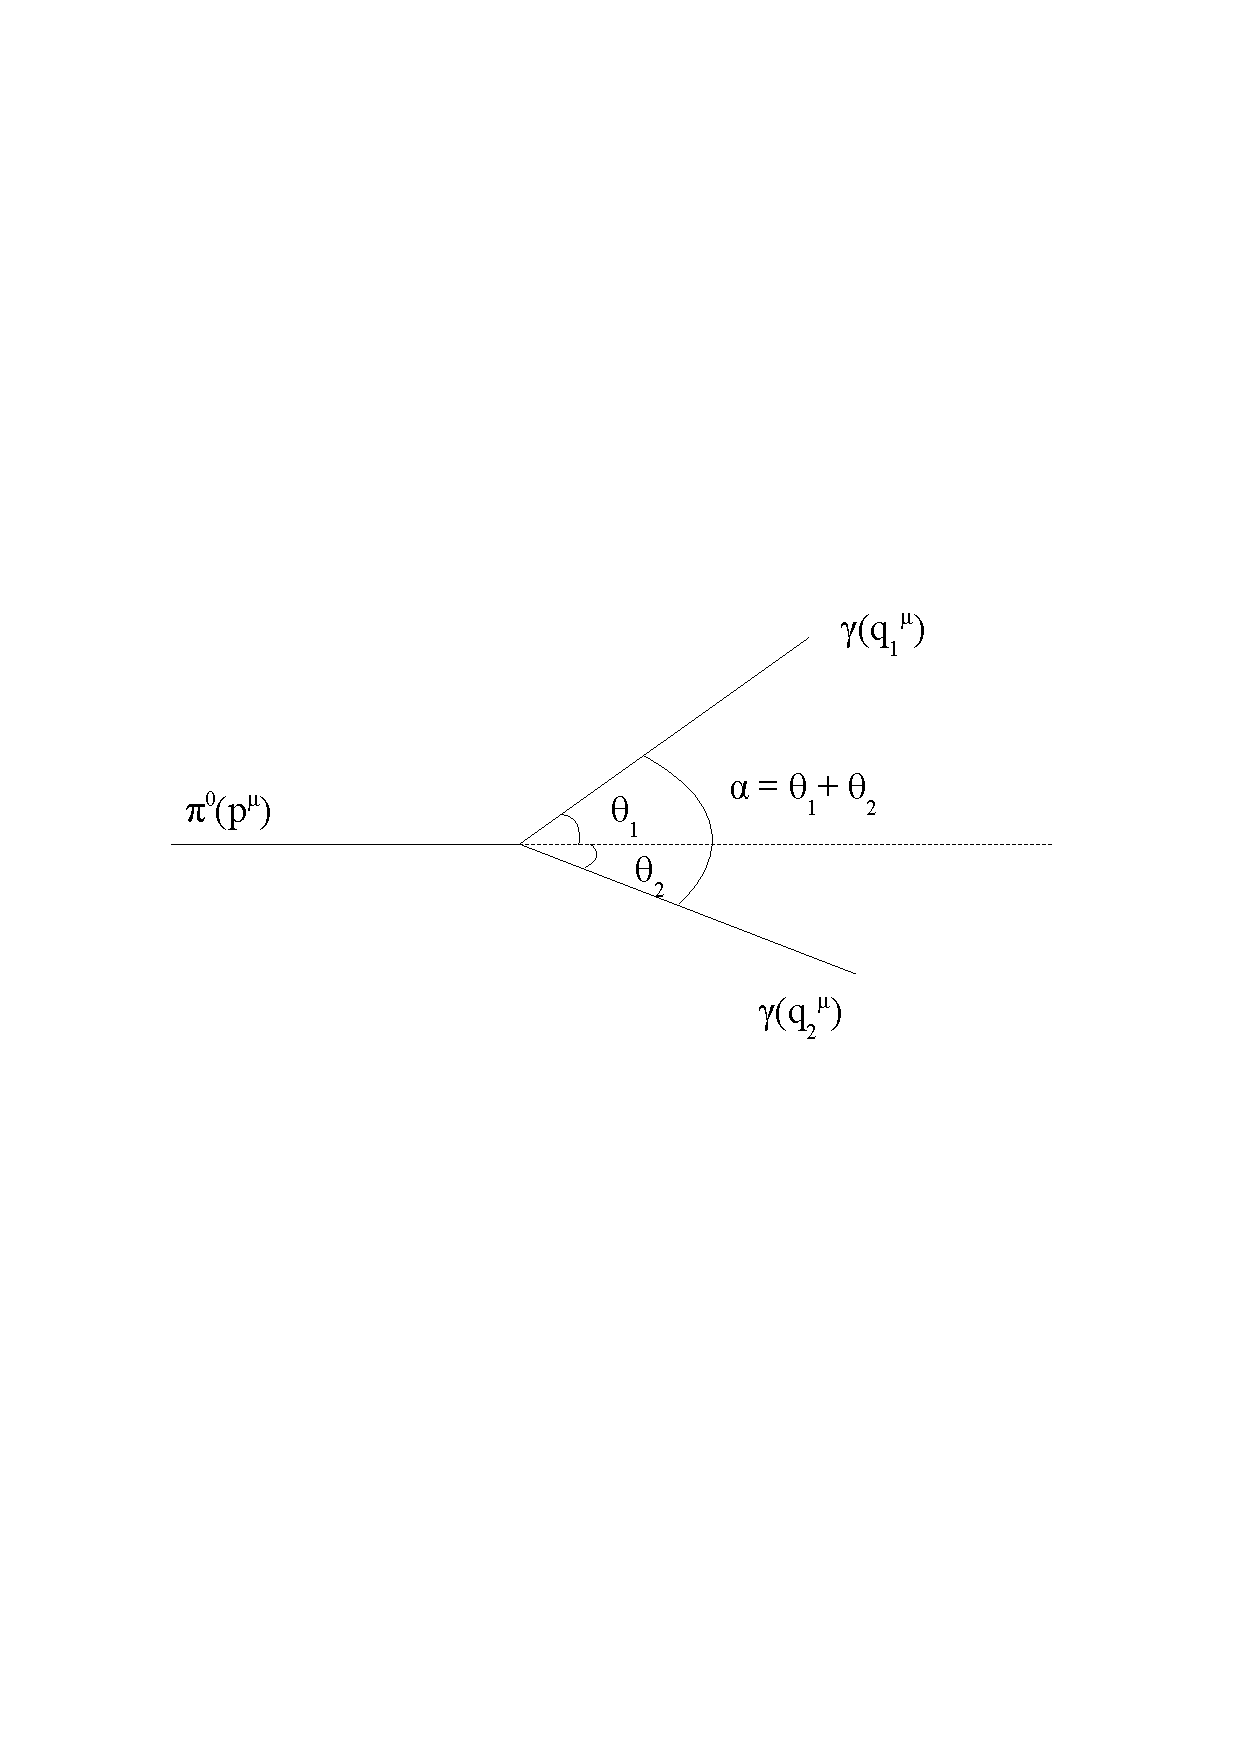
\includegraphics[width=120mm]{Chapter4/figures/piZeroDrawing.pdf}
		\caption{An illustration of a $\pi^{0}$ of 4-momentum $p^{\mu}$ decaying into two photons of momentums $q_{1}^{\mu}$ and $q_{2}^{\mu}$ separated by an angle $\alpha$ in the lab frame.}
	\label{fig:piZeroDecay}
\end{center}
\end{figure}

Similar MC experiments to the photon tests were conducted also within the TAS to determine how well the invariant mass of single $\pi^{0}$s could be reconstructed. With an energy distribution of 0.2 - 10 GeV and momentum purely in the beam direction 10$^{4}$ $\pi^{0}$s were generated in the centre of the TPC. Tracking each outgoing photon and recording only hit information, the invariant mass is then calculated from equation \ref{eq:piZeroMass}. The energy of each photon is given by the sum of the total energy deposition along its trajectory, $E^{\gamma}_{i}$ = $\sum^{hits}_{n}{E^{deposited}_{n}}$. The momentum of each outgoing photon is determined from the truth values.
%by the straight line between the decay vertex location (truth information) and the initial hit position within the TAS. By process of the scalar product of these two 3 unit vectors, $\boldsymbol{\hat{p}}_{1}$$\cdot$$\boldsymbol{\hat{p}}_{2}$ = cos$\alpha$, a measurement of the angle between the two photons is made.
Photons which deposit no energy cannot provide a measurement of the invariant mass and are discounted. Other decay modes of $\pi^{0}$s are ignored from this study. An implicit photon energy cut of 50 MeV is applied to remove poorly reconstructed photon tracks, requiring both outgoing photons to have reconstructed energies above this threshold.

The effect of the reconstructed angle on the invariant mass is large and due to this no reconstruction on the angle is performed, with truth values for the photon momentum being used instead. To fully estimate the detectors potential of measuring $\pi^{0}$s this effect needs to be studied further as it depends on the $\pi^{0}$ vertex location and hit locations of the 2 photons in the TAS, which are limited by track reconstruction and the position resolution in both the TPC and the TAS.

The reconstructed invariant mass can be seen in figure \ref{fig:piZeroReconMassUnscaled} without any scaling applied to the energies of the outgoing photons. A Gaussian distribution of $\mu$=82.5 MeV and $\sigma$=27.8 MeV is fitted in the region of 45 to 125 MeV. This is far lower than the expected $\pi^{0}$ mass but upon scaling with the factor determined from fits to previous photon simulation data of $\alpha$=0.568, taken from figure \ref{fig:photonMeanReconEnergy}, a mean value of 143.8 MeV is determined from a similar fitting. The mean of the data is even closer to the true value at 135.7 MeV. However such scaling introduces a larger spread over the distribution and has an increased standard deviation of 48.2 MeV. The experimentally determined value of 134.98 MeV then lies well within 1 standard deviation of the fitted mean value. 

The energy difference between the truth and the reconstructed values of the $\pi^{0}$s generated conforms well with a Gaussian distribution, both for pre and post scaling data sets. Figure \ref{fig:piZeroReconEnergyDiff} illustrates the differences from determination of the quantity (E$_{truth}$ - E$_{recon}$)/E$_{truth}$.

\begin{figure}[htbp]
\begin{center}
  	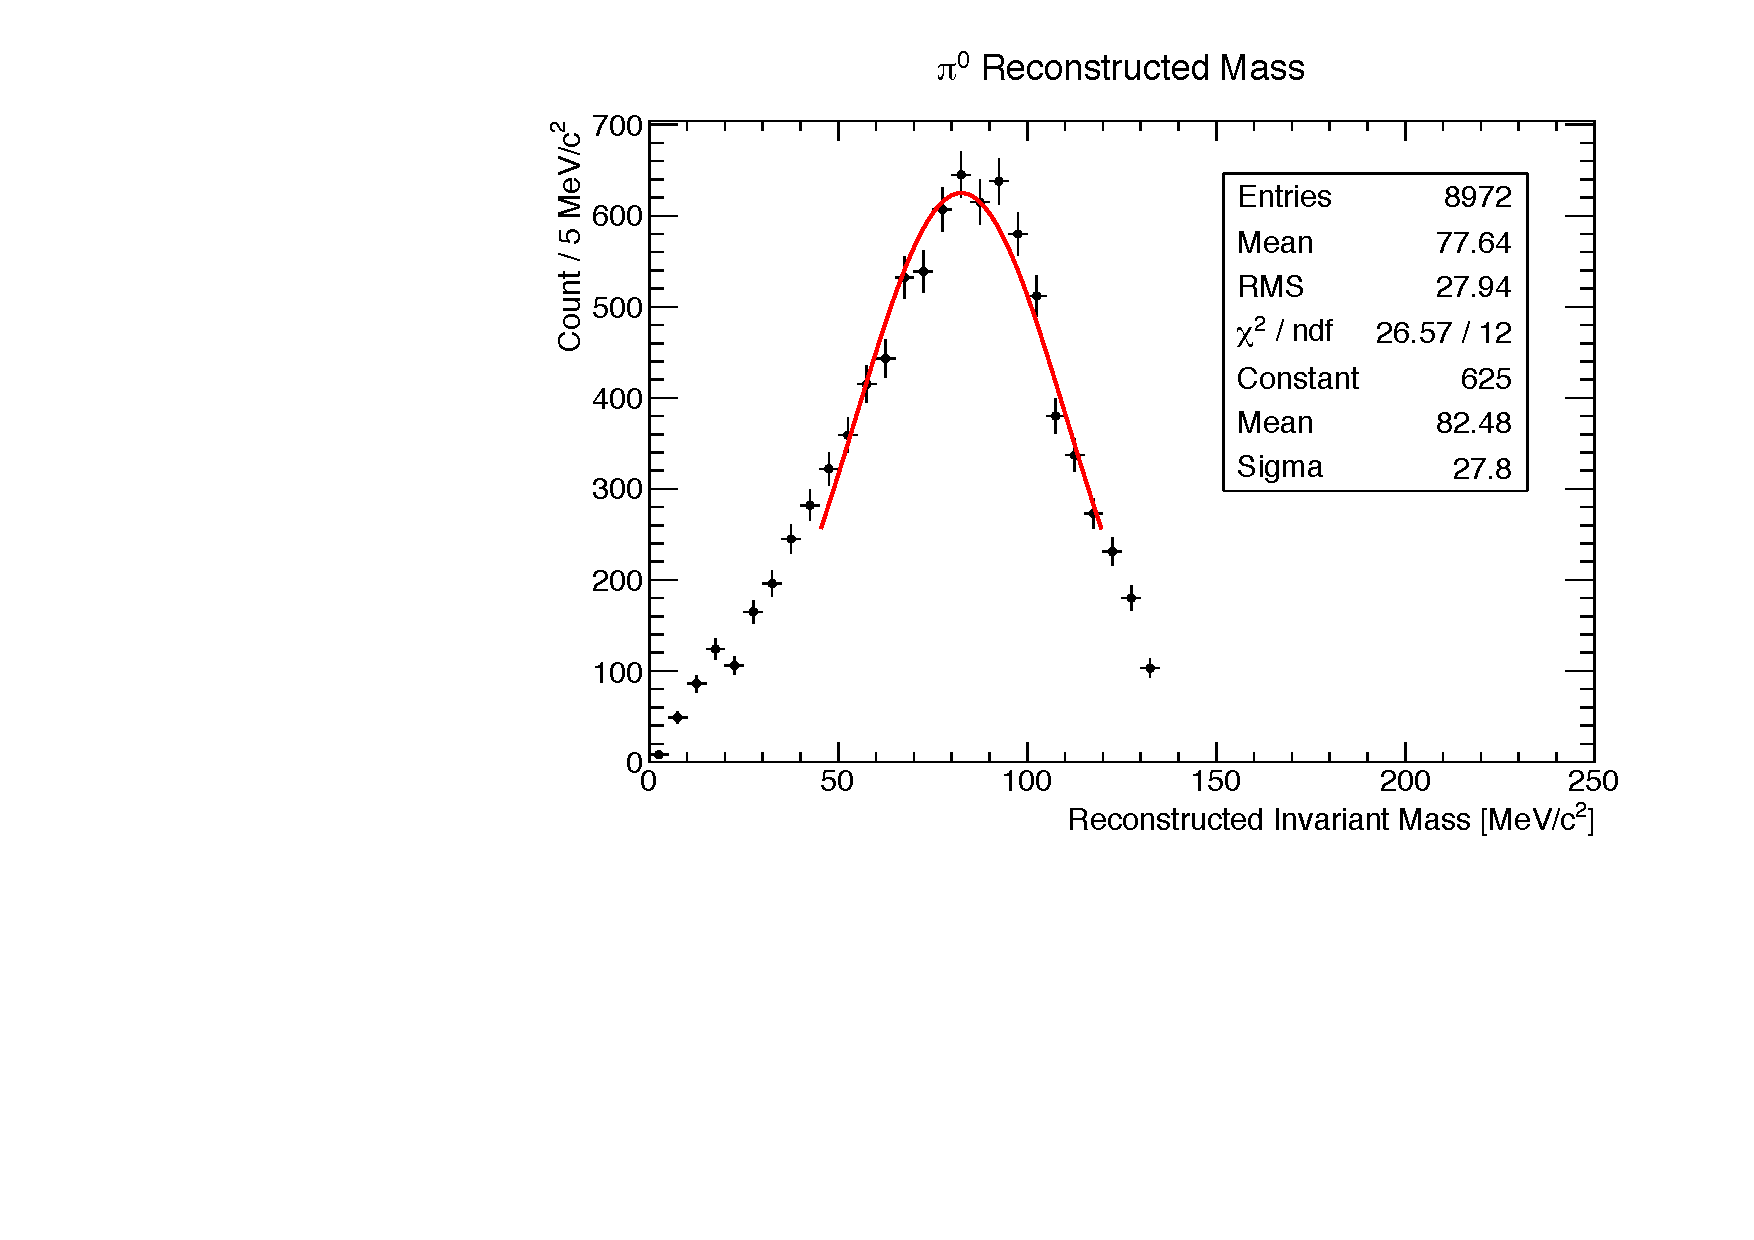
\includegraphics[width=76mm]{Chapter4/figures/piZeroReconMassUnscaledNoCuts.pdf}
  	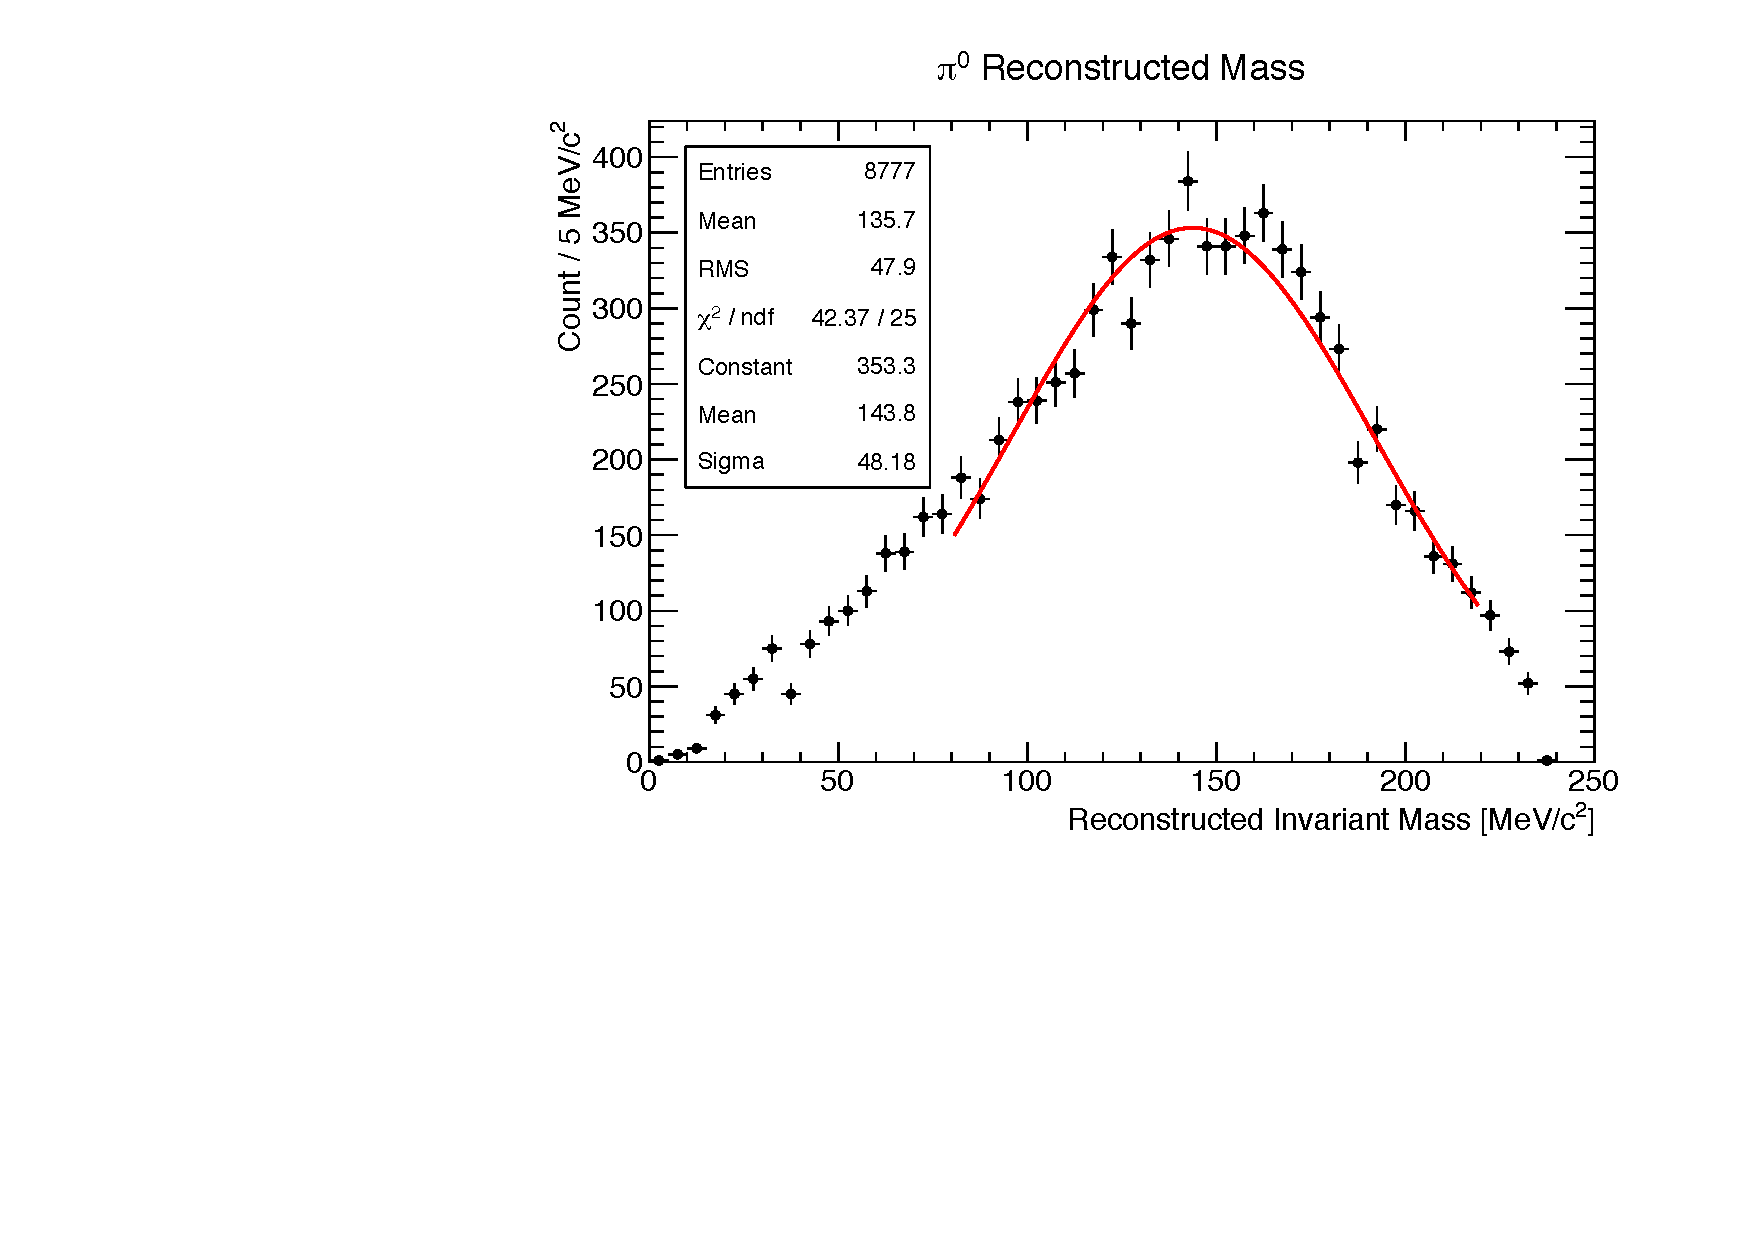
\includegraphics[width=76mm]{Chapter4/figures/piZeroReconMassScaledNoCuts.pdf}
		\caption{The invariant mass of $\pi^{0}$s generated within the TPC using the energy deposition within the TAS to reconstruct the energy of each outgoing photon. Truth values of the separation angle in the lab frame are used in the reconstruction of the mass. Left: Unscaled photon energies. Right: Scaled photon energies by a factor of $\alpha^{-1}$=1.76.}
	\label{fig:piZeroReconMassUnscaled}
\end{center}
\end{figure}

\begin{figure}[htbp]
\begin{center}
  	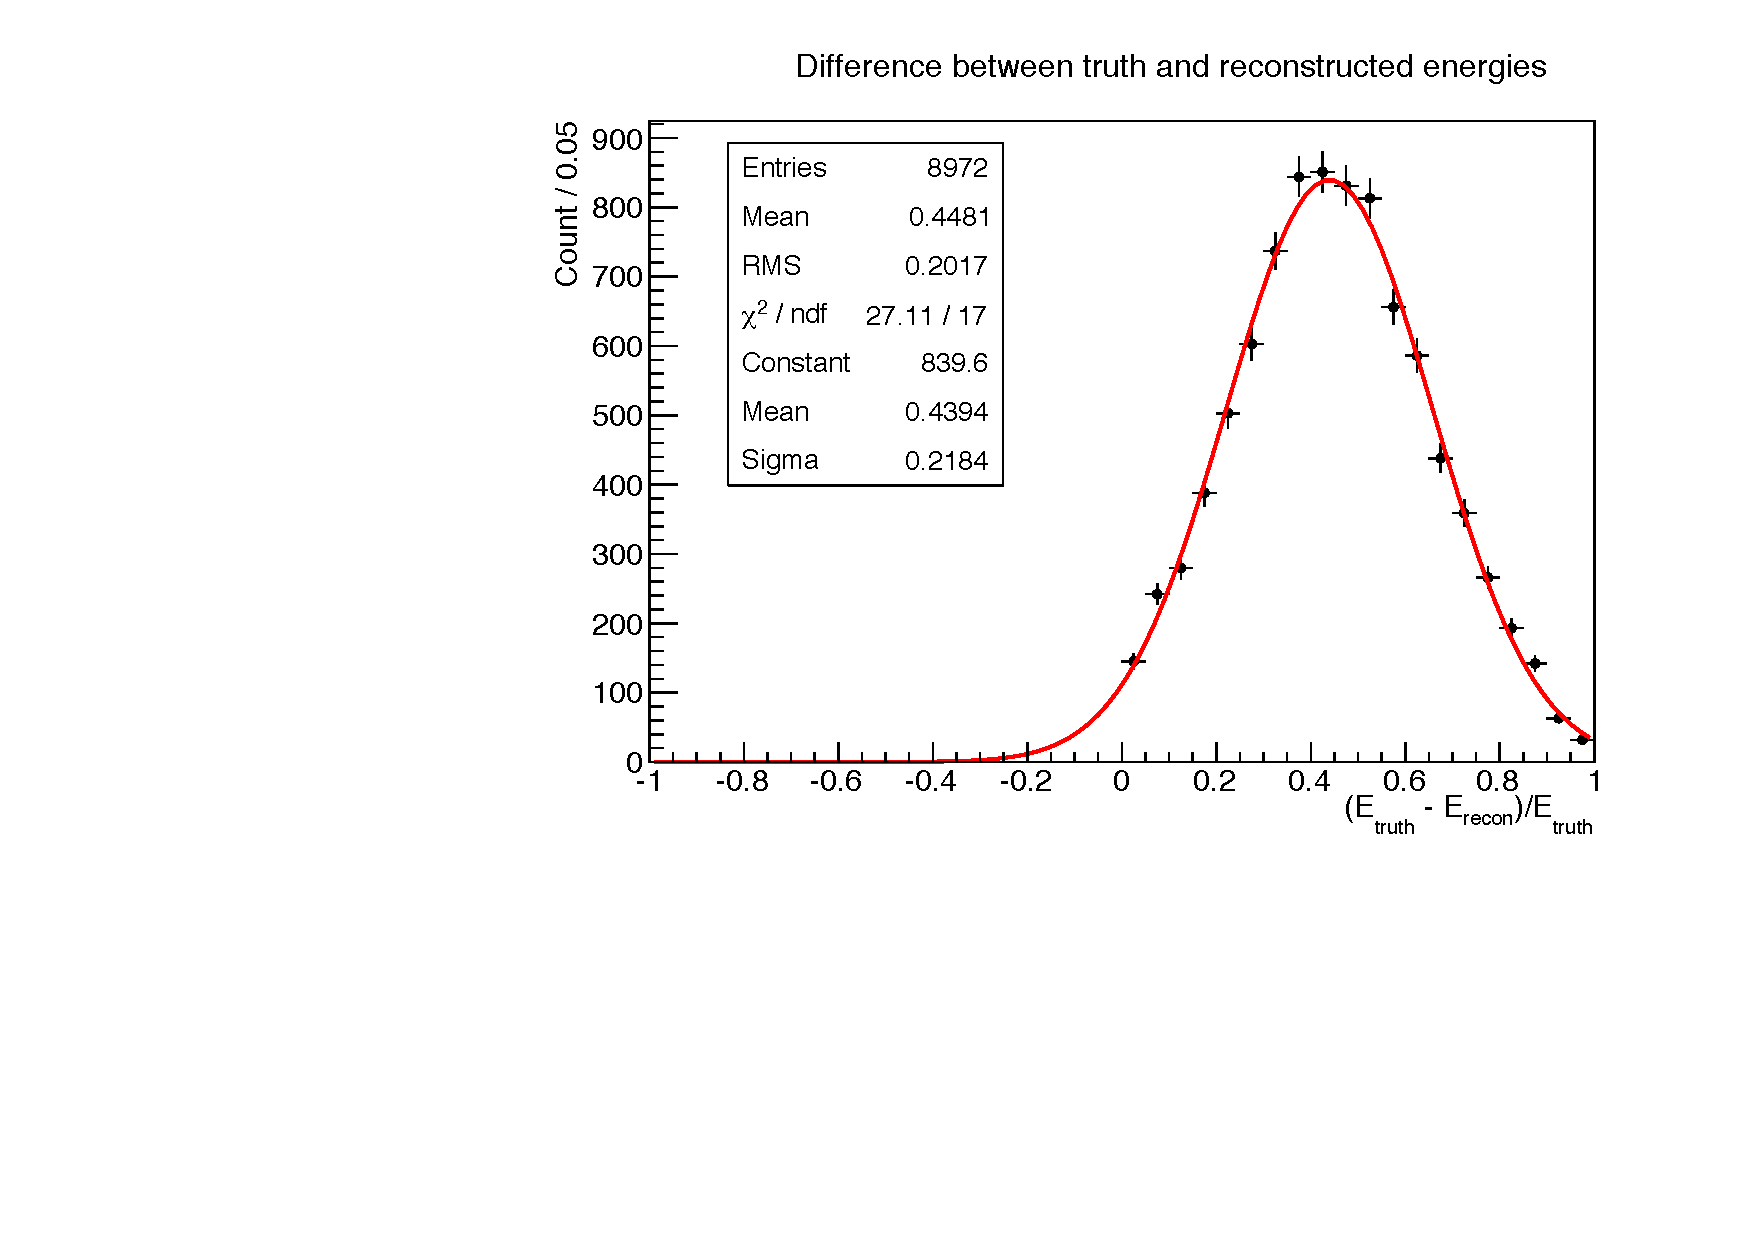
\includegraphics[width=76mm]{Chapter4/figures/piZeroEnergyDiffUnscaledNoCuts.pdf}
  	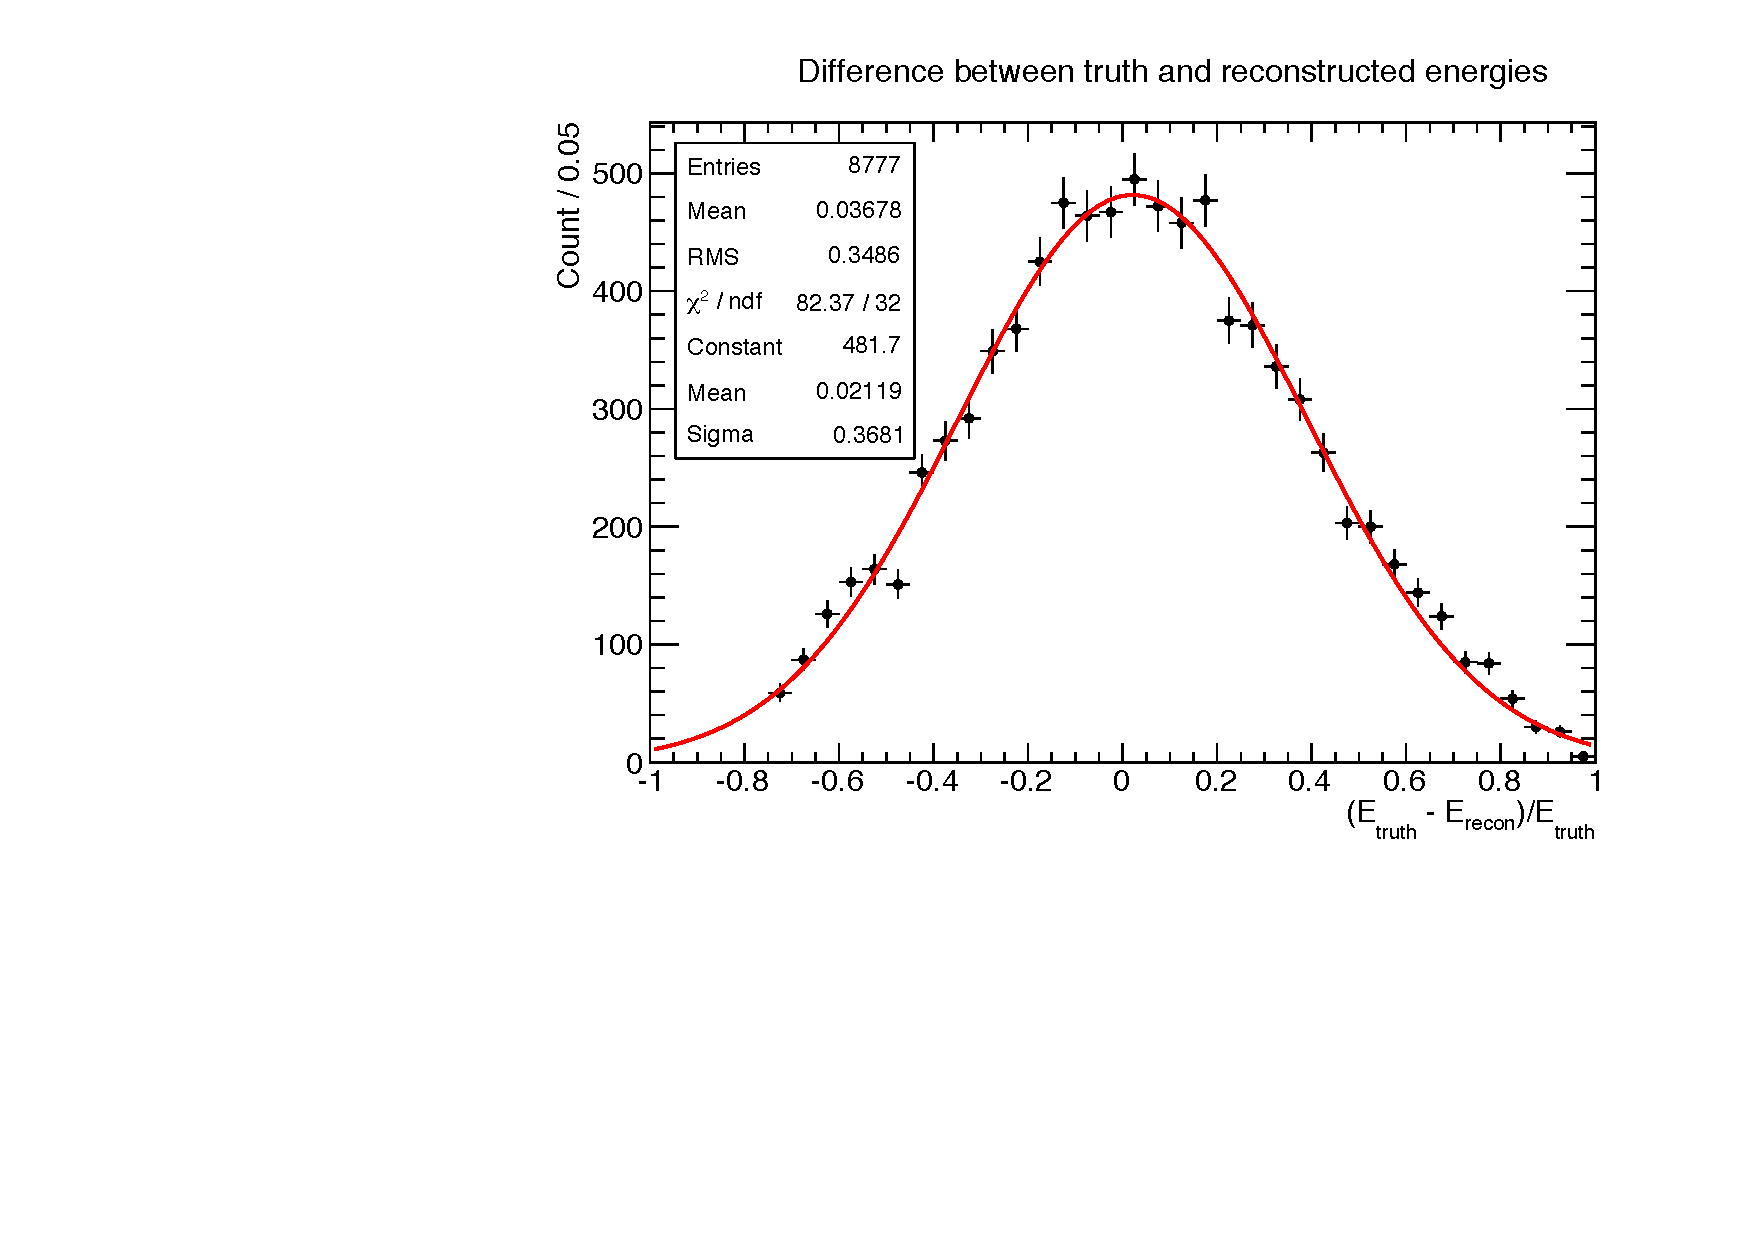
\includegraphics[width=76mm]{Chapter4/figures/piZeroEnergyDiffScaledNoCuts.pdf}
		\caption{The difference between the truth and reconstructed energies of $\pi^{0}$s generated in the TPC. Left: Unscaled photon energies. Right: Scaled photon energies by a factor of $\alpha^{-1}$=1.76.}
	\label{fig:piZeroReconEnergyDiff}
\end{center}
\end{figure}

The lower energy photons contribute to the spreading of the distribution and it can be seen that adding more stringent selections on the photons tracks leads to a more precise value of the reconstructed mass. Requiring at least 4000 hits on each outgoing photon yields a better measurement on the reconstructed mass once fitted with a Gaussian distribution with a mean value of 134.9 MeV, as shown in figure \ref{fig:piZeroReconMassWithCuts}. However the number of $\pi^{0}$s passing this selection is then reduced to 42.5\%.

\begin{figure}[htbp]
\begin{center}
  	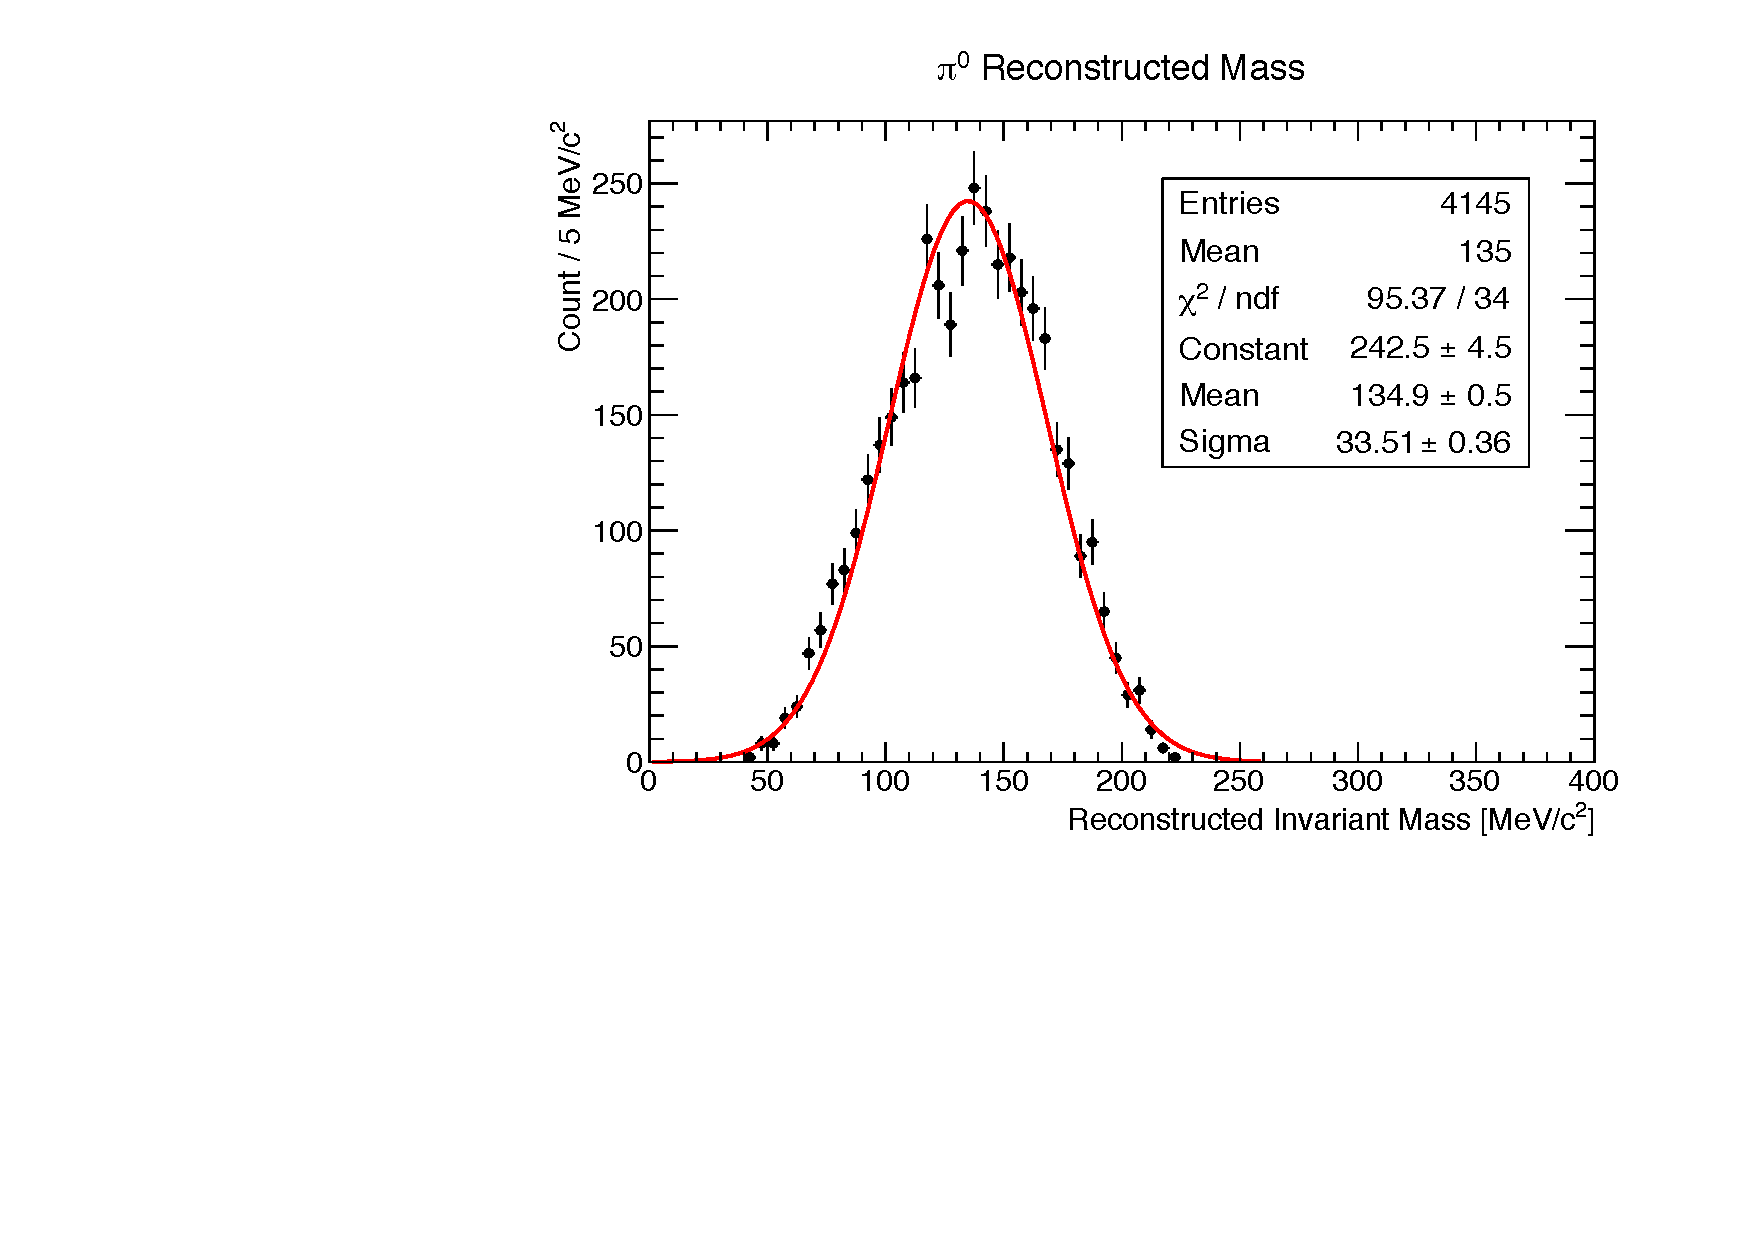
\includegraphics[width=100mm]{Chapter4/figures/piZeroReconMassScaled_4000HitCut_0o05GeVcut.pdf}
		\caption{The invariant mass of $\pi^{0}$s generated within the TPC using the energy deposition within the TAS to reconstruct the energy of each outgoing photon. Truth values of the separation angle in the lab frame are used in the reconstruction of the mass. Each outgoing photon energy is scaled by factor $\alpha^{-1}$=1.76 and only photons with 4000 hits per track are included.}
	\label{fig:piZeroReconMassWithCuts}
\end{center}
\end{figure}

%\begin{figure}[htbp]
%\begin{center}
%  	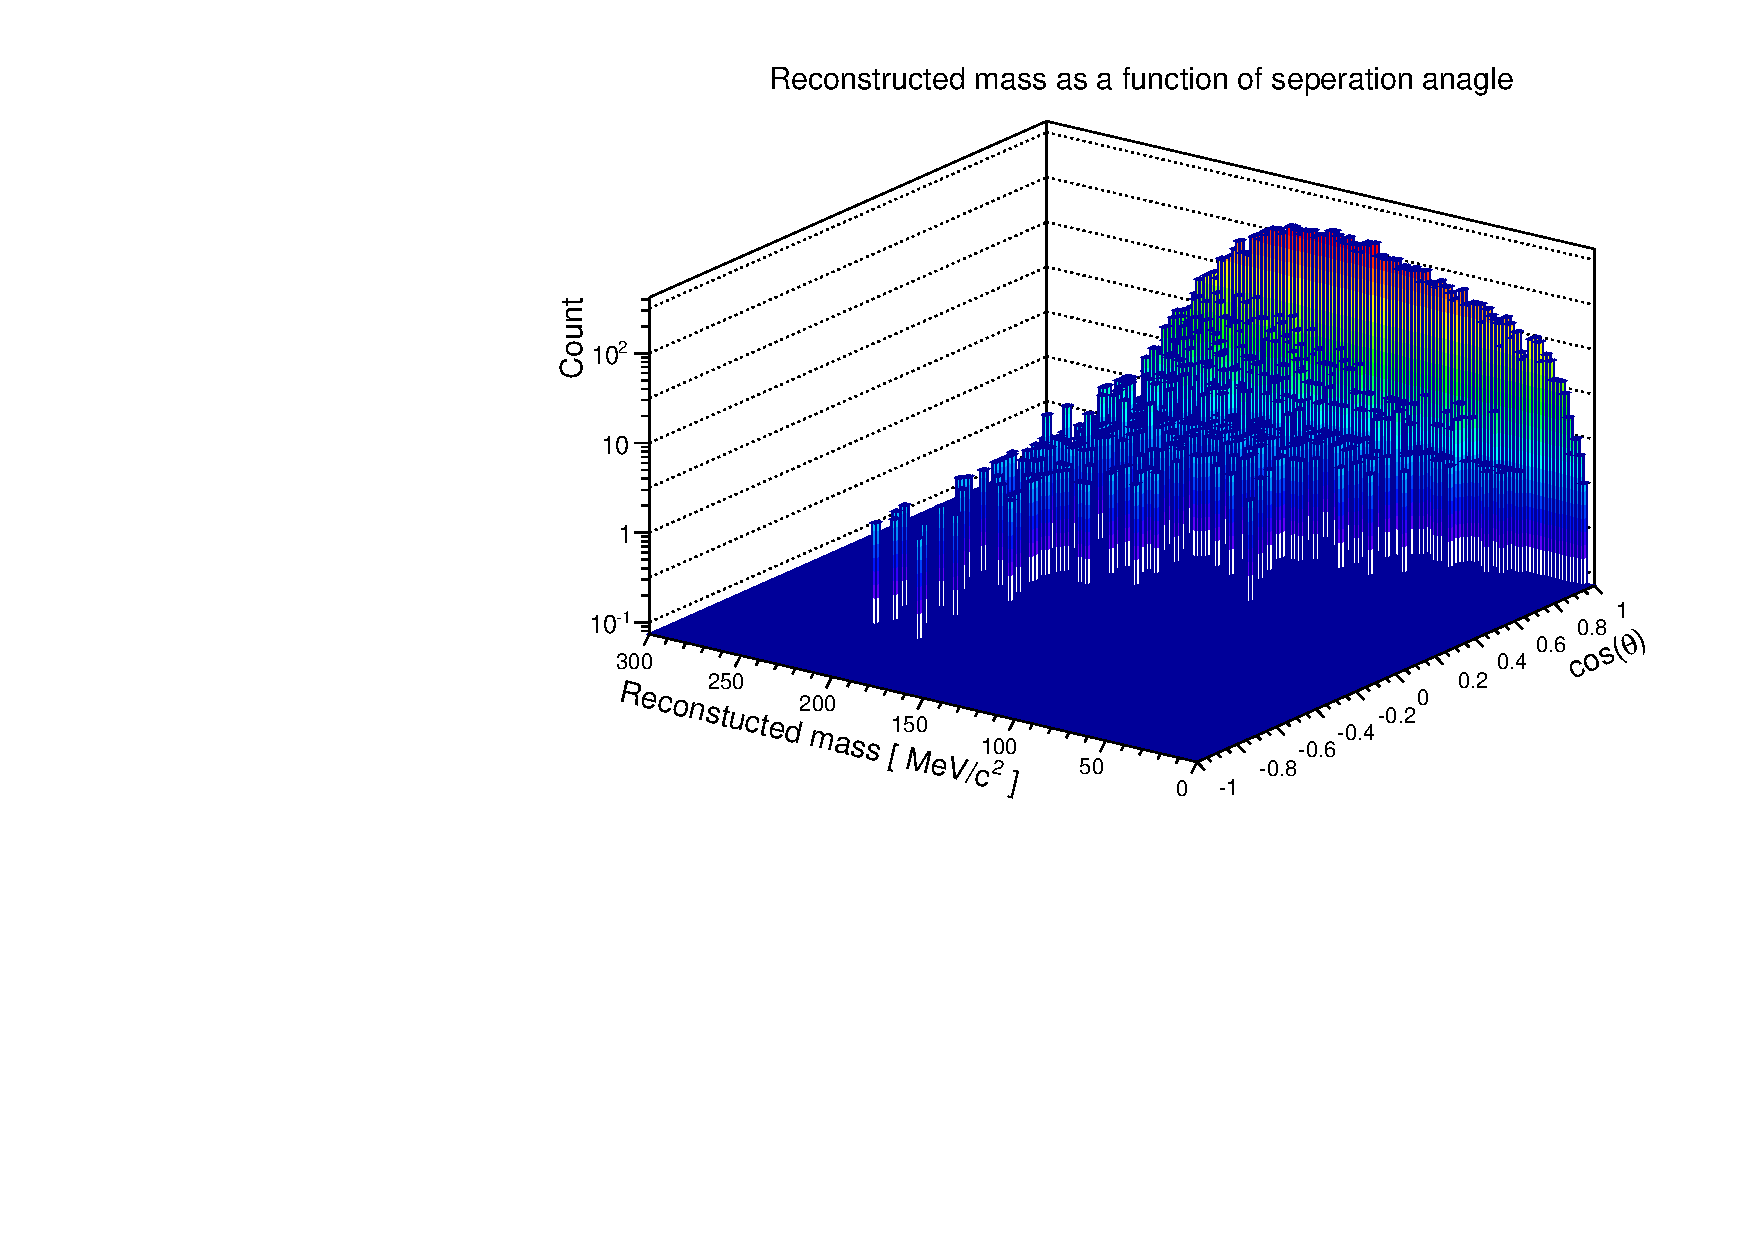
\includegraphics[width=120mm]{Chapter4/figures/piZeroReconMassScaledVsAngle_NoCuts_3D.pdf}
%		\caption{The reconstructed mass of $\pi^{0}$s as a function of the cosine of the speration angle between the two outgoing photons.}
%	\label{fig:piZeroReconMassVsAngle}
%\end{center}
%\end{figure}

%\section{A Combined Neutrino Energy Reconstruction within the TPC and TAS}
%The results from the previous study show energy reconstruction of $\pi^{0}$s using the TAS is possible. A combined analysis on the energy reconstruction of neutrinos is then implemented using both the TPC and the TAS. The TAS will then provide information solely on $\pi^{0}$s originating from the neutrino vertex.
%
%Based on results from the previous studies, scaling the secondary photon energies by the factor of $\alpha^{-1}$=1.76 arose as the best linear between the truth and mean reconstructed energies of $\pi^{0}$s. The total energy deposited in the TAS from photon interactions is then simply the sum of the energy deposition scaled by this factor. Truth information on the particle is used such that only energy deposition from photons is included, neutrons are excluded. The total reconstructed neutrino energy is then given more accurately by equation \ref{eq:totalNuMom4}, which extends equation \ref{eq:totalNuMom3} to include the contribution from the TAS. The first term in this equation relates to momentum measurements within the TPC and the second term is then the contribution from energy calorimetry from the TAS layer for photons. $\Delta{E_{i}}$ corresponds to the amount of energy deposited by each hit in the TAS originating from a photon interaction. 
%
%\begin{equation}
%	E_{\nu} \approx c\sum^{N_{tracks}}_{i}{p^{trans}_{i}} + \sum^{N_{hits}}_{i}{\Delta{E_{i}}}
%	\label{eq:totalNuMom4}
%\end{equation}
%
%The majority of the incident neutrino energy is transferred to charged particles in CC interactions and to the neutrino in NC interactions, whereas the contribution from photons is low in respect. Due to this the second term is not expected to contribute very largely to the reconstruction. The previous figure \ref{fig:neutrinoMomReconVsTruth} shows the reconstructed neutrino energy without the TAS contribution as a function of truth energy on an event by event basis.The addition of the TAS contribution is then shown in figure \ref{fig:neutrinoMomReconFull}.
%
%\begin{figure}[htbp]
%\begin{center}
%  	\includegraphics[width=74mm,height=50mm]{Chapter4/figures/recon_truthVsReconMom_neutrino_with_pi0.pdf}
%	\includegraphics[width=74mm,height=48mm]{Chapter4/figures/mean_recon_neutrino_energy_all_with_pi0.pdf}
%	\caption{Left: The reconstructed neutrino momentum as a function of the truth neutrino momentum for all (CC + NC) interactions types, also instrumenting the TAS layer. Right: The mean reconstructed neutrino energy as a function of truth neutrino energy. The mean reconstructed value is determined from all events that fall within each 0.5 GeV truth bin. Error bars indicate the standard deviation value of the mean, 1$\sigma$. Results are based on simulation of exposure 9.6 $\times$ 10$^{19}$ p.o.t. }
%	\label{fig:neutrinoMomReconFull}
%\end{center}
%\end{figure}
%
%Isolating the neutrino energy reconstruction to just CC events shows large improvement using this technique, with the mean reconstructed energy coherent with the truth neutrino energy over the full energy range of 0-10 GeV. Figure \ref{fig:neutrinoMomReconCCFull} shows the final results from this reconstruction.
%
%\begin{figure}[htbp]
%\begin{center}
%  	\includegraphics[width=74mm,height=50mm]{Chapter4/figures/recon_truthVsReconMom_neutrino_with_pi0_cc.pdf}
%	\includegraphics[width=74mm,height=48mm]{Chapter4/figures/mean_recon_neutrino_energy_all_with_pi0_cc.pdf}
%	\caption{Left: The reconstructed neutrino momentum as a function of the truth neutrino momentum for CC interactions types, also instrumenting the TAS layer. Right: The mean reconstructed neutrino energy as a function of truth neutrino energy for CC events. The mean reconstructed value is determined from all events that fall within each 0.5 GeV truth bin. Error bars indicate the standard deviation value of the mean, 1$\sigma$. Results are based on simulation of exposure 9.6 $\times$ 10$^{19}$ p.o.t. }
%	\label{fig:neutrinoMomReconCCFull}
%\end{center}
%\end{figure}

\section{Estimating the Detector Performance}
We finally try to estimate the ND performance based on the initial studies presented in this chapter. In order to so the main detector systematics are estimated and show how these contribute to the signal event normalisation uncertainty and the beam $\nu_{e}$ normalisation uncertainty. This study is based on an analysis using only CC interactions in the TPC fiducial volume, selecting events where the muon vertex is located within the fiducial volume and subsequently leaves the TPC. The relative difference of the transverse $\mu^{-}$ momentum to the $\nu_{\mu}$ momentum in the TPC (truth values) as a function of the angle with respect to the beam axis is shown in figure \ref{fig:muonTransMomDiffRatioVsCosTheta} for these events to give a handle on how the muon flux represents the neutrino flux. It is clear from the figure that the majority of the muons are extremely forward going, with 56\% of muons having a $\cos{\theta}$ value exceeding 0.98. From measurement of the muon direction, and hence angle, we can then impose a selection on the muons in the TPC to provide a closer representation of the true neutrino flux. Imposing a selection on smaller angles, $\cos{\theta}$ $>$ 0.998, 44.9\% muons then are within 10\% of the truth neutrino momentum. Based on this we then use the transverse momentum of the muon to give an indication of the $\nu_{\mu}$ flux at the near detector. This aims to provide a first order estimation of the ND performance by directly looking at event rates, giving us the uncertainty on the flux $\times$ cross section which is used when extrapolating to the FD. For further, more accurate estimations of the neutrino flux from the muons we would impose these $\cos{\theta}$ selections with a hadronic cut to remove events that give poor estimation on the neutrino momentum. These are not realised in this analysis but are mentioned to motivate the use of the outgoing muon to provide a handle on the incident neutrino flux on the TPC.

\begin{figure}[htbp]
\begin{center}
  	\includegraphics[width=120mm]{Chapter4/figures/trans_muon_mom_ratio_vs_cosTheta.pdf}
	\caption{The relative difference of the transverse $\mu^{-}$ momentum to the $\nu_{\mu}$ momentum in the TPC (truth values) as a function of the angle with respect to the beam axis for $\nu_{\mu}$ CC events in the TPC fiducial volume. The total number of events based on a simulation of exposure 9.6 $\times$ 10$^{19}$ p.o.t. }
	\label{fig:muonTransMomDiffRatioVsCosTheta}
\end{center}
\end{figure}

\subsection{Signal at Far Detector}
Examining the appearance oscillation probabilities, which were presented in figure \ref{fig:baselineProbFig}, we want to be sensitive to both first and second oscillation maxima. These occur at neutrino energies between 2 - 10 GeV and 1 - 2 GeV for first and second respectively, thus requiring a broad energy range selection of 1 - 10 GeV. Neutrinos of energies exceeding this threshold are discounted due to lack of signal statistics which are dramatically reduced for the 400 GeV PF beam option. As a lower threshold we use 500 MeV to avoid Fermi momentum and reduce the gamma background.

\subsection{Statistics}
In the LAGUNA-LBNO expression of interest \cite{lbnoEoI} estimates for the beam power and number of p.o.t are established based on a pessimistic shared mode of the beam. The shared mode estimates 60\% of the beam time dedicated for use in LBNO, providing 1.0 $\times$ 10$^{20}$ p.o.t /year. Based on these numbers for the 400 GeV PF beam option we can expect (67.5 $\pm$ 0.3) $\times$ 10$^{3}$ $\nu_{\mu}$ CC events / year at the ND within the fiducial volume with energies < 10 GeV/c, equivalent to a signal normalisation factor uncertainty, $\sigma^{sig}_{stat}$ = 0.4\%. 

For $\nu_{e}$ CC events we can only estimate the statistical uncertainty by extrapolating the signal result. This is due to the extremely low $\nu_{e}$ composition in the beam that results in no electron neutrinos passing the fiducial volume at 800 m from the beam. This is an unfortunate result from the LAGUNA-LBNO collaboration, where the collaboration failed to provide an adequate simulation of the neutrino beam. Extrapolating the electron neutrino contamination result of $\alpha_{\nu_{e}}^{cont}$ = ($\nu_{e} + \bar{\nu}_{e}$)/($\nu_{\mu} + \bar{\nu}_{\mu} + \nu_{e} + \bar{\nu}_{e}$) = 0.7\%, determined earlier in section 4.7, we get a $\nu_{e}$ normalisation factor uncertainty of $\sigma^{\nu_{e}}_{stat}$ = $1/\sqrt{\alpha_{\nu_{e}}^{cont}N^{sig}_{CC}}$ = 4.6\% for 1 year of running. For a duration of 5 years, this then drops to $\sigma^{\nu_{e}}_{stat}$ = 2.1\%.

\subsection{Fiducial Volume}
In the ND studies a reduced TPC volume of $V_{fid}$ = 1.6 $\times$ 1.6 $\times$ 1.6 m$^{3}$ = 4.096 m$^{3}$ represents the fiducial volume, employing a 20 cm cut from each of the TPC sides, resulting in a volume at 51.2\% of the original size. By taking a vertex resolution of 1 mm, roughly 3 lengths of the estimated TPC position resolution of 300 $\mu$m, we estimate the uncertainty due to the difference in the volume. Given that the neutrinos are distributed isotropically within the fiducial volume provides good justification of this estimation. The systematic uncertainty arising from this choice of fiducial cut leads to a normalisation factor uncertainty, $\sigma_{FV}$ = $(V^{'} - V^{''})/V_{fid}$, where $V^{'}$ and $V^{''}$ are the volumes for cuts of 199 mm and 201 mm respectively. We then have a fiducial volume uncertainty of $\sigma_{FV}$ = 0.8\%.

\subsection{TPC Momentum Scale}
The TPC momentum scale uncertainty is estimated directly from the TPC momentum resolution. This arises due to the uncertainty in the measurement of the sagitta and the magnetic field strength across the TPC. We assume the effect of the track length uncertainty to be negligible in comparison to the uncertainties on the magnetic field and the sagitta measurement. Equation \ref{tpcMomResolutionUncertatintyFinal} shows the uncertainty calculation, which uses previous equations 4.2 and 4.3, arising from the uncertainty in the measurement of the sagitta. In estimating the TPC momentum resolution we have also included the uncertainty due to the magnetic field, which is estimated at a 1\% fractional uncertainty in the field strength across the TPC. Since we look for a $\mu^{-}$ as our signal we can apply this to the $\mu^{-}$ transverse momentum spectrum on an event basis. With the muon a minimum ionising particle depositing $\sim$0.07 MeV/cm in GAr, we estimate between 5 and 10 hits for a 1 m track, thus taking the lower bound of $N_{p}$ = 5 in the estimation. This has been employed in equation \ref{tpcMomResolutionUncertatintyFinal}.

\begin{equation}
\delta{p_{trans}} = p_{trans}\sqrt{ (\delta{s}/{s})^{2} +  (\delta{B}/{B})^{2} } = 
p_{trans}\sqrt{ \bigg[\frac{26.7 \sigma_{xy} p_{trans}^{2}}{2\sqrt{2}l^{2}B}\bigg]^{2} + 0.01^{2}}
\label{tpcMomResolutionUncertatintyFinal}
\end{equation}
%
%In estimation of the uncertainty we only examine CC interactions, as the largest amount of kinetic energy is taken by charged particles in these interactions, as was shown in figure \ref{fig:CCandNCKinEnergyRatios}. Figure \ref{fig:muonTransMomVsCCmomentum} then shows the transverse momentum of the primary $\mu^{-}$, $p_{\mu}^{trans}$, as a function of the measurable momentum ratio to the neutrino truth momentum. The measurable momentum, $p_{meas}$, is the total momentum measured by the TPC and the TAS, that is the sum of the transverse momentum of charged secondary particles produced at the neutrino vertex ($\mu^{\pm}$, $e^{\pm}$, $\pi^{\pm}$, p) and the sum of the energy deposited from photons in the TAS, as shown in equation \ref{eq:ccSumTransMom}.
%
%\begin{equation}
%	p_{meas} = \sum_{i}^{\mu^{\pm}, e^{\pm}, \pi^{\pm}, p}{p_{i}^{trans}} + \sum_{i}{E_{i}^{\gamma}/c}
%	\label{eq:ccSumTransMom}
%\end{equation}
%
%From this we can notice that the measurable momentum is a good indicator to the truth neutrino momentum when $p_{\mu}^{trans}$ is large and it is assumed that $p_{meas}$ represents the incident neutrino momentum when estimating the momentum scale uncertainty.
%\begin{figure}[htbp]
%\begin{center}
%  	\includegraphics[width=120mm]{Chapter4/figures/muon_tran_mom_vs_measured_mom_ratio.pdf}
%	\caption{The $\mu^{-}$ truth values of the transverse momentum as a function of the measured momentum ratio of the truth neutrino momentum for $\nu_{\mu}$ CC events in the TPC fiducial volume. Results are based on simulation of exposure 9.6 $\times$ 10$^{19}$ p.o.t. }
%	\label{fig:muonTransMomVsCCmomentum}
%\end{center}
%\end{figure}

Using the truth values for the transverse muon momentum $p_{\mu}^{trans}$ we vary it as equations \ref{eq:ccSumTransMomLower} and \ref{eq:ccSumTransMomUpper} applied to all events, to give lower and upper variations on the total number of $\nu_{\mu}$ CC interactions between 500 MeV/c and 10 GeV/c. Here $\Delta{p^{trans}_{\mu}}$ = $\delta{p_{trans}}$.
 from equation \ref{tpcMomResolutionUncertatintyFinal}.

\begin{equation}
	p_{lower} = p^{trans}_{\mu} + \Delta{p^{trans}_{\mu}}
	\label{eq:ccSumTransMomLower}
\end{equation}

\begin{equation}
	p_{upper} = p^{trans}_{\mu} - \Delta{p^{trans}_{\mu}}
	\label{eq:ccSumTransMomUpper}
\end{equation}
We then have $N^{CC}_{meas}$ = 58368 (truth events) with lower and upper bounds of $N^{CC}_{lower}$ = 56630 and $N^{CC}_{upper}$ = 57037 respectively, as shown in figure \ref{fig:muonTransMomSmearLowerAndUpperBounds}. To estimate the uncertainty on the TPC momentum scale we take the largest difference, this occurs for $N^{CC}_{lower}$, $\sigma_{mom. scale}$ = ($N^{CC}_{meas}$ - $N^{CC}_{lower}$)/$N^{CC}_{meas}$, yielding a value of 3.0\%. The reason for this large uncertainty is due to small measurements of the sagitta for the high energy muons. At the mean momentum of 2.6 GeV/c we then have $\delta{s}/s \sim$4\% (1 m track length), reaching $\delta{s}/s \sim$20\% at 6 GeV/c. 

\begin{figure}[htbp]
\begin{center}
  	\includegraphics[width=120mm]{Chapter4/figures/measured_muon_mom_tpc_scale_variation.pdf}
	\caption{The transverse muon momentum in the TPC for $\nu_{\mu}$ CC events in the TPC fiducial volume. Truth values (black) are compared with upper (red) and lower (green) bounds, with the total number of events based on a simulation of exposure 9.6 $\times$ 10$^{19}$ p.o.t. }
	\label{fig:muonTransMomSmearLowerAndUpperBounds}
\end{center}
\end{figure}

\subsection{External Backgrounds}
The two main backgrounds are photons entering the TPC producing electrons which are in turn mis identified as $\mu^{-}$ and muons entering the TPC from external interactions (including sand muons). 

\subsubsection{Photons entering the TPC}
It was shown earlier that the number of photons entering the TPC was extremely large at 125.0 $\pm$ 0.9 (stat) ppp (per proton pulse), from table \ref{tab:inFluxParticles}. However when we examine the number of photons reaching the TPC which have energies of 200 MeV and above this number drops to 1.45 $\pm$ 0.08 (stat) ppp and for energies of 1 GeV and above it drops further to 0.13 $\pm$ 0.02 (stat) ppp. Figure \ref{fig:gammaEnergySpectrumInTPC} shows the full energy spectrum of photons reaching the TPC from background interactions. 

\begin{figure}[htbp]
\begin{center}
  	\includegraphics[width=120mm]{Chapter4/figures/photon_energies_in_TPC.pdf}
	\caption{The energy spectrum of photons entering the TPC from background neutrino interactions. Results based on a simulation of exposure 1.75 $\times$ 10$^{16}$ p.o.t. }
	\label{fig:gammaEnergySpectrumInTPC}
\end{center}
\end{figure}
At these energies pair production interaction dominates and the cross section on argon can be approximated as constant between 0.1 - 10 GeV at 3.7 $\times$ 10$^{-2}$ cm$^{2}$/g \cite{nistDatabase}. For a fiducial volume of mass 143.36 kg we then have a cross section, $\sigma_{Ar}$ = 0.530432 m$^{2}$. Assuming we can use particle energy loss in the TPC to discriminate between $e^{-}$ and $\mu^{-}$ below 500 MeV we only consider the effect of photons with energies $\geq$ 1 GeV. At 0.13 $\pm$ 0.02 (stat) ppp the flux is then (8 $\pm$ 1) $\times$ 10$^{3}$ $\gamma$ / m$^{2}$ / 10$^{20}$ p.o.t, yielding an expected rate of (4.0 $\pm$ 0.7) $\times$ 10$^{3}$ $\gamma$ / 10$^{20}$ p.o.t. Taking the upper estimate at 4.7 $\times$ 10$^{3}$ $\gamma$ / 10$^{20}$ p.o.t, we then have an uncertainty due to external photons, $\sigma_{\gamma}$, of 7.0\%(1 - $\epsilon_{e/\mu}$), where $\epsilon_{e/\mu}$ represents the discrimination efficiency factor between $e^{-}$ and $\mu^{-}$ in the TPC, for energies above 500 MeV. For energies below this threshold we assume $\epsilon_{e/\mu}$ $\sim$ 1 due to TPC energy loss particle identification.

\subsubsection{Muons entering the TPC}
We have earlier determined the number of muons entering the TPC due to interactions in the rock (sand muons), detector and that originating from the beam. The total $\mu^{-}$ rate from table \ref{tab:muonRates} was estimated at 114.5 $\pm$ 0.8 (stat) ppp, which corresponds to an extremely large rate of (1.047 $\pm$ 0.007) $\times$ 10$^{8}$ $\mu^{-}$ / 10$^{20}$ p.o.t. Since the momentum of these muons is similar to the signal muon momentum we cannot impose any cuts on the momentum, however if the vertex can be resolved these events can be discounted. At (67.5 $\pm$ 0.3) $\times$ 10$^{3}$ $\nu_{\mu}$ CC events / 10$^{20}$ p.o.t we then have a normalisation uncertainty due to muon background, $\sigma_{ext. \mu}$, of (1.6 $\times$ 10$^{7}$)(1 - $\epsilon_{ext. \mu}$), where $\epsilon_{ext. \mu}$ is the discrimination efficiency between external and signal muons. To achieve a $\sigma_{ext. \mu}$ = 1.5\% we then require an efficiency of $\epsilon_{ext. \mu}$ $\sim$ 0.99999.

\subsection{Track Reconstruction}
The studies presented have not examined track reconstruction techniques but in order to estimate the effect on the normalisation uncertainty we look at similar technologies in other experiments. Based on the T2K ND280 design and analysis we assume the value established in the $\nu_{\mu}$ CCQE cross section analysis \cite{t2kND280ccqeXSecPaper}, estimating a track reconstruction normalisation uncertainty, $\sigma_{track.rec}$, of 0.6\%. 

\subsection{Signal Event Normalisation Uncertainty}
Assumptions on the event normalisation uncertainties have been used to estimate the oscillation sensitivities within LAGUNA-LBNO \cite{lbnoSignNormUncertainty}. Although based on a combined two beam analysis we take the signal event normalisation uncertainty, $f_{sig}$, of 3\% as the target for the ND requirements and estimate if the current design can obtain this. Having established estimates for the main detector systematics and signal backgrounds, as shown in table \ref{tab:detectorSystematicsSignal}, it is clear that the TPC momentum scale uncertainty is already at this level when using a $\mu$ signal sample. To improve this value we would need to have a stronger magnetic field, improve the TPC position resolution and/or increase the size of the TPC. All of these options would pose technical challenging, bringing high engineering risks and costs. The TPC position resolution would be difficult to increase with current technologies even for GAr. Out of all the options increasing the size of the TPC is the most viable and would prove the most effective as $\delta{s}/s$ goes as the inverse square of the track length, however requiring a larger pressure vessel. The need to increase the size of the TPC then demonstrates the need for gas instead of liquid argon as the target medium.

The overall signal event normalisation uncertainty $f_{sig}$, as given by equation \ref{eq:signalEventNormalisation}, results in a value of 3.8\%, exceeding the 3\% level required for the LBNO study \cite{lbnoSignNormUncertainty}. 
%with efficiencies of $\epsilon_{ext. \mu}$ = 0.99999 for external $\mu^{-}$ discrimination and a $e^{-}$-$\mu^{-}$ discrimination efficiency of $\epsilon_{e/\mu}$ = 0.821.

\begin{table}[htbp]
\centering
\begin{tabular}{ccc}
	\hline
	 \textbf{Uncertainty} & \textbf{Normalisation} & \textbf{Requirement}\\
	 & \textbf{Factor [\%]} & \\
	 \hline
	Statistics ($\sigma_{stat}$) & 0.4 & - \\
	Fiducial Volume ($\sigma_{FV}$) & 0.8 & 1 mm vertex resolution\\
	TPC Momentum Scale ($\sigma_{mom.scale}$) & 3.0 & $B$ = 0.500 $\pm$ 0.001 T\\
	External $\mu^{-}$ background ($\sigma_{ext. \mu}$) & 1.5 & $\epsilon_{ext. \mu}$ = 0.99999\\
	External $\gamma$ background ($\sigma_{\gamma}$) & 1.3 & $\epsilon_{e/\mu}$ = 0.821 \\
	TPC track reconstruction ($\sigma_{track.rec}$) & 0.6 & - \\
	\hline
\end{tabular}
\caption{The uncertainty factors contributing to the signal event normalisation uncertainty.}
\label{tab:detectorSystematicsSignal}
\end{table}

\begin{equation}
	f_{sig} = \sqrt{\sigma_{tot}^{2}} = \sqrt{ \sigma_{stat}^{2} + \sigma_{FV}^{2} +\sigma_{mom. scale}^{2} + \sigma_{\gamma}^{2} + \sigma_{ext. \mu}^{2} + \sigma_{track.rec}^{2}}
	\label{eq:signalEventNormalisation}
\end{equation}

%In figure \ref{fig:muonTrackLengthVsTransMomTPC} we can see the truth values for the $\mu^{-}$ track length as a function of p_{\mu}^{trans}$ for $\nu_{\mu}$ events in the TPC fiducial volume. From this we can...
%Selecting only the events with muons above 3 GeV/c we remove 64\% of the events and for above 5 GeV/c we remove 89\%. On the lower momentum scale we have 97\% $\nu_{\mu}$ events in the TPC fiducial volume having momentum larger than 200 MeV/c. Taking 200 MeV/c as the lower momentum bound and 5 GeV/c as the upper momentum bound we then contain 85\% of the original sample. 
%\begin{figure}[htbp]
%\begin{center}
%  	\includegraphics[width=120mm]{Chapter4/figures/muon_track_length_vs_trans_mom}
%	\caption{The $\mu^{-}$ truth values of the track length as a function of transverse momentum for $\nu_{\mu}$ events in the TPC fiducial volume. Results are based on simulation of exposure 9.6 $\times$ 10$^{19}$ p.o.t. }
%	\label{fig:muonTrackLengthVsTransMomTPC}
%\end{center}
%\end{figure}

%For the lower momentum scale we take events with transverse momentums within 5\% of the lower limit at 200 GeV/c,..........
%This value is achievable for a position resolution of 300 $\mu$m with the majority of muons having a transverse momentum less than 3 GeV/c, (roughly 1 m track length). For 

\section{Summary}
This chapter has taken the requirements imposed on the LAGUNA-LBNO ND, presented and implemented the basic detector design in a software framework to be then able to perform detailed MC studies to acquire estimates for first order performance limitations. From examination of the signal event normalisation uncertainty imposed on the ND of 3\% proves to low for this ND design when coupled with a CC signal sample based on the muon momentum measurement. We estimate using this method a value exceeding this at 3.8\%. Although this estimated result only considers a few main contributing factors in a broad way it shows that clearly the ND design presented will not work to the level required for LBNO study. This is primarily due to the nature of the high energy, broad band $\nu_{\mu}$ beam using a large CC $\mu$ signal sample which is limited of the TPC momentum scale uncertainty, although rich in statistics. However we must consider that in the estimation we have overlooked other analysis methods we may be able to reduce this uncertainty, other possible methods would be to use a different signal sample, such as neutrino-electron scattering which would likely decrease the TPC momentum scale uncertainty but then statistical uncertainty could become an issue.

We must also consider the beam $\nu_{e}$ normalisation uncertainty for such a detector in order to compare with the value required used to estimate the oscillation sensitivities within LAGUNA-LBNO at 5\% \cite{lbnoSignNormUncertainty}. Due to the large statistical uncertainty of the $\nu_{e}$ component at 4.6\% other detector uncertainties will have to fall below a total level of 1.7\% (excluding fiducial volume and track reconstruction) in order to attain a 5\% beam $\nu_{e}$ normalisation uncertainty. One detrimental factor to this estimation was the lack of input from the beam group within the LAGUNA-LBNO collaboration which resulted in a poor representation of the beam flux at the ND. If a more accurate simulation of the beam was used in the studies (with larger statistics of the $\nu_{e}$ component) then it may be possible to get a better understanding and estimation of the beam $\nu_{e}$ normalisation uncertainty.

This study has addressed the initial problems surrounding the ND design and sets the foundation for future studies. Much work still remains in the optimisation of the ND and more detailed studies are required to further probe the detectors reconstruction capabilities. Further focus is required for neutral particle detection, with focus on how to reconstruct neutron energies. It is clear from the design of the ND that one of the main weaknesses of a pressurised GAr TPC is the energy reconstruction of neutrinos due to the large amount of energy lost to neutrons and photons. However this is a difficulty that any other detector design will have to cover due to the high energy beam causing large numbers of DIS events. Coupling the TPC with the TAS aimed to reduce this effect and has indicated in these studies that it could reconstruct $\pi^{0}$s. The main advantage of the GAr target medium is to reduce the neutrino event rate, avoiding pile up, while maintaining good granularity and track reconstruction of charged particles. 

The hardware for the ND has been omitted from this design study and to establish an accurate ND design the hardware and engineering effort needs to be properly addressed. Future designs, or continuations of this design, will need to determine how to instrument a detector within a high pressure chamber. 

It must be stressed that this study addresses only the initial detector requirements and presents them in a very broad way. The simulation framework has been presented in depth and forms a large amount of the study. It is hopeful that this design and software framework can be further developed to be used in future ND designs based on GAr. It also allows similar proposed experiments probing the same energy regime of neutrinos to consider this design and take these studies as a foundation for future ND designs. 



